\documentclass[twoside,a4paper,12pt]{book}
\usepackage[utf8]{inputenc}
\usepackage{graphicx}
\usepackage{titlesec}
\usepackage[hidelinks,pdftex,
pdfauthor={O.-J. DAHL, E. W. DIJKSTRA, C. A. R. HOARE},
pdftitle={Structured Programming},
pdfsubject={A.P.I.C. Studies in Data Processing	No. 8},
pdfkeywords={Structured, Programming},
pdfproducer={Latex with hyperref},
pdfcreator={pdflatex}]{hyperref}
\usepackage{mathptmx}

\usepackage{listings}

\lstset{
	basicstyle=\ttfamily, % Use monospaced font
	numbers=left,         % Line numbers on the left
	numberstyle=\tiny,    % Small line numbers
	stepnumber=1,         % Line number step
	frame=none,         % Frame around the code
	keywordstyle=\color{blue}, % Keywords in blue
	commentstyle=\color{green}, % Comments in green
	stringstyle=\color{red}, % Strings in red
	breaklines=true       % Automatic line breaking
}


%\begin{lstlisting}[language=Ada]
%fori = 0 dd, =d fori > 0 dd, = 2*dd;-_, from which dd, = da*2" (1)
%\end{lstlisting}

\titleformat{\chapter}[hang]{\large\bfseries\centering}{\thechapter}{.5em}{}
\titlespacing{\chapter}{0pt}{0pt}{.5cm}

\titleformat{\section}[hang]{\normalsize\centering\scshape}{\thesection{}.}{.5em}{}
\titlespacing{\section}{0pt}{.5cm}{.5cm}
\counterwithout{section}{chapter}

\renewcommand{\chaptermark}[1]{ \markboth{#1}{} }

\begin{document}
	
\renewcommand{\thechapter}{\Roman{chapter}}

\author{O.-J. DAHL, E. W. DIJKSTRA, C. A. R. HOARE}
\title{STRUCTURED PROGRAMMING}
\date{1972}

\frontmatter
\maketitle

\pagenumbering{roman}
\pagestyle{plain}

\include{./preface}
\tableofcontents

\mainmatter

\cleardoublepage
\pagenumbering{arabic}

\pagestyle{myheadings}
\markright{\hfill \leftmark\hfill}
\renewcommand{\chaptermark}[1]{ \markright{\normalfont \hfill #1\hfill}{} }

\chapter{Notes on Structured Programming}

{
	\noindent
	\scshape\hfill\scriptsize Edsger W. Dijkstra\hfill
}
\renewcommand{\leftmark}{\normalfont\scriptsize\hfill E. W. DIJKSTRA\hfill}

\section{To my reader}

These notes have the status of ``Letters written to myself'': I wrote them down because, without doing so, I found myself repeating the same arguments over and over again. When reading what I had written, I was not always too satisfied.

For one thing, I felt that they suffered from a marked verbosity. Yet I do not try to condense them (now), firstly because that would introduce another delay and I would like to ``think on'', secondly because earlier experiences have made me afraid of being misunderstood: many a programmer tends to see his (sometimes rather specific) difficulties as the core of the subject and as a result there are widely divergent opinions as to what programming is really about.

I hope that, despite its defects, you will enjoy at least parts of it. If these notes prove to be a source of inspiration or to give you a new appreciation of the programmer's trade, some of my goals will have been reached.

Prior to their publication in book form, the ``Notes on Structured Programming'' have been distributed privately. The interest then shown in
them, for which I would like to express my gratitude here, has been one of the main incentives to supplement them with some additional material and to make them available to a wider public. In particular I would like to thank Bob Floyd, Ralph London and Mike Woodger for their encouraging
comments and Peter Naur for the criticism he expressed. Finally I would like to express my gratitude to Mrs. E. L. Dijkstra-Tucker for her kind
assistance in my struggles with the English language.

\section{On our inability to do much}
\label{sec:our-inability-to-do-much}

I am faced with a basic problem of presentation. What I am really concerned about is the composition of large programs, the text of which may be, say, of the same size as the whole text of this booklet. Also I have to include examples to illustrate the various techniques. For practical reasons, the demonstration programs must be small, many times smaller than the ``life-size programs'' I have in mind. My basic problem is that precisely this difference in scale is one of the major sources of our difficulties in programming!

It would be very nice if I could illustrate the various techniques with small demonstration programs and could conclude with ``...and when faced with a program a thousand times as large, you compose it in the same way.'' This common educational device, however, would be self-defeating as one of my central themes will be that any two things that differ in some respect by a factor of already a hundred or more, are utterly incomparable.

History has shown that this truth is very hard to believe. Apparently we are too much trained to disregard differences in scale, to treat them as ``gradual differences that are not essential''. We tell ourselves that what we can do once, we can also do twice and by induction we fool ourselves into believing that we can do it as many times as needed, but this is just not true! A factor of a thousand is already far beyond our powers of imagination!

Let me give you two examples to rub this in. A one-year old child will crawl an all fours with a speed of, say, one mile per hour. But a speed of a thousand miles per hour is that of a supersonic jet. Considered as objects with moving ability the child and the jet are incomparable, for whatever one can do the other cannot and vice versa. Also: one can close one's eyes and imagine how it feels to be standing in an open place, a prairie or a sea shore, while far away a big, reinless horse is approaching at a gallop, one can ``see'' it approaching and passing. To do the same with a phalanx of a thousand of these big beasts is mentally impossible: your heart would miss a number of beats by pure panic, if you could!

To complicate matters still further, problems of size do not only cause me problems of presentation, but they lie at the heart of the subject: widespread underestimation of the specific difficulties of size seems one of the major underlying causes of the current software failure. To all this I can see only one answer, viz. to treat problems of size as explicitly as possible. Hence the title of this section.

To start with, we have the ``size'' of the computation, i.e. the amount of information and the number of operations involved in it. It is essential that this size is large, for if it were really small, it would be easier not to use the computer at all and to do it by hand. The automatic computer owes it right to exist, its usefulness, precisely to its ability to perform large computations where we humans cannot. We want the computer to do what we could never do ourselves and the power of present-day machinery is such that even small computations are by their very size already far beyond the powers of our unaided imagination.

Yet we must organize the computations in such a way that our limited powers are sufficient to guarantee that the computation will establish the desired effect. This organizing includes the composition of the program and here we are faced with the next problem of size, viz. the length of the program text, and we should give this problem also explicit recognition. We should remain aware of the fact that the extent to which we can read or write a text is very much dependent on its size. In my country the entries in the telephone directory are grouped by town or village and within each such group the subscribers are listed by name in alphabetical order. I myself live in a small village and given a telephone number I have only to scan a few columns to find out to whom the telephone number belongs, but to do the same in a large city would be a major data processing task!

It is in the same mood that I should like to draw the reader's attention to the fact that ``clarity'' has pronounced quantitative aspects, a fact many mathematicians, curiously enough, seem to be unaware of. A theorem stating the validity of a conclusion when ten pages full of conditions are satisfied is hardly a convenient tool, as all conditions have to be verified whenever the theorem is appealed to. In Euclidean geometry, Pythagoras' Theorem holds for any three points $A$, $B$ and $C$ such that through $A$ and $C$ a straight line can be drawn orthogonal to a straight line through $B$ and $C$. How many mathematicians appreciate that the theorem remains applicable when some or all of the points $A$, $B$ and $C$ coincide? Yet this seems largely responsible for the convenience with which Pythagoras Theorem can be used.

Summarizing: as a slow-witted human being I have a very small head and I had better learn to live with it and to respect my limitations and give them full credit, rather than to try to ignore them, for the latter vain effort will be punished by failure.

\section{On the reliability of mechanisms}

Being a programmer by trade, programs are what I am talking about and the true subject of this section really is the reliability of programs. That, nevertheless, I have mentioned ``mechanisms'' in its title is because I regard programs as specific instances of mechanisms, and that I wanted to express, at least once, my strong feeling that many of my considerations concerning software are, mutatis mutandis, just as relevant for hardware design.

Present-day computers are amazing pieces of equipment, but most amazing of all are the uncertain grounds on account of which we attach any validity to their output. It starts already with our belief that the hardware functions properly.

Let us restrict, for a moment, our attention to the hardware and let us wonder to what extent one can convince oneself of its being properly constructed. Some years ago a machine was installed on the premises of my University; in its documentation it was stated that it contained, among many other things, circuitry for the fixed-point multiplication of two 27-bit integers. A legitimate question seems to be: ``Is this multiplier correct, is it performing according to the specifications?''.

The naïve answer to this is: ``Well, the number of different multiplications this multiplier is claimed to perform correctly is finite, viz. $2^{54}$, so let us try them all.'' But, reasonable as this answer may seem, it is not, for although a single multiplication took only some tens of microseconds, the total time needed for this finite set of multiplications would add up to more than 10,000 years! We must conclude that exhaustive testing, even of a single component such as a multiplier, is entirely out of the question. (Testing a complete computer on the same basis would imply the established correct processing of all possible programs!)

A first consequence of the 10,000 years is that during its life-time the multiplier will be asked to perform only a negligible fraction of the vast number of all possible multiplications it could do: practically none of them! Funnily enough, we still require that it should do any multiplication correctly when ordered to do so. The reason underlying this fantastic quality requirement is that we do not know in advance, which are the negligibly few multiplications it will be asked to perform. In our reasoning about our programs we talk about "the product" and have abstracted from the specific values of the factors: we do not know them, we do not wish to know them, it is not our business to know them, it is our business not to know them! Our wish to think in terms of the concept ``the product'', abstracted from the specific instances occurring in a computation is granted, but the price paid for this is precisely the reliability requirement that \textit{any} multiplication of the vast set will be performed correctly. So much for the justification of our desire for a correct multiplier.

But how is the correctness established in a convincing manner? As long as the multiplier is considered as a black box, the only thing we can do is ``testing by sampling'', i.e. offering to the multiplier a feasible amount of factor pairs and checking the result. But in view of the 10,000 years, it is clear that we can only test a negligible fraction of the possible multiplications. Whole classes of in some sense ``critical'' multiplications may remain untested and in view of the reliability justly desired, our quality control is still most unsatisfactory. Therefore it is not done that way.

The straightforward conclusion is the following: a convincing demonstration of correctness being impossible as long as the mechanism is regarded
as a black box, our only hope lies in not regarding the mechanism as a black box. I shall call this ``taking the structure of the mechanism into account''.

From now onward the type of mechanisms we are going to deal with are programs. (In many respects, programs are mechanisms much easier to deal
with than circuitry, which is really an analogue device and subject to wear and tear.) And also with programs it is fairly hopeless to establish the correctness beyond even the mildest doubt by testing, without taking their structure into account. In other words, we remark that the extent to which the program correctness can be established is not purely a function of the program's external specifications and behavior but depends critically upon its internal structure.

Recalling that our true concern is with really large programs, we observe as an aside that the size itself requires a high confidence level for the individual program components. If the chance of correctness of an individual component equals p, the chance of correctness of a whole program, composed of $N$ such components, is something like
$$
P=p^N.
$$

As $N$ will be very large, $p$ should be very, very close to $1$ if we desire $P$ to differ significantly from zero!

When we now take the position that it is not only the programmer's task to produce a correct program but also to demonstrate its correctness in a convincing manner, then the above remarks have a profound influence on the programmer's activity: the object he has to produce must be usefully
structured.

The remaining part of this monograph will mainly be an exploration of what program structure can be used to good advantage. In what follows it will become apparent that program correctness is not my only concern, program adaptability or manageability will be another. This stress on program manageability is my deliberate choice, a choice that, therefore, I should like to justify.

While in the past the growth in power of the generally available equipment has mitigated the urgency of the efficiency requirements, this very same growth has created its new difficulties. Once one has a powerful machine at one's disposal one tries to use it and the size of the problems one tackles adjusts itself to the scope of the equipment: no one thinks about programming an algorithm that would take twenty years to execute. With processing power increased by a factor of a thousand over the last ten to fifteen years, Man has become considerably more ambitious in selecting problems that now should be ``technically feasible''. Size, complexity and sophistication of programs one should like to make have exploded and over the past years it has become patently clear that on the whole our programming ability has not kept pace with these exploding demands made on it.

The power of available equipment will continue to grow: we can expect manufacturers to develop still faster machines and even without that development we shall witness that the type of machine that is presently considered as exceptionally fast will become more and more common. The things we should like to do with these machines will grow in proportion and it is on this extrapolation that I have formed my picture of the programmer's task.

My conclusion is that it is becoming most urgent to stop to consider programming primarily as the minimization of a cost$/$performance ratio. We
should recognize that already now programming is much more an intellectual challenge: the art of programming is the art of organizing complexity, of mastering multitude and avoiding its bastard chaos as effectively as possible.

My refusal to regard efficiency considerations as the programmer's prime concern is not meant to imply that I disregard them. On the contrary,
efficiency considerations are recognized as one of the main incentives to modifying a logically correct program. My point, however, is that we can
only afford to optimize (whatever that may be) provided that the program remains sufficiently manageable.

Let me end this section with a final aside on the significance of computers. Computers are extremely flexible and powerful tools and many feel that their application is changing the face of the earth. I would venture the opinion that as long as we regard them primarily as tools, we might grossly underestimate their significance. Their influence as tools might tum out to be but a ripple on the surface of our culture, whereas I expect them to have a much more profound influence in their capacity of intellectual challenge!
\smallskip

\noindent
\textit{Corollary of the first part of this section:}
\nopagebreak

\noindent
Program testing can be used to show the presence of bugs, but never to show their absence!

\section{On our mental aids}
\label{sec:out-mental-aids}

In the previous section we have stated that the programmer's duty is to make his product ``usefully structured'' and we mentioned the program structure in connection with a convincing demonstration of the correctness of the program.

But how do we convince? And how do we convince ourselves? What are the typical patterns of thought enabling ourselves to understand? It is to a broad survey of such questions that the current section is devoted. It is written with my sincerest apologies to the professional psychologist, because it will be amateurishly superficial. Yet I hope (and trust) that it will be sufficient to give us a yardstick by which to measure the usefulness of a proposed structuring.

Among the mental aids available to understand a program (or a proof of its correctness) there are three that I should like to mention explicitly:

\begin{enumerate}[label=(\arabic*)]
\item Enumeration
\item Mathematical induction
\item Abstraction.
\end{enumerate}

\subsection{On enumeration}
\label{subsec:enumeration}

I regard as an appeal to enumeration the effort to verify a property of the computations that can be evoked by an enumerated set of statements performed in sequence, including conditional clauses distinguishing between two or more cases. Let me give a simple example of what I call ``enumerative reasoning''.

It is asked to establish that the successive execution of the following two statements
\begin{equation*}
	\begin{split}
		&\text{``}dd \coloneq dd/2; \\
		&\text{\textbf{if} } dd <= r \text{ \textbf{do} } r \coloneq r - dd\text{''}
	\end{split}
\end{equation*}

\noindent
operating on the variables ``$r$'' and ``$dd$'' leaves the relations
\begin{equation}
	\label{eq:relation-r-dd}
	0 \leqslant r < dd
\end{equation}

\noindent
invariant. One just ``follows'' the little piece of program assuming that (\ref{eq:relation-r-dd}) is satisfied to start with. After the execution of the first statement, which halves the value of $dd$, but leaves $r$ unchanged, the relations
\begin{equation}
	\label{eq:relation-r-2dd}
	0 \leqslant r < 2\times dd
\end{equation}

\noindent
will hold. Now we distinguish two mutually exclusive cases.

(\ref{eq:relation-r-dd}) $dd \leqslant r$. Together with (\ref{eq:relation-r-2dd}) this leads to the relations
\begin{equation}
	\label{eq:relation-dd-r-2dd}
	dd \leqslant r < 2\times dd
\end{equation}

\noindent
In this case the statement following \textbf{do} will be executed, ordering a decrease of $r$ by $dd$, so that from (\ref{eq:relation-dd-r-2dd}) it follows that eventually
\begin{equation*}
	0 \leqslant r < dd,
\end{equation*}

\noindent
i.e. (\ref{eq:relation-r-dd}) will be satisfied.

(\ref{eq:relation-r-2dd}) \textbf{non} $dd \leqslant r$ (i.e. $dd > r$). In this case the statement following \textbf{do} will be skipped and therefore also $r$ has its final value. In this case ``$dd > r$'' together with (\ref{eq:relation-r-2dd}), which is valid after the execution of the first statement leads immediately to
\begin{equation*}
	0 \leqslant r < dd
\end{equation*}

\noindent
so that also in the second case (\ref{eq:relation-r-dd}) will be satisfied.

Thus we have completed our proof of the invariance of relations (\ref{eq:relation-r-dd}), we have also completed our example of enumerative reasoning, conditional clauses included.

\subsection{On mathematical induction}
\label{subsec:mathematical-induction}

I have mentioned mathematical induction explicitly because it is the only pattern of reasoning that I am aware of that eventually enables us to cope with loops (such as can be expressed by repetition clauses) and recursive procedures. I should like to give an example.

Let us consider the sequence of values
\begin{equation}
	\label{eq:induction-d}
	d_0,\ d_1,\ d_2,\ d_3,\ \dotso
\end{equation}

\noindent
given by
\begin{subequations}
\begin{align}
	\label{eq:induction-for-a}
	\text{for } i &= 0 & d_i &= D \\
	\label{eq:induction-for-b}
	\text{for } i &> 0 & d_i &= f(d_{i-1})
\end{align}
\end{subequations}

\noindent
where $D$ is a given value and $f$ a given (computable) function. It is asked to make the value of the variable ``$d$'' equal to the first value $d_k$ in the sequence that satisfies a given (computable) condition ``prop''. It is given that such a value exists for finite $k$. A more formal definition of the requirement is to establish the relation
\begin{equation}
	\label{eq:induction-dk}
	d=d_k
\end{equation}

\noindent
where $k$ is given by the (truth of the) expressions
\begin{eqnarray}
	\label{eq:prod-dk}
	&\text{prop } (d_k)& \\
	\label{eq:non-prop-i}
	\text{and}\quad &\text{\textbf{non} prop }(d_i) &\text{ for all } i \text{ satisfying } 0 \leqslant i < k
\end{eqnarray}

We now consider the following program part:
\begin{equation}
	\label{eq:program-while-non-prop}
	\begin{split}
		&\text{``}d \coloneq D;\\
		&\text{\textbf{while non} prop }(d) \text{ \textbf{do} } d \coloneq f(d)\text{''}
	\end{split}
\end{equation}

\noindent
in which the first line represents the initialization and the second one the loop, controlled by the (hopefully self-explanatory) repetition clause \textbf{while} \dots\ \textbf{do}. (In terms of the conditional clause \textbf{if} \dots\ \textbf{do}, used in our previous example, a more formal definition of the semantics of the repetition clause is by stating
that
\medskip

{
	\setlength{\parindent}{8em}
	\hspace{-.5em}``\textbf{while} $B$ \textbf{do} $S$''
}
\medskip

\noindent
is semantically equivalent with
\medskip

{
	\setlength{\parindent}{8em}
	\hspace{-.5em}``\textbf{if} $B$ \textbf{do}
	
	\quad \textbf{begin} $S$; \textbf{while} $B$ \textbf{do} $S$ \textbf{end}''
}
\medskip

\noindent
expressing that ``\textbf{non} $B$'' is the necessary and sufficient condition for the repetition to terminate.)

Calling in the construction ``\textbf{while} $B$ \textbf{do} $S$'' the statement $S$ ``the repeated statement'' we shall prove that in program (\ref{eq:program-while-non-prop}):

\quad after the \textit{n}th execution of the repeated statement will hold (for $n \geqslant 0$)
\begin{subequations}
	\label{eq:n-execution-prop}
	\begin{align}
		\label{eq:n-execution-prop-a}
		&d=d_k& \\
		\label{eq:n-execution-prop-b}
		\text{and}\quad &\text{\textbf{non} prop }(d_1) &\text{ for all } i \text{ satisfying } 0 \leqslant i < n.
	\end{align}
\end{subequations}

The above statement holds for $n = 0$ (by enumerative reasoning); we have to prove (by enumerative reasoning) that when it holds for $n = N(N \geqslant 0)$, it will also hold for $n = N + 1$.

After the $N$th execution of the repeated statement relations (\ref{eq:n-execution-prop-a}) and (\ref{eq:n-execution-prop-b}) are satisfied for $n = N$. For the $N + 1$st execution to take place, the necessary and sufficient condition is the truth of
\begin{center}
	\textbf{non} prop $(d)$
\end{center}

\noindent
which, thanks to (\ref{eq:n-execution-prop-a}) for $n = N$ (i.e. $d = d_N$) means
\begin{center}
	\textbf{non} prop $(d_N)$
\end{center}

\noindent 
leading to condition (\ref{eq:n-execution-prop-b}) being satisfied for $n = N + 1$. Furthermore, $d = d_N$ and (eq:induction-for-b) leads to
$$
f(d) = d_{N + 1}
$$

\noindent
so that the net effect of the $N + 1$st execution of the repeated statement
$$
\text{``}d \coloneq f(d)\text{''}
$$

\noindent
established the relation
$$
d = d_{N + 1}
$$

\noindent
i.e. relation (\ref{eq:n-execution-prop-a}) for $N = N + 1$ and thus the induction step (\ref{eq:n-execution-prop}) has been
proved.

Now we shall show that the repetition terminates after the $k$th execution of the repeated statement. The $n$th execution cannot take place for $n > k$
for (on account of \ref{eq:n-execution-prop-b}) this would imply
\begin{center}
	\textbf{non} prop $(d_k)$
\end{center}

\noindent 
thereby violating (\ref{eq:prod-dk}). When the repetition terminates after the $n$th execution of the repeated statement, the necessary and sufficient condition for termination, viz.
\begin{center}
	\textbf{non} (\textbf{non} prop $(d)$)
\end{center}

\noindent
becomes, thanks to (\ref{eq:n-execution-prop-a})
\begin{equation}
	\label{eq:induction-end}
	\text{prop } (d_n).
\end{equation}

This excludes termination for $n < k$, as this would violate (\ref{eq:non-prop-i}). As a result the repetition will terminate with $n = k$, so that (\ref{eq:induction-dk}) follows from (\ref{eq:n-execution-prop-a}), (\ref{eq:prod-dk}) follows from (\ref{eq:induction-end}) and (\ref{eq:non-prop-i}) follows from (\ref{eq:n-execution-prop-b}). Which terminates our proof.

Before turning our attention away from this example illustrating the use of mathematical induction as a pattern of reasoning, I should like to add some remarks, because I have the uneasy feeling that by now some of my readers (in particular experienced and competent programmers) will be terribly irritated, viz. those readers for whom program (\ref{eq:program-while-non-prop}) is so obviously correct that they wonder what all the fuss is about: ``Why his pompous restatement of the problem, as in (\ref{eq:induction-dk}), (\ref{eq:prod-dk}) and (\ref{eq:non-prop-i}), because anyone knows what is meant by the first value in the sequence, satisfying a condition? Certainly he does not expect us, who have work to do, to supply such lengthy proofs, with all the mathematical dressing, whenever we use such a simple loop as that?'' Etc.

To tell the honest truth: the pomp and length of the above proof infuriate me as well! But at present I cannot do much better if I really try to prove the correctness of this program. But it sometimes fills me with the same kind of anger as years ago the crazy proofs of the first simple theorems in plane geometry did, proving things of the same degree of ``obviousness'' as Euclid's axioms themselves.

Of course I would not dare to suggest (at least at present!) that it is the programmer's duty to supply such a proof whenever he writes a simple loop in his program. If so, he could never write a program of any size at all! It would be as impractical as reducing each proof in plane geometry explicitly and in extension to Euclid's axioms. (Cf. Section ``\nameref{sec:our-inability-to-do-much}.'')

My moral is threefold. Firstly, when a programmer considers a construction like (\ref{eq:program-while-non-prop}) as obviously correct, he can do so because he is familiar with the construction. I prefer to regard his behavior as an unconscious appeal to a theorem he \textit{knows}, although perhaps he has never bothered to formulate it; and once in his life he has convinced himself of its truth, although he has probably forgotten in which way he did it and although the way was (probably) unfit for print. But we could call our assertions about program (\ref{eq:program-while-non-prop}), say, ``The Linear Search Theorem'' and knowing such a name it is much easier (and more natural) to appeal to it consciously.

Secondly, to the best of my knowledge, there is no set of theorems of the type illustrated above, whose usefulness has been generally accepted. But we should not be amazed about that, for the absence of such a set of theorems is a direct consequence of the fact that the type of object --- i.e. programs --- has not settled down. The kind of object the programmer is dealing with, viz. programs, is much less well-established than the kind of object that is dealt with in plane geometry. In the meantime the intuitively competent programmer is probably the one who confines himself, whenever acceptable, to program structures with which he is very familiar, while becoming very alert and careful whenever he constructs something unusual (for him). For an established style of programming, however, it might be a useful activity to look for a body of theorems pertinent to such programs.

Thirdly, the length of the proof we needed in our last example is a warning that should not be ignored. There is of course the possibility that a better mathematician will do a much shorter and more elegant job than I have done. Personally I am inclined to conclude from this length that programming is more difficult than is commonly assumed: let us be honestly humble and interpret the length of the proof as an urgent advice to restrict ourselves to simple structures whenever possible and to avoid in all intellectual modesty ``clever constructions'' like the plague.

\subsection{On abstraction}

At this stage I find it hard to be very explicit about the role of abstraction, partly because it permeates the whole subject. Consider an algorithm and all possible computations it can evoke: starting from the computations the algorithm is what remains when one abstracts from the specific values manipulated this time. The concept of ``a variable'' represents an abstraction from its current value. It has been remarked to me (to my great regret I cannot remember by whom and so I am unable to give credit where it seems due) that once a person has understood the way in which variables are used in programming, he has understood the quintessence of programming. We can find a confirmation for this remark when we return to our use of mathematical induction with regard to the repetition: on the one hand it is by abstraction that the concepts are introduced in terms of which the induction step can be formulated; on the other hand it is the repetition that really calls for the concept of ``a variable''. (Without repetition one can restrict oneself to ``quantities'' the value of which has to be defined as most once but never has to be redefined as in the case of a variable.)

There is also an abstraction involved in naming an operation and using it on account of ``what it does'' while completely disregarding ``how it works''. (In the same way one should state that a programming manual describes an abstract machine: the specific piece of hardware delivered by the manufacturer is nothing but a --- usually imperfect! --- mechanical model of this abstract machine.) There is a strong analogy between using a named operation in a program regardless of ``how it works'' and using a theorem regardless of how it has been proved. Even if its proof is highly intricate, it may be a very convenient theorem to use!

Here, again, I refer to our inability to do much. Enumerative reasoning is all right as far as it goes, but as we are rather slow-witted it does not go very
far. Enumerative reasoning is only an adequate mental tool under the severe boundary condition that we use it only very moderately. We should appreciate
abstraction as our main mental technique to reduce the demands made upon enumerative reasoning.

(Here Mike Woodger, National Physical Laboratory, Teddington, England, made the following remark, which I insert in gratitude: ``There is a parallel analogy between the unanalysed terms in which an axiom or theorem is expressed and the unanalysed operands upon which a named operation is expected to act.'')

\section{An example of a correctness proof}

Let us consider the following program section, where the integer constants $a$ and $d$ satisfy the relations
\medskip

{
	\setlength{\parindent}{8em}
	$a \geqslant 0$\quad and\quad $d > 0$.
	
	\hspace{-.5em}``\textbf{integer} $r$,\ $dd$;
	
	$r \coloneq a;\ dd \coloneq d$;
	
	\textbf{while} $dd \leqslant r$ \textbf{do} $dd \coloneq 2\times dd;$
	
	\textbf{while} $dd \neq d$ \textbf{do}
	
	\quad \textbf{begin} $dd \coloneq dd/2;$
	
	\quad\quad \textbf{if} $dd \leqslant r$ \textbf{do} $r \coloneq r - dd$
	
	\quad\textbf{end}''.
}
\medskip

To apply the Linear Search Theorem (see Section ``\nameref{sec:out-mental-aids}'', subsection ``\nameref{subsec:mathematical-induction}'') we consider the sequence of values given by
\begin{equation}
	\label{eq:example-initial}
	\begin{split}
		\text{for } i = 0\quad & dd_i = d \\
		\text{for } i > 0\quad & dd_i = 2\times dd_{i - 1}\\
		\text{from which }\quad & dd_n = d\times 2^n
	\end{split}
\end{equation}

\noindent
can be derived by normal mathematical techniques, which also tell us that (because $d > 0$) for finite $r$
$$
dd_k > r
$$

\noindent
will hold for some finite $k$, thus ensuring that the first repetition terminates with
$$
dd = d\times 2^k
$$

Solving the relation
$$
d_i = 2\times d_{i-1}
$$

for $d_{i-1}$ gives
$$
d_{i-1} = d_i/2
$$

\noindent
and the Linear Search Theorem then tells us, that the second repetition will also terminate. (As a matter of fact the second repeated statement will be executed exactly the same number of times as the first one.)

At the termination of the first repetition,
$$
dd=dd_k
$$

\noindent
and therefore,
\begin{equation}
	\label{eq:example-linear}
	0 \leqslant r <dd
\end{equation}

\noindent
holds. As shown earlier (Section ``\nameref{sec:out-mental-aids}'', subsection ``\nameref{subsec:enumeration}'') the repeated statement of the second clause leaves this relation invariant. After termination (on account of ``\textbf{while} $dd \neq d$ \textbf{do}'') we can
conclude
$$
dd = d
$$

\noindent
which together with (\ref{eq:example-linear}) gives
\begin{equation}
	\label{eq:example-r-interval}
	0 \leqslant r < d
\end{equation}

Furthermore we prove that after the initialization
\begin{equation}
	\label{eq:example-dd-equiv-0-mod-d}
	dd \equiv 0 \bmod d
\end{equation}

\noindent
holds; this follows, for instance, from the fact that the possible values of $dd$ are (see (\ref{eq:example-initial}))
$$
d\times 2^i\quad \text{for}\quad 0 \leqslant i \leqslant k.
$$

Our next step is to verify, that after the initial assignment to $r$ the relation
\begin{equation}
	\label{eq:example-a-equiv-r-mod-d}
	a \equiv r \bmod d
\end{equation}

\noindent
holds.
\begin{enumerate}[label=(\arabic*)]
	\item It holds after the initial assignments.
	\item The repeated statement of the first clause (``$dd \coloneq 2\times dd$'') maintains the invariance of (\ref{eq:example-a-equiv-r-mod-d}) and therefore the whole first repetition maintains the validity of (\ref{eq:example-a-equiv-r-mod-d}). 
	\item The second repeated statement consists of two statements. The first (``$dd \coloneq dd/2$'') leaves (\ref{eq:example-a-equiv-r-mod-d}) invariant, the second one also leaves (\ref{eq:example-a-equiv-r-mod-d}) invariant for either it leaves $r$ untouched or it decreases $r$ by the current value of $dd$, an operation which on account of (\ref{eq:example-dd-equiv-0-mod-d}) also maintains the validity of (\ref{eq:example-a-equiv-r-mod-d}). Therefore the whole second repeated statement leaves (\ref{eq:example-a-equiv-r-mod-d}) invariant and therefore the whole repetition leaves (\ref{eq:example-a-equiv-r-mod-d}) invariant. Combining (\ref{eq:example-r-interval}) and (\ref{eq:example-a-equiv-r-mod-d}), the final value	therefore satisfies
\end{enumerate}
\medskip
$$
0 \leqslant r < d\quad \text{and}\quad a \equiv r \bmod d
$$

\noindent
i.e. $r$ is the smallest non-negative remainder of the division of $a$ by $d$.

\textit{Remark l}. The program
"integer r, dd, q;
r:= a; dd:= d; q:= O;
while dd ~ r do dd: = 2 * dd;
while dd =F d do
begin dd: = dd/2; q: = 2 * q;
end if dd ~ t do begin r: = r - dd; q: = q +I end

assigns to q the value of the corresponding quotient. The proof can be established by observing the invariance of the relation
$$
a= q \times dd + r.
$$

(I owe this example to my colleague N. G. de Bruijn.)

\begin{enumerate}[leftmargin=*, itemindent=3\parindent, label=\textit{Remark }\arabic*.]
	\item The program
	
	{
		\setlength{\parindent}{8em}
		\hspace{-.5em}``\textbf{integer} $r,\ dd,\ q;$
		
		$r:= a;\ dd:= d;\ q:= 0;$
		
		\textbf{while} $dd \leqslant r$ \textbf{do} $dd \coloneq 2 \times dd;$
		
		\textbf{while} $dd \neq d$ \textbf{do}
		
		\quad\textbf{begin} $dd \coloneq dd/2;\ q: = 2 \times q;$
		
		\quad\quad\textbf{if} $dd \leqslant r$ \textbf{do begin} $r \coloneq r - dd;\ q: = q + 1$ \textbf{end}
		
		\quad\textbf{end}''
	}
	
\noindent
assigns to $q$ the value of the corresponding quotient. The proof can be established by observing the invariance of the relation
	$$
	a= q \times dd + r.
	$$
	
	(I owe this example to my colleague N. G. de Bruijn.)

	\item In the subsection ``\nameref{subsec:mathematical-induction}'' we have proved the Linear Search Theorem. In the previous proof we have used another theorem about repetitions (a theorem that, obviously, can only be proved by mathematical induction, but the proof is so simple that we leave it as an exercise to the reader), viz. that if prior to entry of a repetition a certain relation $P$ holds, whose truth is not destroyed by a single execution of the repeated statement, then relation $P$ will still hold after termination of the repetition. This is a very useful theorem, often allowing us to bypass an explicit appeal to mathematical induction. (We can state the theorem a little more sharply; in the repetition
	$$
		\text{``\textbf{while} } B \text{ \textbf{do} } S\text{''}
	$$	
	
	one has to show that $S$ is such that the truth of
	$$
	P \text{ \textbf{and} } B
	$$
	
	prior to the execution of $S$ implies the truth of
	$$ P $$
	
	after its execution.)
	\item As an exercise for the reader (for which acknowledgment is due to James King, CMU, Pittsburgh, USA), prove that with integer $A$, $B$, $x$, $y$ and $z$ and
	$$
	A > 0\quad \text{and}\quad B\geqslant 0
	$$
	
	after the execution of the program section
	
	{
		\setlength{\parindent}{8em}
		\hspace{-.5em}``$x \coloneq A;\ y \coloneq B;\ z \coloneq 1;$
		
		\textbf{while} $y \neq 0$ \textbf{do}
		
		\quad\textbf{begin if} odd($y$) \textbf{do begin} $y \coloneq y - 1; z \coloneq z \times x$ \textbf{end};
		
		\quad\quad $y \coloneq y/2;\ x \coloneq x \times x$
		
		\quad\textbf{end}''
	}
	
	finally $z = A^B$ will hold.
\end{enumerate}


The proof has to show that (in spite of ``$y: = y/2$'') all variables keep integer values; the method shows the invariance of
$$
x > 0\quad \text{\textbf{and}}\quad y \geqslant 0\quad \text{\textbf{and}}\quad A^B = z \times x^y
$$

\section{On the validity of proofs versus the validity of implementations}

In the previous section I have assumed ``perfect arithmetic'' and in my experience the validity of such proofs often gets questioned by people who argue that in practice one never has perfect arithmetic at ones disposal: admissible integer values usually have an absolute upper bound, real numbers are only represented to a finite accuracy etc. So what is the validity of such proofs?

The answer to this question seems to be the following. If one proves the correctness of a program assuming an idealized, perfect world, one should not be amazed if something goes wrong when this ideal program gets executed by an ``imperfect'' implementation. Obviously! Therefore, if we wish to prove program correctness in a more realistic world, the thing to do is to acknowledge right at the start that all operations appealed to in the program (in particular all arithmetic operations) need not be perfect, provided we state --- rather axiomatically --- the properties they have to satisfy for the proper execution of the program, i.e. the properties on which the correctness proof relies. (In the example of the previous section this requirement is simply exact integer arithmetic in the range $[0, 2a]$.)

When writing a program operating on real numbers with rounded operations, one must be aware of the assumptions one makes, such as
\begin{equation*}
	\begin{split}
		b > 0\quad \text{implies}&\quad a + b \geqslant a\\
		a\times b =&\ b\times a\\
		-(a \times  b) =&\ (-a)\times b\\
		0\times  x =&\ 0\\
		0 + x =&\ x\\
		1\times x =&\ x\quad\text{etc. etc.}
	\end{split}
\end{equation*}

Very often the validity of such relations is essential to the logic of the program. For the sake of compatibility, the programmer would be wise to be as undemanding as possible, whereas a good implementation should satisfy as many reasonable requirements as possible.

This is the place to confess one of my blunders. In implementing ALGOL 60 we decided that ``$x = y$'' would deliver the value \textbf{true} not only in the case of exact equality, but also when the two values differed only in the least significant digit represented, because otherwise it was so very improbable that the value \textit{true} would ever be computed. We were thinking of converging iterations that could oscillate within rounding accuracy. While we had been generous (with the best of intentions!) in regarding real numbers as equal, it quickly turned out that the chosen operation was so weak as to be hardly of any use at all. What it boiled down to was that the established truth of $a = b$ \textbf{and} $b = c$ did not allow the programmer to conclude the truth of $a = c$. The decision was quickly changed. It is because of that experience that I know that the programmer can only use his tool by virtue of (a number of) its properties; conversely, the programmer must be able to state which properties he requires. (Usually programmers don't do so because, for lack of tradition as to what properties can be taken for granted, this would require more explicitness than is otherwise desirable. The proliferation of machines with lousy floating-point hardware --- together with the misapprehension that the automatic computer is primarily the tool of the numerical analyst --- has done much harm to the profession!)

\section{On understanding programs}

In my life I have seen many programming courses that were essentially like the usual kind of driving lessons, in which one is taught how to handle a car
instead of how to use a car to reach one's destination.

My point is that a program is never a goal in itself; the purpose of a program is to evoke computations and the purpose of the computations is to establish a desired effect. Although the program is the final product made by the programmer, the possible computations evoked by it --- the ``making'' of which is left to the machine! --- are the true subject matter of his trade. For instance, whenever a programmer states that his program is correct, he really makes an assertion about the computations it may evoke.

The fact that the last stage of the total activity, viz. the transition from the (static) program text to the (dynamic) computation, is essentially left to the machine is an added complication. In a sense the making of a program is therefore more difficult than the making of a mathematical theory: both program and theory are structured, timeless objects. But while the mathematical theory makes sense as it stands, the program only makes sense via its execution.

In the remaining part of this section I shall restrict myself to programs written for a sequential machine, and I shall explore some of the consequences of our duty to use our understanding of a program to make assertions about the ensuing computations. It is my (unproven) claim that the ease and reliability with which we can do this depends critically upon the simplicity of the relation between the two, in particular upon the nature of sequencing control. In vague terms we may state the desirability that the structure of the program text reflects the structure of the computation. Or, in other terms, ``What can we do to shorten the conceptual gap between the static program
text (spread out in ``text space'') and the corresponding computations (evolving in time)?''

It is the purpose of the computation to establish a certain desired effect. When it starts at a discrete moment $t_0$ it will be completed at a later discrete moment $t_1$ and we assume that its effect can be described by comparing ``the state at $t_0$'' with ``the state at $t_1$''. If no intermediate states are taken into consideration the effect is regarded as being established by a primitive action.

When we do take a number of intermediate states into consideration this means that we have parsed the happening in time. We regard it as a sequential computation, i.e. the time-succession of a number of subactions and we have to convince ourselves that the cumulative effect of this time-succession of subactions indeed equals the desired net effect of the total computation.

The simplest case is a parsing, a decomposition, into a fixed number of subactions that can be enumerated. In flowchart form this can be represented as follows. 

\begin{figure}[h]
	\centering
	\includegraphics[scale=0.7]{fig1}
\end{figure}

The validity of this decomposition has to be established by enumerative reasoning. In this case, shortening of the conceptual gap between program and computation can be achieved by requiring that a linear piece of program text contains names or descriptions of the subactions in the order in which they have to take place. In our earlier example (invariance of $0 \leqslant r < dd$)
\medskip

{
	\setlength{\parindent}{8em}
	\hspace{-.5em}``$dd \coloneq dd/2;$
	
	\textbf{if} $dd \leqslant r$ \textbf{do} $r \coloneq r - dd$''
}
\medskip

\noindent
this condition is satisfied. The primary decomposition of the computation is into a time-succession of two actions; in the program text we recognize this structure
\medskip

{
	\setlength{\parindent}{8em}
	\hspace{-.5em}``halve $dd;$
	
	reduce $r$ modulo $dd$".
}
\medskip

We are considering all initial states satisfying $0 \leqslant r < dd$ and in all computations then considered, the given parsing into two subactions is applicable. So far, so good.

The program, however, is written under the assumption that ``reduce $r$ modulo $dd$'' is not a primitive action, while ``decrease $r$ by $dd$'' is. Viewing all possible happenings during ``reduce $r$ modulo $dd$'' it then becomes relevant to distinguish that in some cases ``decrease $r$ by $dd$'' takes place, while in the other cases $r$ remains unchanged. By writing
\medskip

{
	\setlength{\parindent}{8em}
	\hspace{-.5em}``\textbf{if} $dd \leqslant r$ \textbf{do} decrease $r$ by $dd$''
}
\medskip

\noindent
we have represented that at the given level of detail the action ``reduce $r$ modulo $dd$'' can take one of two mutually exclusive forms and we have also given the criterion on account of which the choice between them is made. If we regard ``\textbf{if} $dd \leqslant r$ \textbf{do}'' as a conditional clause attached to ``decrease $r$ by $dd$'' it is natural that the conditional clause is placed in front of the conditioned statement. (In this sense the alternative clause
\medskip

{
	\setlength{\parindent}{8em}
	\hspace{-.5em}``\textbf{if} condition \textbf{then} statement 1 \textbf{else} statement 2''
}
\medskip

\noindent
is ``over-ordered'' with respect to ``statement 1'' and ``statement 2'': they are just two alternatives that cannot be expressed simultaneously on a linear medium.)

The alternative clause has been generalized by C. A. R. Hoare whose ``case-of'' construction provides a choice between more than two possibilities. In flowchart form they can be represented as follows.

\begin{figure}[ht!]
	\centering
	\includegraphics[width=\textwidth]{fig2}
\end{figure}

\begin{figure}[ht!]
	\centering
	\includegraphics[width=\textwidth]{fig3}
\end{figure}

These flowcharts share the property that they have a single entry at the top and a single exit at the bottom: as indicated by the dotted block they can again be interpreted (by disregarding what is inside the dotted lines) as a single action in a sequential computation. To be a little bit more precise: we are dealing with a great number of possible computations, primarily decomposed into the same time-succession of subactions and it is only on closer inspection --- i.e. by looking inside the dotted block --- that it is revealed that over the collection of possible computations such a subaction may take one of an enumerated set of distinguished forms.

The above is sufficient to consider a class of computations that are primarily decomposed into the same set of enumerated subactions; they are insufficient to consider a class of computations that are primarily decomposed into a varying number of subactions (i.e. varying over the class of computations considered). It is here that the usefulness of the repetition clauses becomes apparent. We mention ``\textbf{while} condition \textbf{do} statement'' and ``\textbf{repeat} statement \textbf{until} condition'' that may be represented in flowchart form as follows.

\begin{figure}[ht!]
	\centering
	\includegraphics[width=\textwidth]{fig4}
\end{figure}

These flowcharts also share the property of a single entry at the top and a single exit at the bottom. They enable us to express that the action represented by the dotted block is on closer inspection a time-succession of ``a sufficient number'' of subactions of a certain type.

We have now seen three types of decomposition; we could call them ``concatenation'', ``selection'' and ``repetition'' respectively. The first two are understood by enumerative reasoning, the last one by mathematical induction. 

The programs that can be written using the selection clauses and the repetition clauses as only the means for sequencing control, permit straight-forward translation into a programming language that is identical but for the fact that sequencing control has to be expressed by jumps to labeled points. The converse is not true. Alternatively: restricting ourselves to the three mentioned types of decomposition leads to flowcharts of a restricted topology compared with the flowcharts one can make when arrows can be drawn from any block leading into any other. Compared with that greater freedom, to restrict oneself to the clauses presents itself as a sequencing discipline.

Why do I propose to adhere to this sequencing discipline? The justification for this decision can be presented in many ways and let me try a number of them in the hope that at least one of them will appeal to my readers.

Eventually, one of our aims is to make such well-structured programs that the intellectual effort (measured in some loose sense) needed to understand them is proportional to program length (measured in some equally loose sense). In particular we have to guard against an exploding appeal to enumerative reasoning, a task that forces upon us some application of the old adage ``Divide and Rule'', and that is the reason why we propose the step-wise decomposition of the computations.

We can understand a decomposition by concatenation via enumerative reasoning. (We can do so, provided that the number of subactions into which the computation is primarily parsed, is sufficiently small and that the specification of their net effect is sufficiently concise. I shall return to these requirements at a later stage, at present we assume the conditions met.) It is then feasible to make assertions about the computations on account of the program text, thanks to the triviality of the relation between the progress through the computations and the progress through the program text. In particular: if on closer inspection one of the subactions transpires to be controlled by a selective clause or a repetition clause, this fact does not impose any burden on the understandability of the primary decomposition, because there only the subaction's net effect plays a role.

As a corollary: if on closer inspection a subaction is controlled by a selective clause the specific path taken is always irrelevant at the primary level (the only thing that matters is that the correct path has been taken). And also: if on closer inspection a subaction is controlled by a repetitive clause, the number of times the repeated statement has been executed is, as such, irrelevant (the only thing that matters is that it has been repeated the correct number of times).

We can also understand the selective clauses as such, viz. by enumerative reasoning; we can also understand the repetition clause, viz. by mathematical induction. For all three types of decomposition --- and this seems to me a great help --- we know the appropriate pattern of reasoning.

There is a further benefit to be derived from the proposed sequencing discipline. In understanding programs we establish relations. In our example on enumerative reasoning we established that the program part
\medskip

{
	\setlength{\parindent}{8em}
	\hspace{-.5em}``$dd: = dd/2;$
	
	\textbf{if} $dd \leqslant r$ \textbf{do} $r \coloneq r - dd$''
}
\medskip

\noindent
leaves the relation
$$
0 \leqslant r < dd
$$

\noindent
invariant. Yet, even if we can ensure that these relations hold before execution of the quoted program part, we cannot conclude that they always hold, viz. not necessarily between the execution of the two quoted statements. In other words: the validity of such relations is dependent on the progress of the computation, and this seems typical for a sequential process.

Similarly, we attach meanings to variables: a variable may count the number of times an event of a given type has occurred, say the number of lines that has been printed on the current page. Transition to the next page will be followed immediately by a reset to zero, printing a line will be followed immediately by an increase by 1. Again, just before resetting or increasing this count, the interpretation ``number of lines printed on the current page'' is non-valid. To assign such a meaning to a variable, again, can only be done relative to the progress of the computation. This observation raises the following question: ``How do we characterize the progress of a computation?''

In short, we are looking for a co-ordinate system in terms of which the discrete points of computation progress can be identified, and we want this co-ordinate system to be independent of the variables operated upon under program control: if we need values of such variables to describe progress of the computation we are begging the question, for it is precisely in relation to this progress that we want to interpret the meaning of these variables.

(A still more stringent reason not to rely upon the values of variables is presented by a program containing a non-ending loop, cycling through a finite number of different states. Eternal cycling follows from the fact that a different points of progress the \textit{same} state prevails. But then the state is clearly incapable of distinguishing between these two \textit{different} points of progress!)

We can state our problem in another way. Given a program in action and suppose that before completion of the computation the latter is stopped at one of the discrete points of progress. How can we identify the point of interruption, for instance if we want to redo the computation up to the very same point? Or also: if stopping was due to some kind of dynamic error, how can we identify the point of progress short of a complete memory dump?

For the sake of simplicity we assume our program text spread out in (linear) text space and assume an identifying mechanism for the program points corresponding to the discrete points of computation progress; let us call this identifying mechanism ``the textual index''. (If the discrete points of computation progress are situated in between successive statement executions, the textual index identifies, say, semicolons.) The textual index is a kind of generalized order counter, its value points to a place in the text.

If we restrict ourselves to decomposition by concatenation and selection, a single textual index is sufficient to identify the progress of the computation. With the inclusion of repetition clauses textual indices are no longer sufficient to describe the progress of the computation. With each entry into a repetition clause, however, the system could introduce a so-called ``dynamic index'', inexorably counting the ordinal number of the corresponding current repetition; at termination of the repetition the system should again remove the corresponding dynamic index. As repetition clauses may occur nested inside each other, the appropriate mechanism is a stack (i.e. a last-in-first-out-memory). Initially the stack is empty; at entry of a repetition clause a new dynamic index (set to zero or one) is added on the top of the stack; whenever it is decided that the repetition is not terminated the top element of this stack is increased by 1 ; whenever it is decided that a repetition is terminated, the top element of the stack is removed. (This arrangement reflects very clearly that after termination of a repetition the number of times, even the fact that it was a repetition, is no longer relevant.)

As soon as the programming language admits procedures, then a single textual index is no longer sufficient. In the case that a textual index points to the interior of a procedure body, the dynamic progress of the computation is only characterized when we also describe to which call of the procedure we refer, but this can be done by giving the textual index pointing to the place of the call. With the inclusion of the procedure the textual index must be generalized to a stack of textual indices, increased by one element at procedure call and decreased by one element at procedure return.

The main point is that the values of these indices are outside the programmer's control; they are defined (either by the write-up of his program or by the dynamic evolution of the current computation) whether he likes it or not. They provide independent co-ordinates in which to describe the progress of the computation, a ``variable-independent'' frame of reference in which meanings to variables can be assigned.

There is, of course, even with the free use of jumps, a programmer independent co-ordinate system in terms of which the progress of a sequential computation can be described uniquely, viz. a kind of normalized clock that counts the number of ``discrete points of computation progress'' passed since program start. It is unique, but utterly unhelpful, because the textual index is no longer a constituent component of such a coordinate system.

The moral of the story is that when we acknowledge our duty to control the computations (intellectually!) via the program text evoking them, that then we should restrict ourselves in all humility to the most systematic sequencing mechanisms, ensuring that "progress through the computation" is mapped on ``progress through the text'' in the most straightforward manner.

\section{On comparing programs}

It is a programmer's everyday experience that for a given problem to be solved by a given algorithm, the program for a given machine is far from uniquely determined. In the course of the design process he has to select between alternatives; once he has a correct program, he will often be called to modify it, for instance because it is felt that an alternative program would be more attractive as far as the demands that the computations make upon the available equipment resources are concerned.

These circumstances have raised the question of the equivalence of programs: given two programs, do they evoke computations establishing the same net effect? After suitable formalization (of the way in which the programs are given, of the machine that performs the computations evoked by them and of the ``net effect'' of the computations) this can presumably be made into a well-posed problem appealing to certain mathematical minds. But I do not intend to tackle it in this general form. On the contrary: instead of starting with two arbitrarily given programs (say: independently conceived by two different authors) I am concerned with alternative programs that can be considered as products of the same mind and then the question becomes: how can we conceive (and structure) those two alternative programs so as to ease the job of comparing the two?

I have done many experiments and my basic experience gained by them can be summed up as follows. Two programs evoking computations that establish the same net effect are equivalent \textit{in that sense} and \textit{a priori} not in any other. When we wish to compare programs in order to compare their corresponding computations, the basic experience is that it is impossible (or fruitless, unattractive, or terribly hard or what you wish) to do so when on the level of comparison the sequencing through the two programs differs. To be a little more explicit: it is only attractive to compare two programs and the computations they may possibly evoke, when paired computations can be parsed into a time-succession of actions that can be mapped on each other and the corresponding program texts can be equally parsed into instructions, each corresponding to such an action.

This is a very strong condition. Let me give a first example.

Excluding side-effects of the boolean inspections and assuming the value ``B2'' constant (i.e. unaffected by the execution of either ``S1'' or ``S2''), \textit{we} can establish the equivalence of the following two programs:
\begin{equation}
	\label{eq:comparing-example-1}
	\begin{split}
	&\text{\hspace{-.5em}``\textbf{if }} B2\text{ \textbf{then}}\\
	&\quad\text{\textbf{begin while} } B1\text{ \textbf{do} } S1 \text{ \textbf{end}}\\
	&\text{\textbf{else}}\\
	&\quad\text{\textbf{begin while} } B1\text{ \textbf{do} } S2\text{ \textbf{end}''}
	\end{split}
\end{equation}

\noindent
and
\begin{equation}
	\label{eq:comparing-example-2}
	\begin{split}
		&\text{\hspace{-.5em}``\textbf{while }} B1\text{ \textbf{do}}\\
		&\text{\textbf{begin if} } B2\text{ \textbf{then} } S1\text{ \textbf{else} } S2\text{ \textbf{end}''}
	\end{split}
\end{equation}

The first construction is primarily one in which sequencing is controlled by a selective clause, the second construction is primarily one in which sequencing is controlled by a repetitive clause. I can establish the equivalence of the output of the computations, but I cannot regard them as equivalent in any other useful sense. I had to force myself to the conclusion that (\ref{eq:comparing-example-1}) and (\ref{eq:comparing-example-2}) are ``hard to compare''. Originally this conclusion annoyed me very much. In the meantime I have grown to regard this incomparability as one of the facts of life and, therefore, as one of the major reasons why I regard the choice between (\ref{eq:comparing-example-1}) and (\ref{eq:comparing-example-2}) as a relevant design decision, that should not be taken without careful consideration. It is precisely its apparent triviality that has made me sensitive to the considerations that should influence such a choice. They fall outside the scope of the present section but I hope to return to them later.

Let me give a second example of incomparability that is slightly more subtle.

Given two arrays $X[1:N]$ and $Y[1:N]$ and a boolean variable ``equal'', make a program that assigns to the boolean variable ``equal'' the value: ``the two arrays are equal element-wise''. Empty arrays (i.e. $N = 0$) are regarded as being equal.

Introducing a variable $j$ and giving to ``equal'' the meaning ``among the first $j$ pairs no difference has been detected'', we can write the following two programs.
\begin{equation}
	\label{eq:comparing-example-3}
	\begin{split}
		&\text{\hspace{-.5em}``}j \coloneq 0;\text{ equal} \coloneq \text{\textbf{true}};\\
		&\text{\textbf{while} } j \neq N\text{ \textbf{do}}\\
		&\quad\text{\textbf{begin} } j \coloneq  j + 1;\text{ equal} \coloneq \text{equal \textbf{and} } (X[j] = Y[j]) \text{ \textbf{end}''}
	\end{split}
\end{equation}

\noindent
and
\begin{equation}
	\label{eq:comparing-example-4}
	\begin{split}
		&\text{\hspace{-.5em}``}j \coloneq 0;\text{ equal} \coloneq \text{\textbf{true}};\\
		&\text{\textbf{while} } j \neq N\text{ \textbf{and} equal \textbf{do}}\\
		&\quad\text{\textbf{begin} } j \coloneq  j + 1;\text{ equal} \coloneq (X[j] = Y[j]) \text{ \textbf{end}''}
	\end{split}
\end{equation}

Program (\ref{eq:comparing-example-4}) differs from program (\ref{eq:comparing-example-3}) in that repetition is terminated as soon as a pair-wise difference has been detected. For the same input the number of repetitions may differ in the two programs and therefore the programs are only comparable in our sense as long as the last two lines of the programs are regarded as describing a single action, not subdivided into subactions. But what is their relation when we do wish to take into account that they both end with a repetition? To find this out, we shall prove the correctness of the programs.

On the arrays $X$ and $Y$ we can define of $0 \leqslant j \leqslant N$ the $N + 1$ functions $\text{EQUAL}_j$ as follows:

page 25 fi
%\chapter{Notes on Data Structuring}

1. INTRODUCTION

In the development of our understanding of complex phenomena, the most powerful tool available to the human intellect 1s abstraction. Abstraction arises from a recognition of similarities between certain objects, situations, or processes in the real world, and the decision to concentrate on these similarities, and to ignore for the time being the differences. As soon as we have discovered which similarities are relevant to the prediction and control of future events, we will tend to regard the similarities as fundamental and the differences as trivial. We may then be said to have developed an abstract concept to cover the set of objects or situations in question. At this stage, we will usually introduce a word or picture to symbolise the abstract concept; and any particular spoken or written occurrence of the word or picture may be used to represent a particular or general instance of the corresponding situation.

The primary use for representations is to convey information about important aspects of the real world to others, and to record this information in written form, partly as an aid to memory and partly to pass it on to future generations. However, in primitive societies the representations were sometimes believed to be useful in their own right, because it was supposed that manipulation of representations might in itself cause corresponding changes in the real world; and thus we hear of such practices as sticking pins into wax models of enemies in order to cause pain to the corresponding part of the real person. This type of activity is characteristic of magic and witchcraft. The modern scientist on the other hand, believes that the manipu- lation of representations could be used to predict events and the results of changes in the real world, although not to cause them. For example, by manipulation of symbolic representations of certain functions and equations,

*This monograph is based on a series of lectures delivered at a Nato Summer School, Marktoberdorf, 1970.

83

84 C. A. R. HOARE

he can predict the speed at which a falling object will hit the ground, although he knows that this will not either cause it to fall, or soften the final impact when it does.

The last stage in the process of abstraction is very much more sophisticated ; it is the attempt to summarise the most general facts about situations and objects covered under an abstraction by means of brief but powerful axioms, and to prove rigorously (on condition that these axioms correctly describe the real world) that the results obtained by manipulation of representations can also successfully be applied to the real world. Thus the axioms of Euclidean geometry correspond sufficiently closely to the real and measurable world to justify the application of geometrical constructions and theorems to the practical business of land measurement and surveying the surface of the earth.

The process of abstraction may thus be summarised in four stages:

(1) Abstraction: the decision to concentrate on properties which are shared by many objects or situations in the real world, and to ignore the differences between them.

(2) Representation: the choice of a set of symbols to stand for the abstrac- tion; this may be used as a means of communication.

(3) Manipulation: the rules for transformation of the symbolic represen- tations as a means of predicting the effect of similar manipulation of the real world.

(4) Axiomatisation: the rigorous statement of those properties which have been abstracted from the real world, and which are shared by manipulations of the real world and of the symbols which represent it.

1.1. NUMBERS AND NUMERALS

Let us illustrate this rather abstract description by means of a relatively concrete example—the number four. In the real world, it is noticed that objects can be grouped together in collections, for example four apples. This already requires a certain act of abstraction, that is a decision to ignore (for the time being) the differences between the individual apples in the collection—for example, one of them is bad, two of them unripe, and the fourth already partly eaten by birds.

Now one may consider several different collections, each of them with four items; for example, four oranges, four pears, four bananas, etc. If we choose to ignore the differences between these collections and concentrate on their similarity, then we can form a relatively abstract concept of the number four. The same process could lead to the concept of the number 3, 15, and so on; and a yet further stage of abstraction would lead to the development of the concept of a natural number.

NOTES ON DATA STRUCTURING 85

Now we come to the representation of this concept, for example scratched on parchment, or carved in stone. The representation of a number is called a numeral. The early Roman numeral was clearly pictorial, just four strokes carved in stone: IIII. An alternative more convenient representation was IV. The arabic (decimal) representations are less pictorial, but again there is some choice: both 4 and 04 (and indeed 004 and so on) are all recognised as valid numerals, representing the same number.

We come next to a representation which is extremely convenient for processing, providing that the processor is an electronic digital computer. Here the number four is represented by the varying directions of magnetisa- tion of a group of ferrite cores. These magnetisations are sometimes repre- sented by sequences of zeros and ones on line printer paper; i.e., the binary representation of the number in question.

A simple example of the manipulation of numerals is addition, which can be used to predict the result of adjoining of two collections of objects in the real world. The addition rules for Roman numerals are very simple and obvious, and are simple to apply. The addition rules for arabic numerals up to ten are quite unobvious, and must be learnt; but for numbers much larger than ten they are more convenient than the Roman techniques. Addition of binary representations is not a task fit for human beings; but for a computer this is the simplest and best representation. Thus we see that choice between many representations can be made in the light of ease of manipulation in each particular environment.

Finally we reach the stage of axiomatisation; the most widely known axiom set for natural numbers is that of Peano, which was first formulated at the end of the last century, long after natural numbers had been in general use. In the present day, the axiomatisation of abstract mathematical ideas usually follows far more closely upon their development; and in fact may assist in the clarification of the concept by guarding against confusion and error, and by explaining the essential features of the concept to others. It is possible that a rigorous formulation of presuppositions and axioms on which a program is based may reduce the confusion and error so characteristic of present day programming practice, and assist in the documentation and explanation of programs and programming concepts to others.

1.2. ABSTRACTION AND COMPUTER PROGRAMMING

It is my belief that the process of abstraction, which underlies attempts to apply mathematics to the real world, is exactly the process which underlies the application of computers in the real world. The first requirement in designing a program is to concentrate on relevant features of the situation, and to ignore factors which are believed irrelevant. For example, in analysing the flutter characteristics of a proposed wing design of an aircraft, its elasticity

86 C. A. R. HOARE

is what is considered relevant; its colour, shape, and production technique are considered to be irrelevant except in so far as they have contributed to its elasticity. To take a commercial example, the employees working for a Company have many characteristics, both physical and mental, which will be ignored when devising a payroll program for the Company.

The next stage in program design is the decision of the manner in which the abstracted information is to be represented in the computer. An elasticity function may be represented by its values at a suitable number of discrete points; and these may be represented in a variety of ways as a two-dimensional array. Alternatively, the elasticity might be given by a computed function, and the data be held as a vector of polynomial or chebyshev coefficients for the function. A payroll file on a computer consists of a number of records, one relating to each employee. The choice of representation within the record of each relevant attribute must be made as part of the design of the program.

The stage of axiomatisation is not usually regarded as a separate stage in programming; and is often left implicit. In the case of aircraft flutter, the axiomatisation is the formulation of the differential equations which are presumed to describe the reaction of the real wing to certain kinds of stresses, and which (it is hoped) also describe the process of approximate solution on the computer. In the case of a payroll, the axioms correspond to the des- criptions of various aspects of the real world which need to be embodied in the program—for example, the fact that net pay equals gross pay minus deductions.

Finally there comes the task of programming the computer to get it to carry out those manipulations on the representation of the data that corre- spond to the manipulations in the real world in which we are interested. The success of a program is dependent on three basic conditions:

(1) The axiomatisation is a correct description of those aspects of the real world with which it is concerned.

(2) The axiomatisation is a correct description of the behaviour of the program, i.¢., that the program contains no errors.

(3) The choice of representation and the method of manipulation are such that the cost of running the program on the computer is acceptable.

In order to simplify the task of designing and developing a computer program, it is very helpful to be able to keep these three stages reasonably separate and to carry them out in the appropriate sequence. Thus the first stage (axiomatisation) would culminate in a rigorous logical statement of presuppositions about the real world, and a formulation of the desired objectives which are to be achieved by the program. The second stage would culminate in an algorithm, or abstract program, which is demonstrably

NOTES ON DATA STRUCTURING 87

capable of carrying out the stated task on the given presuppositions. The third stage would be the decision on how the various items of data are to be represented and manipulated in the store of the computer in order to achieve acceptable efficiency. Only when these three stages have been satisfactorily concluded will there begin the final phase of coding and testing the program, which embodies the chosen algorithm operating upon the chosen data representation.

Of course, this is a somewhat idealised picture of the intellectual task of programming as a Steady progression from the abstract formulation of the problem to the more and more concrete aspects of its solution. In practice, even in the formulation of a problem, the programmer must have some intuition about the possibility of a solution; while he is designing his abstract program, he must have some feeling that an adequately efficient representa- tion is available. Quite frequently these intuitions and feelings will be mistaken, and a deeper investigation of representation, or even the final coding, will require a return to an earlier stage in the process, and perhaps even a radical recasting of the direction of attack. But this exercise of intuitive forethought, together with a risk of failure, is characteristic of all inventive and con- structive intellectual processes, and does not detract from the merits of at least starting out in an orderly fashion, with more or less clearly separated Stages.

One of the most important features of the progression is that the actual coding of the program has been postponed until after it is (almost) certain that all other aspects of the design have been successfully completed. Since coding and program testing is generally the most expensive stage in program development, it is undesirable to have to make changes after this stage has started. Thus it is advantageous to ensure beforehand that nothing further can go wrong at this final stage; for example, that the program tackles the right problem, that the algorithm is correct, that the various parts of the program cooperate harmoniously in the overall task, and that the data representations are adequately efficient. It is the purpose of this mono- graph to explore methods of achieving this confidence.

1.3. ABSTRACTION IN HIGH-LEVEL PROGRAMMING LANGUAGES

The role of abstraction in the design and development of computer programs may be reinforced by the use of a suitable high-level programming language. Indeed, the benefits of using a high-level language instead of machine code may be largely due to their incorporation of successful abstractions, particu- larly for data. To the hardware of a computer, and to a machine code programmer, every item of data is regarded as a mere collection of bits. However, to the programmer in ALGOL 60 or FORTRAN an item of data is regarded as an integer, a real number, a vector, or a matrix, which are the

88 C. A. R. HOARE

same abstractions that underlie the numerical application areas for which these languages were primarily designed. Of course, these abstract concepts have been mapped by the implementor of the language onto particular bit- pattern representations on a particular computer. But in the design of his algorithm, the programmer is freed from concern about such details, which for his purpose are largely irrelevant; and his task is thereby considerably simplified.

Another major advantage of the use of high-level programming languages, namely machine-independence, is also attributable to the success of their abstractions. Abstraction can be applied to express the important characteris- tics not only of differing real-life situations, but also of different computer representations of them. As a result, each implementor can select a repre- sentation which ensures maximum efficiency of manipulation on his particular computer.

A third major advantage of the use of a high-level language is that it significantly reduces the scope for programming error. In machine code programming it is all too easy to make stupid mistakes, such as using fixed point addition on floating point numbers, performing arithmetic operations on Boolean markers, or allowing modified addresses to go out of range. When using a high-level language, such errors may be prevented by three means:

(1) Errors involving the use of the wrong arithmetic instructions are logically impossible; no program expressed, for example in ALGOL, could ever Cause such erroneous code to be generated.

(2) Errors like performing arithmetic operations on Boolean markers will be immediately detected by a compiler, and can never cause trouble in an executable program.

(3) Errors like the use of a subscript out of range can be detected by runtime checks on the ranges of array subscripts.

Runtime checks, although often necessary, are almost unavoidably more expensive and less convenient than checks of the previous two kinds; and high-level languages should be designed to extend the range of programming errors which logically cannot be made, or if made can be detected by a compiler. In fact, skilful language design can enable most subscripts to be checked without loss of runtime efficiency.

The automatic prevention and detection of programming errors may again be attributed to a successful appeal to abstraction. A high-level pro- gramming language permits the programmer to declare his intentions about the types of the values of the variables he uses, and thereby specify the meanings of the operations valid for values of that type. It is now relatively

NOTES ON DATA STRUCTURING 89

easy for a compiler to check the consistency of the program, and prevent errors from reaching the execution stage.

1.4. NOTATIONS

In presenting a theory of data structuring, it is necessary to introduce some convenient notation for expressing the abstractions involved. These notations are based to a large extent on those atready familiar to mathematicians, logicians and programmers. They have also been designed for direct expres- sion of computer algorithms, and to minimise the scope for programming error in running programs. Finally, the notations are designed to ensure the existence of efficient data representations on digital computers.

Since the notations are intended to be used (among other things) for the expression of algorithms, it would be natural to conclude that they constitute a form of programming language, and that an automatic translator should be written for converting programs expressed in the language into the machine code of a computer, thereby eliminating the expensive and error-prone coding stage in the development of programs.

But this conclusion would be a complete misunderstanding of the reason for introducing the notations, and could have some very undesirable conse- quences. The worst of them is that it could lead to the rejection of the main benefits of the programming methodology expounded in this monograph, on the grounds that no compiler is available for the language, nor likely to be widely accepted if it were.

But there are sound reasons why these notations must not be regarded as a programming language. Some of the operations (e.g., concatenation of sequences), although very helpful in the design of abstract programs and the description of their properties, are grotesquely inefficient when applied to large data objects in a computer; and it is an essential part of the program design process to eliminate such operations in the transition between an abstract and a concrete program. This elimination will sometimes involve quite radical changes to both algorithm and representation, and could not in general be made by an automatic translator. If such expensive operators were part of a language intended for automatic compilation, it is probable that many programmers would fail to realise their obligation to eliminate them before approaching the computer; and even if they wanted to, they would have little feeling for what alternative representations and operations would be more economic. In taking such vital decisions, it is actually helpful if a programming language is rather close to the eventual machine, in the sense that the efficiency of the machine code is directly predictable from the form and length of the corresponding source language code.

There is a more subtle danger which would be involved in the automatic implementation of the notations: that the good programmer would soon

90 C. A. R. HOARE

learn that some of them are significantly less efficient than others, and he will avoid their use even in his abstract programs; and this will result in a form of mental block which might have serious consequences on his inventive capacity. Equally serious, the implementation of a fixed set of notations might well inhibit the user from introducing his own notations and concepts as required by his understanding of a particular problem.

Thus there is a most important distinction to be drawn between an algorithmic language intended to assist in the definition, design, development and documentation of a program, and the programming language in which the program is eventually conveyed to a computer. In this monograph we shall be concerned solely with the former kind of language. All example algorithms will be expressed in this language, and the actual coding of these programs is left as an exercise to the reader, who may choose for this purpose any language familiar to him, ALGOL, FORTRAN, COBOL, PL/I, assembly language, or any available combination of them. It is essential to a realisation of the relative merits of various representations of data to realise what their implications on the resulting code will be.

In spite of this vigorous disclaimer that I am not embarking on the design of yet another programming language, I must admit the advantages that can follow if the programming language used for coding an algorithm is actually a subset of the language in which it has been designed. I must also confess that there exists a large subset of the proposed algorithmic language which can be implemented with extremely high efficiency, both at compile time and at run time, on standard computers of the present day; and the challenge of designing computers which can efficiently implement even larger subsets may be taken up in the future. But the non-availability of such a subset implementation in no way invalidates the benefits of using the full set of notations as an abstract programming tool.

1.5. SUMMARY

This introduction has given a general description of the motivation and general approach taken hereafter. As is quite usual, it may be read again with more profit on completion of the rest of the monograph.

The second section explains the concept of type, which is essential to the theory of data structuring; and relates it to the operations and representations which are relevant to the practice of computer programming.

Subsequent sections deal with particular methods of structuring data, progressing from the simpler to the more elaborate structures.

Each structure is explained informally with the aid of examples. Then the manipulation of the structure is defined by specifying the set of basic operations which may be validly applied to the structure. Finally, a range of

NOTES ON DATA STRUCTURING 91

possible computer representations is given, together with the criteria which should influence the selection of a suitable representation on each occasion.

Section 11 is devoted to an example, a program for constructing an examination timetable. The last section puts the whole exposition on a rigorous theoretical basis by formulating the axioms which express the basic properties of data structures. This section may be used as a summary of the theory, as a reference to refine the understanding, or as a basis for the proof of correctness of programs.

2. THE CONCEPT OF TYPE

The theory of data structuring here propounded is strongly dependent on the concept of type. This concept is familiar to mathematicians, logicians, and programmers.

(1) In mathematical reasoning, it 1s customary to make a rather sharp distinction between individuals, sets of individuals, families of sets, and so on; to distinguish between real functions, complex functions, functionals, sets of functions, etc. In fact for each new variable introduced in his reasoning, a mathematician usually states immediately what type of object the variable can Stand for, e.g.

‘Let f be a real function of two real variables” ‘“‘Let S be a family of sets of integers”.

Sometimes in mathematical texts a general rule is given which relates the type of a symbol with a particular printer’s type font, for example:

‘““We use small Roman letters to stand for individuals, capitals to stand for sets of individuals, and script capitals to denote families of sets’’.

In general, mathematicians do not use type conventions of this sort to make distinctions of an arbitrary kind; for example, they would not be generally used to distinguish prime numbers from non-primes or Abelian groups from general groups. In practice, the type conventions adopted by mathematicians are very similar to those which would be of interest to logicians and programmers.

(2) Logicians on the whole prefer to work without typed variables. However without types it is possible to formulate within set theory certain paradoxes which would lead to inescapable contradiction and collapse of logical and mathematical reasoning. The most famous of these is the Russell paradox:

“et s be the set of all sets which are not members of themselves. Is s a member of itself or not?”

92 C. A. R. HOARE

It turns out that whether you answer yes or no, you can be immediately proved wrong.

Russell’s solution to the paradox is to associate with each logical or mathematical variable a type, which defines whether it is an individual, a set, a set of sets, etc. Then he states that any proposition of the form “‘x is a member of y” is grammatically meaningful only if x is a variable of type individual and y a variable of type set, or if x is of type set and y is of type set of sets, and so on. Any proposition that violates this rule is regarded as meaningless—the question of its truth or falsity just does not arise, it is just a jumble of letters. Thus any proposition involving sets that are or are not members of themselves can simply be ruled out.

Russell’s theory of types leads to certain complexities in the foundation of mathematics, which are not relevant to describe here. Its interesting features for our purposes are that types are used to prevent certain erroneous expressions from being used in logical and mathematical formulae; and that a check against violation of type constraints can be made merely by scanning the text, without any knowledge of the value which a particular symbol might happen to stand for.

(3) In a high-level programming language the concept of a type is of central importance. Again, each variable, constant and expression has a unique type associated with it. In ALGOL 60 the association of a type with a variable is made by its declaration; in FORTRAN it is deduced from the initial letter of the variable. In the implementation of the language, the type information determines the representation of the values of the variable, and the amount of computer storage which must be allocated to it. Type informa- tion also determines the manner in which arithmetic operators are to be interpreted; and enables a compiler to reject as meaningless those programs which invoke inappropriate operations.

Thus there is a high degree of commonality in the use of the concept of type by mathematicians, logicians and programmers. The salient characteris- tics of the concept of type may be summarised:

(1) A type determines the class of values which may be assumed by a variable or expression.

(2) Every value belongs to one and only one type.

(3) The type of a value denoted by any constant, variable, or expression may be deduced from its form or context, without any knowledge of its value as computed at run time.

(4) Each operator expects operands of some fixed type, and delivers a result of some fixed type (usually the same). Where the same symbol is applied to several different types (e.g. + for addition of integers as well as reals),

NOTES ON DATA STRUCTURING 93

this symbol may be regarded as ambiguous, denoting several different actual operators. The resolution of such systematic ambiguity can always be made at compile time.

(5) The properties of the values of a type and of the primitive operations defined over them are specified by means of a set of axioms.

(6) Type information is used in a high-level language both to prevent or detect meaningless constructions in a program, and to determine the method of representing and manipulating data on a computer.

(7) The types in which we are interested are those already familiar to mathematicians; namely, Cartesian Products, Discriminated Unions, Sets, Functions, Sequences, and Recursive Structures.

2.1. DATA TYPE DEFINITIONS

Our theory of data structuring specifies a number of standard methods of defining types, and of using them in the declaration of variables to specify the range of values which that variable may take in the course of execution of a program. In most cases, a new type is defined in terms of previously defined constituent types; the values of such a new type are data structures, which can be built up from component values of the constituent types, and from which the component values can subsequently be extracted. These component values will belong to the constituent types in terms of which the structured type was defined. If there is only one constituent type, it is known as the base type.

The number of different values of a data type is known as its cardinality. In many cases the cardinality of a type is finite; and for a structured type defined in terms of finite constituent types, the cardinality is also usually finite, and can be computed by a simple formula. In other cases, the cardinality of a data type is infinite, as in the case of integers; but it can never be more than denumerably infinite. The reason for this is that each value of the type must be constructible by a finite number of computer operations, and must be representable in a finite amount of store. Arbitrary real numbers, functions with infinite domains, and other classes of non-denumerable cardinality can never be represented as stored data within a computer, though in some cases they can be represented by procedures, functions, or other program structures.

Obviously, the ultimate components of a structure must be unstructured, and the ultimate constituents of a structured type must be unstructured types. One method of defining an unstructured type is by simple enumeration of its values, as described in the next section. But in certain cases it is better to regard the properties of unstructured types as defined by axioms, and assume them to be provided as primitive types by the hardware of a computer or the implementation of a high-level programming language. For example, the

94 C. A. R. HOARE

primitive types of ALGOL 60 are integer, real, and Boolean, and these will be ass:imed available.

2.2. DATA MANIPULATION

The most important practical aspect of data is the manner in which that data can be manipulated, and the range of basic operators available for this purpose. We therefore associate with each type a set of basic operators which are intended to be useful in the design of programs, and yet which have at least one reasonably efficient implementation on a computer. Of course the selection of basic operators is to some extent arbitrary, and could have been either larger or smaller. The guiding principle has been to choose a set large enough to ensure that any additional operation required by the programmer can be defined in terms of the basic set, and be efficiently implemented in this way also; so an operator is regarded as basic if its method of efficient implementation depends heavily on the chosen methcd of data represen- tation.

The most important and general operations defined for data of any type are assignment and test of equality. Assignment involves conceptually a complete copy of a data value from one place to another in the store of the computer; and test of equality involves a complete scan of two values (usually stored at different places) to test their identity. These rules are those that apply to primitive data types and there is no reason to depart from them in the case of structured types. If the value of a structured type is very large, these operations may take a considerable amount of time; this can sometimes be reduced by an appropriate choice of representation; alter- natively, such operations can be avoided or removed in the process of transforming an abstract program to a concrete one.

Another general class of operators consists in the transfer functions, which map values of one type into another. Of particular importance are the constructors, which permit the value of a structured type to be defined in terms of the values of the constituent types from which it is built. The converse transfer functions are known as selectors; they permit access to the component values of a structured type. In many cases, we use the name of a defined type as the name of the standard constructor or transfer function which ranges over the type.

Certain data types are conveniently regarded as ordered; and comparison operators are available to test the values of such types. But for many types, such an ordering would have no meaningful interpretation; and such types are best regarded from an abstract point of view as unordered. This will sometimes be of advantage in giving greater freedom in the choice of repre- sentation and sequencing Strategies at a later state in the concrete design.

NOTES ON DATA STRUCTURING 95

In the case of a large data structure, the standard method of operating efficiently on it is not by assigning a wholly new value to it, but rather by selectively updating some relatively small part of it. The usual notation for this is to write on the left of an assignment an expression (variable) which uses selectors to denote the place where the structure is to be changed. However, we also introduce special assignment operators, always beginning with colon, to denote other more general updating operations such as adding a member to a set, or appending an item to a sequence. For both kinds of selective updating, it must be remembered that, from a conceptual or abstract point of view, the entire value of the variable has been changed by updating the least part of it.

2.3. REPRESENTATIONS

It is fundamental to the design of a program to decide how far to store computed results as data for subsequent use, and how far to compute them as required. It is equally fundamental to decide how stored data should be represented in the computer. In many simple and relatively small cases there is an obvious standard way of representing data, which ensures that not too much storage is used, and not too much time expended on carrying out the basic operations. But if the volume of data (or the amount of processing) is large, it is often profitable (and sometimes necessary) to choose some non-standard representation, selected in accordance with the characteristics of the storage media used (drums, discs, or tapes), and also taking into account the relative frequencies of the various operations which will be performed upon it. Decisions on the details of representation must usually precede and influence the design of the code to manipulate the data, often at a time when the nature of the data and the processing required are relatively unknown. Thus it is quite common to make serious errors of judgement in the design of data representation, which do not come to light until shortly before, or even after, the program has been put into operation. By this time the error is extremely difficult to rectify. However, the use of abstraction in data structuring may help to postpone some of the decisions on data representation until more is known about the behaviour of the program and the characteristics of the data, and thus make such errors less frequent and easier to rectify.

An important decision to be taken is on the degree and manner in which data should be compressed in storage to save space; and also to save time on input/output, on copying operations, and on comparisons, usually at the expense of increasing the time and amount of code required to perform all other operations. Representations requiring less storage than the standard are usually known as packed; there are several degrees of packing, from

96 C. A. R. HOARE

loose to tight. Of theoretical interest is the sminimal representation, which uses the least possible space. In this representation the values of the type are represented as binary integers in the range 0 to N —1, where N is the cardi- nality of the type. In the case of a type of infinite cardinality, a minimal representation is one in which every possible bit pattern represents a value of the type. Minimal representations are not often used, owing to the great expense of processing them.

Another method of saving space is to use an indirect representation. In the standard direct representation of data, each variable of a type is allocated enough space to hold every value of the type. In the indirect representation, the variable is just large enough to contain a single machine address, which at any given time points to a group of one or more machine locations con- taining the current value. This technique is necessary when the type has infinite cardinality, since the amount of storage used will vary, and is not known when writing the code which accesses the variable. It can also be profitable when the actual amount of storage is variable, and during a large part of a program run is significantly less than the maximum. Finally, it can be used when it is believed that many different variables will tend to have the same values; since then only one copy of the value need be held, and the variables may just contain pointers to it; copying the value is also very cheap, since only the pointer need be copied. However, such shared copies must never be selectively updated.

Unfortunately, indirect representations often involve the additional expense and complexity of a dynamic storage allocation and garbage collection scheme; and they can cause some serious problems if data has to be copied between main and backing stores.

This chapter describes only a small but useful range of the possible representations of data, and the skilful programmer could readily add to the selection. In many cases, the representation of an abstract data type can be constructed by means of a more elaborate but more efficient data type definition; for instance a large set may be represented as a sequence of items of some suitable type. Examples of this are given in later sections.

3. UNSTRUCTURED DATA TYPES

All structured data must in the last analysis be built up from unstructured components, belonging to a primitive or unstructured type. Some of these unstructured types (for example, reals and integers) may be taken as given by a programming language or the hardware of the computer. Although these primitive types are theoretically adequate for all purposes, there are strong practical reasons for encouraging a programmer to define his own unstructured types, both to clarify his intentions about the potential range of

NOTES ON DATA STRUCTURING 97

values of a variable, and the interpretation of each such value; and to permit subsequent design of an efficient representation.

In particular, in many computer programs an integer is used to stand not for a numeric quantity, but for a particular choice from a relatively small number of alternatives. In such cases, the annotation of the program usually lists all the possible alternative values, and gives the intended interpretation of each of them. It is possible to regard such a quantity as belonging to a separate type, quite distinct from the integer type, and quite distinct from any other similar set of markers which have a different interpretation. Such a type 1s said to be an enumeration, and we suggest a standard notation for declaring the name of the type and associating a name with each of its alternative values:

type suit = (club, diamond, heart, spade); ordered type rank = (two, three, four, five, six, seven, eight, nine, ten, Jack, Queen, King, Ace);

type primary colour = (red, yellow, blue); ordered type day of week = (Monday, Tuesday, Wednesday, Thursday, Friday, Saturday, Sunday);

type day of month =1. .31; ordered type month = (Jan, Feb, March, April, May, June, July, Aug, Sept, Oct, Nov, Dec);

type year = 1900. . 1969; type Boolean = (false, true);

ordered type floor = (basement, ground, mezzanine, first, second); type coordinate = 0. .1023;

Our first two examples are drawn from the realm of playing cards. The first declaration states that club, diamond, heart, and spade are suits; in other words, that any variable or expression of type suit can only denote one of these four values; and that the identifiers “club” “heart” “‘diamond”’ and “‘spade” act as constants of this type. Similarly, the definition of the type rank displays the thirteen constants denoting the thirteen possible values of the type. In this case it 1s natural to regard the type as ordered. The next examples declare the names of the primary colours and of the days of the week. In considering the days of the month, it 1s inconvenient to write out the thirty-one possible values in full. We therefore introduce the convention that a..6 stands for the finite range of values between a and 5b inclusive. This is known as a subrange of the type to which a and 6 belong, in this case

98 C. A. R. HOARE integers. This convention is used again in the declaration of year. Other examples of enumeration are:

The Boolean type, with only two values, false and true.

The Month type, with twelve values listed in the required order.

The coordinate type, taking values between 0 and 1023, representing perhaps a coordinate on a CRT display.

Having defined a type in a suitable fashion, the programmer will use the type name to specify the types of his variables. For this purpose it is useful to follow the current practice of mathematicians and to write the type name after the variable, separated from it by a colon:

trumps: suit; today: day of week; pce:primary colour;

If several variables of the same type are to be declared at the same time, it is useful to adopt the abbreviation of listing the variable names without repeating the type name, thus:

arrival, departure:day of month; xX, y, z: coordinate.

If only a few variables of a given type are to be used, it is convenient to write the type definition itself in place of and instead of the type name:

answer :(yes, no, don’t know);

The cardinality of a type defined by enumeration is obviously equal to the length of the defining list; and for a numeric subrange, it is one more than the difference between the end points of the subrange.

3.1. MANIPULATION The operations required for successful manipulation of values of enumeration types and subranges are:

(1) test of equality, for example:

if arriva) = departure then go to transit desk; if trumps = spade then...

(2) assignment, for example: pc: = yellow; trumps: = club; (3) case discrimination, for example:

yellow:..., blue:...)

NOTES ON DATA STRUCTURING 99

where pe is a variable or expression of type primary colour, and the limbs of the discrimination are indicated by lacunae. A case discrimination may be either a statement, in which case the limbs must be statements; or it may be an expression, in which case the limbs must be all expressions of the same type.

The effect of a case discrimination is to select for execution (or evaluation) that single statement (or expression) which is prefixed by the constant equal to the current value of the case expression. In some cases, it may be convenient to prefix several constants to the same limb, or even to indicate a subrange of values which would select the corresponding limb; but of course each value must be mentioned exactly once:

case digit of (0..2:...., S27 a dis 4..6:8:9:...).

In this last case, it would be convenient to replace the labels of the last limb by the basic word else, to cover all the remaining cases not mentioned explicitly on the preceding limbs.

When the limbs of a discrimination are statements, we shall sometimes use braces instead of brackets to surround them.

(4) In the case of a type declared as ordered, it is possible to test the ordering relationships among the values:

if May < this month & this month < September then adopt summer timetables.

In other cases, the ordering of the values is quite irrelevant, and has no meaning to the programmer.

(5) In conjunction with ordering, it is useful to introduce a successor and a predecessor function (succ and pred) to map each value of the type onto the next higher or lower value, if there is one. Also, if J 1s any ordered type, the notation 7J.min will denote the lowest value of the type, and 7.max the highest value, if they exist. This helps in formulating programs, theorems, and axioms in a manner independent of the actual names of the constants.

(6) In a computer program we will frequently wish to cause a variable to range sequentially all through the values of a type. This may be denoted by a form of for statement or loop

for a:alpha do...; for i:1..99 do...;

In this construction, the counting variable (a or i) is taken to belong to the type indicated, and to be declared locally to the construction, in the sense that its value does not exist before or after the loop, and its name is not

100 C. A. R. HOARE

accessible outside the loop. In addition, the value of the counting variable is not allowed to be changed inside the body of the loop, since this would frustrate the whole intention of declaring the variable by means of the for construction.

In the case of an ordered type, it is natural to assume that the counting variable sequences through the values of the type in the defined order, T.min, succ(7.min),..., 7.max. But if the type is an unordered one, it is assumed that the sequence of the scan does not matter at the current level of abstraction, and will be defined at some later stage in the development of a concrete program.

(7) For subrange types, particularly integer subranges, it is sometimes required to perform operations which are defined for the original larger type. In principle, it is simple to accomplish this by first converting the subrange value to the corresponding value of the larger type, and then performing the operation, and finally converting back again if necessary. This requires a type transfer function; and for this purpose it is convenient to use the name of the destination type, for example:

xdistance: = integer(x) — integer(y); zi = coordinate(integer(z) + xdistance);

where xdistance 1s an integer variable. Of course, this is an excessively cumbersome notation, and one would certainly wish to adopt the convention of omitting the conversions, where the need for their re-insertion can be established from the context:

xdistance: = x — y; Z:= Zz + xdistance.

Exercise Given m:month and y:year, write a caSe discrimination expression giving the number of days in month m.

3.2. REPRESENTATION

The standard representation of an enumeration type T is to map the values in the stated order onto the computer integers in the range 0 to n —1, where n is the cardinality of the type. Thus in this case the standard representation is also minimal. The standard representation of a subrange is to give each value the same representation that it had in the original type; thus transfer between the types involves no actual operation; though of course conversion from the base type to the subrange type should involve a check to ensure that the value is within the specified range.

The minimal representation of a subrange value is obtained by subtracting from the standard form the integer representation of the least value of the

NOTES ON DATA STRUCTURING 101

subrange. In this case, conversion to a subrange involves subtraction as well as a check, and conversion in the opposite direction involves an addition.

Apart from these conversions, enumerations and subranges in either representation can be treated identically. Tests of ordering can be accom- plished by normal integer instructions of the computer, and succ and pred involve addition or subtraction of unity, followed by a test that the result is still within range.

The case discrimination can be most efficiently carried out by a switch- jump. For example, in ALGOL 60 the first example quoted above (3.1.(3)) would be coded:

begin switch ss: = red, yellow, blue; go to ss[pc +1]; red: begin. ...; go to end end; yellow: begin. ..; go to end end; blue: begin. ...; go to end end; end: end.

This can be efficiently represented in machine code, using an indexed jump and a switch table, indicating the starting addresses of the portions of code corresponding to the limbs of the discrimination.

The implementation of the for statement corresponds in an obvious way to the for statement of ALGOL 60, with a step length of unity. The con- ventions proposed above, which regard the counting variable as a local constant of the loop, not only contribute to clarity of documentation, but also assist in achieving efficiency on a computer, by taking advantage of registers, special count and test instructions, etc.

3.3. EXAMPLE

The character set of a computer peripheral is defined by enumeration: type character = (....);

The set includes the subranges type digit = nought. .nine; type alphabet = A..Z;

as well as individual symbols, point, equals, subten, colon, newline, space, as well as a number of other single-character operators and punctuation marks.

There is a variable buffer : character which contains the most recently input character from the peripheral. A

102 C. A. R. HOARE

new value can be input to buffer from the input tape by the procedure “‘read next character’’.

In a certain representation of ALGOL 60, basic words are not singled out by underlining, and therefore look like identifiers. Consequently, if they are followed or preceded by an identifier or a number, they must be separated from it by one or more spaces or newline symbols.

In the first pass of an ALGOL translator it is desired to read in the individual characters, and assemble them into meaningful symbols of the language; thus, an identifier, a basic symbol, a number, and the “:=” becomes sign, each count as a single symbol, as do all the other punctuation marks. Space and newline, having performed their function of separating symbols, must be ignored. We assume that each meaningful symbol will be scanned by a routine designed for the purpose, and that each such routine will leave in the buffer the first input character which is not part of the symbol.

As an example of the analysis of the symbols of a program, input of the text

I: betal: = beta x 12; should be analysed into the following symbols:

betal

The general structure of the program is a case discrimination on the first character of the symbol, which determines to which class the symbol belongs.

read first character; repeat case buffer of (alphabet: scan identifier, digit: point: subten:scan number, space: newline: read next character, colon: begin read next character; if buffer = equals then begin deal with “becomes”; read next character end

NOTES ON DATA STRUCTURING 103 else deal with single colon character end

else begin deal with single character;

read next character

end

)

until end of tape

4. THE CARTESIAN PRODUCT

Defined enumerations and subranges, like primitive data types, are in principle unstructured. Of course, any particular representation of these types will be structured, for example, as a collection of consecutive binary digits; but from the abstract point of view, this structuring is essentially irrelevant. No operators are provided for accessing the individual bits, or for building up a value from them. In fact, it is essential to the successful use of an abstraction that such a possibility should be ignored; since it is only thus that detailed decisions can be postponed, and data representations can be decided in the light of the characteristics of the computer, as well as the manner in which the data is to be manipulated.

We now turn to deal with data types for which the structure is meaningful to the programmer, at least at some stage in the development of his program. The basis of our approach is that, as in the case of enumerations, the pro- grammer should be able by declaration to introduce new data types; but for structured data, the definition of a new type will refer to other primitive or previously defined types, namely the types of the components of the structure. Thus the declaration of a new type will be somewhat similar to the declara- tion of a new function in a language such as ALGOL and FORTRAN. A function declaration defines the new function in terms of existing or pre- viously declared functions and operations. Just as a declared function can be invoked on many occasions from within statements of the program or other function declarations, so the new type can be “invoked” many times from within other declarations of the program; these may be either declarations of variables specified to range over the newly declared type, or they may be declarations of yet another new type.

We will deal first with elementary data structures, Cartesian products and unions. These elementary structures are almost as simple and familiar to mathematicians and logicians as the natural numbers. Furthermore, from

104 C. A. R. HOARE

the point of view of the computer programmer, the properties of elementary data structures are very favourable, provided that the constituent types are also elementary.

(1) Firstly, each data item occupies a fixed finite, and usually modest amount of core store, which increases only linearly with the size of the definition.

(2) The store required to hold each value can efficiently be allocated either permanently in main storage or on a run-time stack. There is no need for more sophisticated dynamic storage allocation systems.

(3) The most useful manipulations of the data items can be performed with high efficiency on present-day computers by simple and compact sequences of machine-code instructions.

(4) The structures do not require pointers (references, addresses) for their representation, and thus there is no problem with the transfer of such data between main and backing storage.

(5) For any given structure, the choice of an appropriate representation usually presents no difficulty to the programmer.

The first data structuring method which we shall discuss is the Cartesian product. A familiar example of a Cartesian product is the space of complex numbers, each of which is constructed as a pair of floating point numbers, one considered as its real part and the other as its imaginary part. The declaration of the complex type might take the form

type complex = (realpart: real; imagpart: real); or more briefly: type complex = (realpart, imagpart: real).

The names realpart and imagpart are introduced by this definition to provide a means of selecting the components of a complex number. For example, if n is of type complex defined above, n. realpart will denote its real part and n. imagpart its imaginary part.

A constant denoting a value from a Cartesian product type may be defined in terms of a list of constants denoting the values of the components. As mentioned before, the name of the type is used as a transfer function to indicate the type of the resulting structure, and it takes a list of parameters rather than a single one. Thus the complex number 13 + i may be written

complex (13, +1).

Another example of a Cartesian product is the declaration of a type whose values represent playing cards. Each card can be specified by giving first its suit (for example, heart) and then its rank, say Jack. Both items of information

NOTES ON DATA STRUCTURING 105

are required uniquely to specify a given card. Thus the type cardface can be defined as the Cartesian product of the types suit and rank:

type cardface = (s:suit; r: rank). Typical constants of this type are: cardface (club, two), cardface (heart, Jack).

Another simple example of a Cartesian product, this time with three components, is the date. In the normal way, this can be specified by three valves, the first selected from among the possible values of the type day of month, say the seventh; the second from among the possible values of the type month, say March; and the third from among the values of the type year, say 1908. This date can be written:

date (7, March, 1908). It belongs to the type declared thus: type date = (day: day of month; m: month; y: year);

The defining feature of the Cartesian product type is that it comprises every possible combination of values of its component types, even if some of them should never be encountered in practice. So date (31, Feb, 1931) is a normal value of type date, even though in the real world no such date exists. However date (28, Feb, 1899) is not a value of type date, since 1899 is not a value of type year, as defined above. Thus the definition of the type date does not correspond exactly to the real world situation, but the correspondence is close enough for most purposes; and it is the responsibility of the pro- grammer to ensure that the manipulation of the variables of this type will never cause them to take values which he would regard as meaningless.

This example shows that the means provided for defining new types in terms of other types are simpler and less powerful than the general mathe- matical techniques for defining new sets in terms of other sets; for it certainly is possible to define a set which excludes all unwanted dates. In fact, when declaring a type or variable, it is good documentation practice to specify rigorously the properties which will be possessed by every meaningful value.

The last example shows how the set of point positions on a two-dimensional raster can be declared as the Cartesian product of one-dimensional co- ordinates:

type raster = (x, y: coordinate)

This is the standard method by which two-dimensional spaces are con- structed out of a single-dimension by the method of Cartesian coordinates; for every point in two-dimensional space can be named as an ordered pair of simple one-dimensional numbers. This explains the use of the term “Cartesian product” to apply to the given method of defining types. If ris a

106 C. A. R. HOARE

variable of type raster, r.x and r.y are commonly known as the projections of r onto the x and y axes respectively ; however, we shall refer to the functions x and y as selectors rather than projections.

The cardinality of a Cartesian product type is obtained by multiplying together the cardinalities of the constituent types. This is fairly obvious from the visualisation of a Cartesian product as a rectangle or box with sides equal in length to the cardinalities of the types which form the axes. Thus the cardinanity of the card type is thirteen times four, i.e., fifty-two, which is, aS you might expect, the number of cards in a standard pack. The number of dates is 26 040, which slightly overestimates the actual number of days in the interval, since as explained above, it includes a small number of invalid dates.

4.1 MANIPULATION

Apart from assignment and test of equality, which are common to all types, the main operations defined for a product type are just those of constructing a value in terms of component values, and of selecting the components. When constructing a value of a Cartesian product type, it is in principle necessary to quote the name of the type as a transfer function. However, it is often more convenient to follow the traditional mathematical practice, and leave the transfer function implicit in cases where no confusion would arise. This is in any case necessary when a type is not even given an explicit name. For example, one may write (heart, Jack) instead of cardface (heart, Jack).

For selection of a component, a dot-notation has been used, e.g., n. imagpart. This is more convenient than the normal functional notation imagpart (7), since it avoids unnecessarily deep nesting of brackets.

Another most important operation is the selective updating of the com- ponents of a variable. This may be denoted by placing the component name on the left of an assignment

u. imagpart: = 0; r.xizaxr.x+bxr.y.

If a Cartesian product is declared as ordered, it is necessary that all the constituent types be ordered, and it is natural to define the ordering in a lexicographic manner, taking the earlier components as the more significant. Thus if suit and rank are ordered, the cardface type could be declared as ordered in the traditional ranking whereby all clubs precede all diamonds, and these are followed by all hearts and all spades; whereas within each suit, the cards are ordered in accordance with their rank.

NOTES ON DATA STRUCTURING 107

In inspecting or processing a structured-valie, it is often required to make many references to its components within a single small region of code. In such a case it is convenient to use a with construction

with sv do S; where sv names the structured variable (or expression) and S is a program statement defining what is to be done with it. Within the statement S, the components of sv will be referred to simply by their selector names, $,,..., Sa; instead of by the usual construction: sv.s,, SV.S5,...Sv.S,. The reasons for using this construction are: (1) To clarify the purpose of the section of program. (2) To abbreviate its formulation. (3) To indicate the possibility of improved efficiency of implementation. Example: Given today: date, test whether it is a valid date or not. with today do case m of {Sept: April: June: Nov: if day > 30 then go to invalid, Feb:if day > (if (y + 4)x4 = y then 29 else 28) then go to invalid, else do nothing}.

Exercise Write functions to represent the four standard arithmetic operations on complex numbers.

4.2. REPRESENTATION

The standard method of representing a value of Cartesian product type is simply by juxtaposing the values of its components in a consecutive region of store, usually in the order indicated. However, there is considerable variation in the amount of packing and padding which may be involved in the juxta- position. In the standard unpacked representation, each component value is made to occupy an integral number of words, where a word is the smallest conveniently addressable and efficiently accessible unit of storage on the computer.

If the values can fit into less storage than one word, there is the option of packing more than one component into a word. In a tightpacked repre- sentation, the bitpatterns of the components are directly juxtaposed. In a loosely packed representation, the components may be fitted within certain subdivisions of a word, which are “natural” in the sense that special machine code instructic.ns are available for selecting or updating particular parts of a word—for example, character boundaries, or instruction fields of a word.

108 C. A. R. HOARE

The sequence of the components may be rearranged to fit them conveniently within such boundaries; but such rearrangement is usually inadvisable if the type is ordered.

If a packed representation stretches over several words, there is a possi- bility that a single component value may overlap word boundaries. The selection or updating of such a component on many machines would be much more time-consuming than normal; and it is therefore a common practice to leave some unused space (padding) at the end of words to prevent such overlaps.

In order to construct a minimal representation of a structured value, it is necessary to use minimal representation of all the components. Then each component is multiplied by the product of the cardinalities of all the types of all subsequent components, and these results are summed to give a minimal representation in the Cartesian product type. For example, the representation of 7th, Mar, 1908 is 6x 12x70 + 2x70 + 8 = 5188.

The choice between the various representations depends on the wider context within which the values are processed. If selection and selective updat- ing are frequent, it pays to use an unpacked representation, so that the normal selection mechanism of word-addressed hardware may be used directly in these operations. However if copying and comparison of the value as a whole is comparatively frequent, then it pays to use a packed representation, so that these operations can be carried out with fewer instructions and fewer stores accesses. A particular case of copying which should be taken into consideration is that which takes place between the main store of the com- puter and a backing store. If such transfers are frequent, considerable efficiency may be gained if the volume of material transferred is reduced by judicious packing.

Standard Loose Packed Tight Packed (Character Boundaries) dy[ 6 ma ste, doy m yf 8 5°4°7 | bits

6 6 12 bits

(a) (b) (c) Fic. 1 Representations of date (7, March, 1908)

A second occasion for using packed representations is when data storage is scarce, either in main store or on external backing stores. However, care must be taken that space saved on data storage is not outweighed by the expansion of the code which results from having to unpack and repack the data whenever it is inspected or updated.

NOTES ON DATA STRUCTURING 109

The minimal representation is not often used for data storage, since the small amount of extra space it saves (always less than one bit per component) is usually more than outweighed by the extra time taken by multiplying and dividing on every access to the components, as compared with the more usual shifting and masking. However, the technique can be useful, possibly in conjunction with more conventional packing, if there is no other way of fitting the value within convenient word boundaries. Also, if the value is to be used solely or primarily as an index to a multi-dimensional array, the minimal representation is to be preferred; since this will save a significant amount of space in the representation of the array (see Section 6.2).

{n representing the with construction in machine code, it is sometimes convenient to compute the address of the structure being referenced and store it in a register; this may achieve shorter and faster code for accessing the components. If the components have been packed, it may pay to unpack them into separate words before starting to process them, so that they can be easily referenced or updated; and if they have been updated, they must be packed up again and stored in the structure when the processing is complete. On some machines, it is more economic to pack and unpack a whole structure at the same time, rather than to perform these operations one ai a time on the components.
	
	Exercise Given a variable
	
	today: date; write a program to assign the value of the next following date to the variable tomorrow: date. Translate this program into the machine code of your choice using a tightly packed representation. Rewrite the program using an unpacked and then a minimal representation. Compare the lengths of the code involved, and the time taken to execute them.
	
	5. THE DISCRIMINATED UNION
	
	In defining sets of objects, it is often useful to define one set as the union of two previously known sets. For example, when jokers are added to a standard pack of cards, the extended set may be described as the union of the standard set plus the set consisting of the “‘wild” cards, joker 1 and joker 2. A type whose values range over the members of this set may be declared as the union of two alternatives, the card type, and an enumeration type with two distinct values:
	
	type pokercard = (normal :(s: suit; r:rank), wild: (joker 1, joker 2)).
	
	110 C. A. R. HOARE
	
	Each value of type pokercard corresponds either to an ordered pair with components indicating suit and rank; or else it corresponds to one of the two jokers in the enumeration type.
	
	In specifying a constant of a discriminated union type, it is necessary to indicate to which of the alternative types the value denoted is intended to belong. This is done by writing the name of the alternative explicitly, for example:
	
	pokercard (normal (heart, Jack)) denotes a value from the first alternative, whereas
	
	pokercard (wild (joker 2)) denotes a value from the second alternative. In general, it is convenient to omit the type name, where the type can be inferred from context.
	
	A second example of a discriminated union might be found in the main- tenance of a register of all cars in a country. Cars may be distinguished as local cars owned by residents of the country, and visitor cars brought into the country temporarily by non-residents. The information required is rather different in the two cases. In both cases the number and the make of the car is considered relevant. However, for a local car, the name of the owner of the car is required, and the date on which the car was first registered in that Owner’s name. For visitor cars, this information is not relevant: all that is required is the standard three-letter abbreviation of the name of the country of origin. Thus the definition of the two alternative types of car might be:
	
	type local car = (make: manufacturer; regnumber: carnumber; Owner: person; first registration : date); type visitor car = (make: manufacturer; regnumber: carnumber; Origin: country);
	
	Now it is possible to define a type covering both kinds of car:
	
	type car = (local: local car, foreign: visitor car).
	
	But here it is inconvenient to define the structure of local and foreign cars separately; and we would like to take advantage of the fact that several of their components are the same. This may be done by bringing the common components in front of both alternatives:
	
	type car = (make: manufacturer; regnumber :carnumber; (local : (owner: person ; first registration : date), foreign : (origin: country))
	
	).
	
	NOTES ON DATA STRUCTURING 11]
	
	Every car has a make and regnumber but only local cars have an owner or first registration date; and only foreign cars have an origin.
	
	A third example is the definition of geometric figures, which in some application might be categorised as either rectangles, triangles, or circles
	
	type figure = (position: point; rect: R, tri: J, circ: C).
	
	The method of specifying the figure varies in each case. For a rectangle, the angle of inclination of one of the sides is given, together with the two lengths of the sides:
	
	type R = (inclination: angle; side 1, side 2:real).
	
	A triangle is specified by the angle of inclination and length of one of its sides together with the angles formed between it and the other two sides:
	
	type T = (inclination: angle; side: real; anglel, angle2: angle). For a circle, all that is necessary is to specify the diameter as a real number. type C = (diameter: real).
	
	When a type is defined as the union of several other types, it is important to recognise that its values must be considered wholly distinct from those of any of the types in terms of which it is defined. Otherwise there would be an immediate violation of the rule that each value belongs to only one type. Thus the union of types must be clearly distinguished from the normal concept of set union. Furthermore, for each element of the union type, it is possible to determine from which of the constituent types it originated, even if the same type has been repeated several times. For example, a double pack of cards used for playing patience may be defined as the union of two packs, i.¢.,
	
	type patience card = (red: cardface, blue: cardface).
	
	Each value of type patience card is clearly marked as having originated either from the red pack or from the blue pack, even if perhaps in the real world the colours of the backs are the same. This fact explains the use of the term “discriminated union’”’ to apply to this form of type definition. It follows that the cardinality of a discriminated union is always the sum of the cardinalities of its constituent types.
	
	5.1. MANIPULATION
	
	Any value of a discriminated union carries with it a fag field indicating which of the particular constituent types it originated from; on assignment this is copied, and on a test of equality, the tag fields must be the same if the values are'to be equal.
	
	112 C. A. R. HOARE
	
	On constructing a value of a discriminated union type, it is necessary to name the alternative type from which the value originated:
	
	patience card (red (spade, Jack)).
	
	This will automatically cause the value “red” to be assigned to the tag fiela of the result.
	
	A particular car may be denoted by car (Ford, “RUR157D”, local (me, date (1, Sept, 1968))).
	
	In order to access and operate on the information encoded as a dis- criminated union, it is necessary to convert it back to its original type. This may be accomplished by the convention of using the label of this type as if it were a selector, e.g.:
	
	card1 . wild is of type (joker 1, joker 2) carl . foreign is of type (origin: country) fig] . tri is of type T
	
	If the constituent type is a Cartesian product, its selectors may be validly applied to the resulting value, using the convention that the .operator associates to the left.
	
	cardl .normal.r carl .local. owner fig] . circ. diameter
	
	If the programmer attempts to convert a discriminated union value back to a type from which it did not originate, this is a serious programming error, which could lead to meaningless results. This error can be detected only by a runtime check, which tests the tag field whenever such a conversion is explicitly or implicitly invoked. Such a check is timeconsuming and when it fails, highly inconvenient. We therefore seek a notational technique which will guarantee that this error can never occur in a running program; and the guarantee is given by merely inspecting the text, without any knowledge of the runtime values being processed. Such a guarantee could be given by an automatic compiler, if available.
	
	The proposed notational technique is a mixture between the with con- struction for Cartesian products and the case construction for discrimination. Suppose that a value sv of union type is to be processed in one of several
	
	NOTES ON DATA STRUCTURING 113
	
	ways in accordance with which of the alternative types it came from. Then One may write
	
	with sv do {a,:S, Qy:So,
		
		an:Sn};
	
	where S; is the statement to be selected for execution whenever the value of the tag field of sv is a;. Within S, it is guaranteed safe to assume that the value came from the corresponding alternative type, provided that the value of sv remains unchanged. Consequently it is safe to use the component selectors which are defined for that alternative type by themselves to refer to the components of sv, just as in the case of a simple with statement described previously for a Cartesian product.
	
	If it is desired to regard a union type as ordered, the most natural ordering is that defined by taking all values corresponding to earlier alternatives in the list before any of the values of the later alternatives.
	
	Exercise Write a function that will compute the area of a figure as defined above.
	
	5.2. REPRESENTATION
	
	In representing a value from a discriminated union it is necessary first to represent the tag as an integer between zero and n —1, where 7 1s the number of alternative types. The tag is followed directly by the representation of the value of the original type. As with the Cartesian product, there is a choice of the degree of packing used in a representation.
	
	In the unpacked representation the tag occupies a complete word, and the Space occupied by each value of a union type is one word more than that occupied by valués from the largest alternative type. In a packed representa- tion, this overhead can be reduced to a few bits. In the minimal representa- tion, each value is obtained by adding its minimal representation in the original type to the sum of the cardinalities of all preceding types in the union. Thus a value originating from the first type, for example (diamond, four), has exactly the same value as it has in the original type, namely 16. But joker 1, with value zero in the original enumeration type, has added to it the cardinality of the card type.
	
	The choice between unpacked, packed and tight packed representations is based on the same considerations as for Cartesian products; however the runtime speed penalty for the minimal representation is a great deal less,
	
	114 C. A. R. HOARE
	
	Since recovery of the original value requires only subtraction rather than division.
	
	In general the values of the different alternative types occupy different amounts of storage, so the shorter values have to be “‘padded out’ to equalise the lengths, thus observing the convenient rule that elementary data types occupy a fixed amount of storage. In later chapters it will be seen that this padding can often be omitted when the value is a component of some larger structure.
	
	A local car A foreign car
	
	fo ol
	
	
	make regnumber
	
	tag
	
	Owner
	
	first registration
	
	
	
	Fic. 2. Representation of cars
	
	In present-day programming practice, it is quite common to omit the tag field in the representation of unions. In order to operate correctly on such a representation, the programmer needs to “know” from other considerations what the interpretation of the value ought to be, since it is not possible to find out from the value itself. If his belief is mistaken, this is not detectable either by a runtime or compile-time check. Since the effect of such an error will depend on details of bitpattern representation, it will give rise to results unpredictable in terms of the abstractions with which the programmer is working. It would therefore in general seem advisable to use tag fields and compile-time checkable case discriminations as standard programming practice, to be bypassed only in exceptional circumstances.
	
	5.3. EXAMPLE
	
	We return to the context of the example in section 3.3, the analysis of language text into meaningful symbols. We wish to give a rigorous abstract definition of what these symbols are.
	
	type symbol = (realconst: real, integerconst: integer, identifier : ident, basic: delimiter); where we will leave the type ident undefined for the time being, and assume that the delimiters are defined by enumeration.
	
	NOTES ON DATA STRUCTURING 115 6. THE ARRAY
	
	The array is for many programmers the most familiar data structure, and in some programming languages it 1s the only structure explicitly available. From the abstract point of view, an array may be regarded as a mapping between a domain of one type (the subscript range) and a range of some possibly different type (the type of the array, or more accurately, the type of its elements).
	
	The type of a mapping is normally specified by a mathematician using an arrow:
	
	M:D—R;
	
	where D is the domain type and R ts the range type. An alternative notation which will be more familiar to programmers is:
	
	M:array D of R.
	
	This notation is more expressive of the manner in which the data is repre- sented, whereas the mathematical notation emphasises the abstract character of the structure, independent of its representation.
	
	When a particular value M of a mapping type is applied to a value x of the domain type, it specifies some unique element of the range type, which is known as M of x, and is written using either round or square brackets
	
	M(x) or M{[x].
		
		Another name for a mapping is a function: the term “mapping” is used to differentiate the data structure from a piece of program which actually computes a value in its range from an argument in its domain. The essence of the difference is that a mapping MM is specified not by giving a computation method but by explicitly listing the value of M(x) for each possible value x in its domain. Thus an array can be used only for functions defined at a finite set of points, whereas the domain of a computed function may be infinite.
		
		An example of a finite mapping is a monthtable, which specifies for each month of the year the number of days it has:
		
		type monthtable = array month of 28. .31.
		
		The domain is the month type and the range type consists of the integers between 28 and 31 inclusive. A typical value of this type may be simply specified by listing the values of M(x) as x ranges over its domain. Thus if M:monthtable is specified as
		
		monthtable (Jan:31, Feb:28, March: 31, April: 30, May: 31, June: 30, July:31, Aug:31, Sept: 30, Oct:31, Nov:30, Dec:31)
		
		then M[Jan] = 31, M[Feb) = 28, and so on.
		
		116 C. A. R. HOARE
		
		The array provides a method of representing a particular arrangement of cards in a pack, since each arrangement may be regarded as a mapping which indicates for each of the fifty-two possible positions in a pack the value of the card which occupies that position. Thus each possible arrangement may be regarded as a value of the mapping type:
		
		type cardpack = array |..52 of cardface. Of course, not all values of this type represent actual cardpacks, since there is nothing to prevent some value of the type from mapping two different positions onto the same card; which in real life is impossible.
		
		Arrays with elements that are of Cartesian product type are sometimes known as fables.
		
		A third example of an array is that which represents all possible con- figurations of character punching on a conventional punched card. This may be regarded as a mapping M which maps each column number into a character, namely the character punched in that column.
		
		type punchcard = array |. .80 of character. Any possible text punched into a card may be regarded as a single value of type punchcard.
		
		A fourth example shows an array which represents a possible value of a page on a cathode ray tube display device. There are assumed to be 40 rows and 27 character positions in each row. The effect of two dimensions can be achieved by specifying the domain of the mapping as a Cartesian product of the possible rows and the possible character positions within each row. This is written as follows:
		
		type spot = (row:1..40; column:1..27); type display page = array spot of character.
		
		An alternative method of dealing with a multidimensional array is to regard it as an array of rows, where each row is an array of characters:
		
		type display page = array |. .40 of row;
		
		type row = array 1. .27 of character. This is a more suitable abstract structure if the rows are to be processed separately and the columns are not.
		
		rhe cardinality of an array type is computed by raising the cardinality of the range type to the power of the cardinality of the domain type, i.e.
		
		cardinality (D + R) = cardinality (R) °2*dinaliy @) This may be proved by considering the number of decisions which have to be made to specify completely a value of an array type. For each value of the domain we have to choose between cardinality (R) possible values of the range type. We have to make such a choice independently for each element of the array, that is cardinality (D) times.
		
		NOTES ON DATA STRUCTURING 117
		
		6.1. MANIPULATION
		
		A mapping which maps all values of its domain onto the same value of its range is known as a constant mapping. A natural constructor for arrays is one which takes as argument an arbitrary range value, and yields as result the constant array, all of whose elements are equal to the given range value. It is convenient to use the type name itself to denote this constructor, e.g.
		
		M = monthtable (31) is an array such that M[m] = 31 for all months m. cardpack (cardface (heart, King))
		
		is obviously a conjuror’s pack.
		
		The basic constructive operation on an array is that which defines a new value for one particular element of an array. If x is a value of an array type 7, da value from its domain type, and r a value from its range type, then we write:
		
		T(x, d:r) to denote a value of type T which is identical to x in all respects, except that it maps the value d into r. The T may be omitted if its existence can be inferred from context. Similarly, the constant array T(x) may be denoted by all (x).
		
		The basic selection operator on arrays is that of subscripting. This is effectively a binary operation on an array and a value from its domain type; and it yields the corresponding value of its range type.
		
		The most common and efficient way of changing the value of an array is by selective updating of one of its components, which is accomplished by the usual notation of placing a subscripted array variable on the left of an assignment:
		
		a{d]: = r. This means the same as
			
			a:= T(a, d:r). Note that from an abstract point of view a new value is assigned to the whole array.
			
			Normally an array type would be regarded as unordered; but in some cases, particularly character arrays, it is desirable to define an ordering corresponding to the normal lexicographic ordering; this is possible only when domain and range types are ordered. In this case the ordering of two arrays is determined by that of the lowest subscripted elements in which the two arrays differ. Thus
			
			“BACK” < “BANK” because the third letter is the first one in which they differ, and
			
			118 C. A. R. HOARE “OC < “nN”?
			
			A convenient method of specifying an array value is by means of a for expression, which is modelled on the for statement:
			
			for i: D take E
			
			where E is an expression yielding a value of the range type, and containing the variable i. As i scans through the domain type D, evaluation of the expression E yields the value of the corresponding element of the array.
			
			If certain operations are defined on the range type of an array, it is natural to extend these operations to apply to the array type as well. For example, if A and B are real arrays with the same domain, it is natural to write
			
			A+B,A-B,
			
			to denote arrays (with the same domain) whose elements are the sum and difference of the values of the corresponding elements of A and B. But the programmer must retain his awareness that these can be expensive operations if the arrays are large, and he should seek ways of eliminating the operations in progressing from an abstract to a more concrete program.
			
			6.2. REPRESENTATION
			
			The representation of arrays in a computer store is familiar to most pro- grammers. The most usual representation is the unpacked representation, which allocates one or more whole words to each element of the array. In this case, the computer address of each element is simply computed: first, the value of the subscript is converted to a minimal representation; then this is multiplied by the number of words occupied by each element; and finally the result is added to the address of the first element of the array. The normal word-selection mechanism of the computer can be used to access and update this value independently of the other elements of the array.
			
			An alternative representation involves packing of elements within word boundaries, so that each element occupies only a certain fixed number of bits within a word, although the array as a whole may stretch over several words. In the example of a monthtable, each element can take only four values, 28 to 31; therefore it can be accommodated in only two bits in the minimal representation; the whole array can therefore be accommodated in twenty-four consecutive bits.
			
			When an array is packed in this way, the task of selecting the value of a subscripted variable is far more complicated. In order to select the right word, the subscript (in minimal form) must be divided by the number of elements in each word. The quotient is added to the address of the first word of the array, which is then accessed. The remainder is multiplied by the number of bits in each element, and the result is used as a shift-count, to
			
			NOTES ON DATA STRUCTURING 119
			
			shift the required value into a standard position within the word. The unwanted values of neighbouring elements of the array can then be masked off. The method of selectively updating an element of a packed array is even more laborious, since the new value must be inserted at the right position within the word, without disturbing the values of the neighbouring elements. The efficiency of both operations may be slightly increased if the number of elements per word is an exact power of two, since then the integer division of the subscript may be replaced by a shift to find the quotient, and a mask to find the remainder. On some machines, further efficiency may be gained if each element is stored in a single character position.
			
			The minimal representation for an array is similar to that for a Cartesian product, except that the multiplier of each element value is equal to the cardinality of range type, raised to the power of the subscript value. The process of selecting or updating a value of an element of an array stored in minimal representation is even more laborious than that described above, unless the cardinality of the range type is an exact power of two. It would be prohibitive if the array were to stretch over more than one normal com- puter word. For this reason, the minimal representation for arrays is of mainly academic interest.
			
			
			Standard Loose Packed Tight Packed A a [0] A afal< [afollaty] A[i] {afaitalall A (2) Aca A [3] A[s] A (4) A [5] A [6] a [7]
				
				(a) (b) (c) Fic. 3. Representation of A: array 0 ..7 of T
				
				When the domain of a finite mapping is itself a data structure, for example, a Cartesian product, it is usual to represent this domain in the minimal representation, so as to avoid allocation of unused storage space. For example, the display page has a domain which is the Cartesian product of the integer ranges 1 to 40 and | to 27. In the minimal representation, this gives a range of integers between 0 and 40x27 —1=1079. Consequently 1080 consecutive words are allocated to hold values of elements of the array. In order to access any element in a given row and character position, it is necessary first to construct a minimal representation for the subscript, in the manner described in Section 4.2.
				
				120 C. A. R. HOARE
				
				An alternative method of representation of multidimensional arrays is sometimes known as a codeword or descriptor method, but we shall give it the title of “tree representation’’. The essence of the method is to allocate a single-dimensional base array with one element corresponding to each row of the array, and to place in it the address of a block of consecutive storage locations which holds the values of that row. These rows do not have to be contiguous. Now the process of accessing or updating each element does not have to be done by computing a minimal representation of the subscript. All that is necessary is to add the row-number to the address of the first element of the base of the tree, and thus access the address of the first element of the required row, to which the value of the next subscript is added to give the address of the required element.
				
				Standard Tree A a (0,0] A A[0,0] a [0,1] A(o,1] a [0,2] A[o,2] A[1,0] a(},1] A[1,0] A (1,2] a[i,1] A[ 1,2] row2 A[3,0] a [3,0] A[3,1] row a(3,!] A[3,2] A [3,2]
			
			(a) (b) Fic. 4. Representation of two-dimensional arrays
			
			The choice between unpacked and packed representations of arrays is made on grounds similar to the choice in the case of a Cartesian product. The unpacked representation is used when fast access and updating is required; it is also the obviously appropriate choice when the range type naturally fits within computer word boundaries, for example if the elements are floating point numbers. The packed representation is recommended if the size of the elements is considerably shorter than a single word, and if storage is short, or if copying and comparison of the arrays is frequent compared with subscripting and selective updating. A particularly common case of packed arrays is the representation of identifiers in a programming language, where it is acceptable in the interests of efficiency to truncate identifiers which are too long to fit into the standard array, and pad out those that are too short with blanks.
			
			NOTES ON DATA STRUCTURING 121
			
			The choice between representations of multidimensional arrays is made on quite different grounds. The standard representation is more economical of storage, and gives good efficiency on sequencing through elements of the array by rows, columns, or both. Furthermore, it is more convenient when the arrays must be transferred as a whole between main and backing store. However, on a machine with slow multiplication, it will be faster to use the tree representation, and accept the extra storage required to hold the array of addresses, which is small provided that the rows are not too short. If each row contains only two words, there would be a fifty per cent overhead on data storage.
			
			There are several other possible reasons for choosing the tree represen- tation:
			
			(1) In some computing environments, where dynamic storage allocation is standard, it may be difficult to obtain large consecutive areas, in which case a large two-dimensional array can be split up into a number of smaller rows which can be accommodated without trouble.
			
			(2) It is possible to set up a scheme whereby some rows of the array are held on backing store while other rows are being processed, and then the backing store address of a row replaces the main store address in the base array when that row is absent from store. Thus it is hoped to be able to process arrays which are too large to be wholly accommodated in main store together with the program that processes them. However, the economics of this operation need to be carefully examined to ensure that the number of backing store transfers involved is acceptable.
			
			(3) In some applications, it 1s known that several matrices share the same rows. In the tree representation it is possible to set up a single copy of such a shared row, and merely take copies of its address rather than its full value. But in such a case, the shared row must not be selectively updated.
			
			(4) The tree representation is recommended even in the case of single- dimensional arrays if the size of the individual elements is highly variable; and on multidimensional arrays, if the length of the rows is highly variable.
			
			Exercise
			
			The character set of an input device includes only thirty characters, defined by enumeration; they include the characters space, newline, newpage. Characters may be read in one at a time from an input device to a buffer, using a procedure call
			
			read next character. They should be assembled line by line into an array
			
			page: display page,
			
			122 C. A. R. HOARE
			
			and on receipt of a newpage character, this should be output to a display device by the instruction outpage. The display device does not recognise the characters newline or newpage; consequently the ends of lines and pages have to be filled up with spaces. Write a program in a suitable language to perform this operation, using a selection of representations for the display page, e.g.
			
			unpacked loosely packed tightly packed indirect.
			
			Rewrite the program, using different representations. Compare the lengths and speeds of the code and data involved in the different representations.
			
			Write the corresponding programs to read a page from the display, and output the individual characters, taking care to eliminate redundant spaces at the ends of each line and blank lines at the end of each page wherever possible.
			
			7. THE POWERSET
			
			The powerset of a given set is defined as the set of all subsets of that set; and a powerset type is a type whose values are sets of values selected from some other type known as the base of the powerset. For example, the primary colours have been defined by enumeration as red, yellow and blue. The other main colours are made up as a mixture of two or three of these colours: orange is a mixture of red and yellow; brown is a mixture of all three primary colours. Thus each main colour (including the primary colours) can be specified as that subset of the primary colours out of which it can be mixed. For example, orange may be regarded as the set with just two members, red and yellow. Using the traditional notation for sets defined by enumeration, this may be written: {red, yellow}. The pure colour red may be regarded as the set whose only member is the primary colour red, 1.e. {red}. In this way it is possible to represent the seven main colours, red, orange, yellow, green, blue, purple and brown. When no primary colour is present (i.e. the null or empty set) this may be regarded as denoting the absence of colour, i.e. perhaps white. The type whose values range over the colours may be declared as the power set of the type primary colour:
			
			type colour = powerset primary colour.
			
			A second example is provided by considering a data structure required to represent the status of the request buttons in a lift. A simple variable of type
			
			NOTES ON DATA STRUCTURING 123
			
			floor (see Section 3) is capable of indicating one particular stop of a lift. But if we wish to record the status of the whole panel of buttons inside a lift, it would be necessary to represent this as a subset of all possible floors in the building, namely, the subset consisting of those floors for which a request button has been depressed. Thus the type liftcall may be defined as the powerset of the floor type:
			
			type liftcall = powerset floor.
			
			A third example is provided by a hand of cards in some card game, foc example, poker or bridge. A hand is a subset of playing cards, without repetitions, and is therefore conveniently represented by a value from the powerset type:
			
			type hand = powerset cardface; This type covers all hands of up to fifty-two cards, even though for a particular game there may be standard size of a hand, or a limit less than fifty-two.
			
			A final example expresses the status of a computer peripheral device, for example, a paper tape reader. There are a number of exception conditions which can arise on attempted input of a character:
			
			(1) Device switched to “‘manual’’ by operator.
			
			(2) No tape loaded.
			
			(3) Parity error on last character read.
			
			(4) Skew detected on last character read.
			
			These conditions can be defined as an enumeration
			
			type exception = (manual, unloaded, parity, skew); and since several of these conditions can be detected simultaneously, the status of the reader can be specified as a value of a powerset type:
			
			type statusword = powerset exception.
			
			The cardinality of the powerset type is two raised to the power of the
			
			cardinality of the base type, 1.e.
			
			cardinality (powerset D) = 2 cardinality () This may be proved by considering the number of decisions which have to be made to specify completely a value of the type. For each value of the base type there are two alternatives, either it is in the set or it is not. This decision may be made independently cardinality (D) times.
			
			7.1. MANIPULATION
			
			The basic construction operation on sets is the one that takes a number of values from the domain type, and converts them into a set containing just
			
			124 C. A. R. HOARE
			
			those values as members. As in the case of the Cartesian Product, the type name is used as the transfer function, but for sets, the number of arguments is variable from zero upwards. For example:
			
			primary colour (red, yellow) _i.e. orange
			
			liftcall (ground) 1.e. only a single button has been pressed statusword ( ) l.e. no exception condition.
			
			The last two examples illustrate the concept of a unit set (which must be Clearly distinguished from its only member) and the null or empty set, which contains no member at all. If the type name is omitted in this construction, curly brackets should be used instead of round ones in the normal way.
			
			The converse of the null set is the universal set, which contains all values from the base type. This may be denoted
			
			T.all. However, this universal set exists as a storable data value only when the base type is finite.
			
			The basic operations on sets are very familiar to mathematicians and logicians.
			
			(1) Test of membership: If x is in the set s, the Boolean expression “‘x in s”’ ylelds the value true, otherwise the value false.
			
			(2) Equality: two sets are equal if and only if they have the same members.
			
			(3) Intersection: s1 A s2 contains just those values which are in both s1 and s2.
			
			(4) Unions: s1 v s2 contain just those values which are either in s1 or s2, or both.
			
			(5) Relative complement: s1 — s2 contains just those members of s1 which are not in s2.
			
			(6) Test of inclusion: s1 < s2 yields the value true whenever all members of s1 are also members of s2, and false otherwise.
			
			(7) The size of a set tells how many members it has.
			
			If the domain type of a set has certain operators defined upon it, it is often useful to construct corresponding operations on Sets. In particular, if the domain type of a set is ordered, the following operators apply:
			
			(8) min (s) the smallest member of s; undefined if s is empty.
			
			(9) s down 7 is a set containing just those values whose nth successors are in S.
			
			(10) s up 7 is a set containing just those values whose nth predecessors are in S.
			
			NOTES ON DATA STRUCTURING 125
			
			(11) Range (a, 5) is the set containing a, succ{a),..., b if a < 6, and which is empty otherwise.
				
				The most useful selective updating operations on sets are:
				
				XiV Y; join the set y to x
				
				x:v T(a) add the member a to x
				
				XIAN Y3 exclude from x all members which are not also members of y
				
				xie-y exclude from x all members which are also members of y
				
				x:down n subtract n from every member of x and exclude members
				
				for which this is not possible
				
				x:upn add n to every member of x, and exclude members for which this is not possible
				
				It is also sometimes useful to select some member from x and simultaneously remove it from x. This operation can be expressed by the notation:
				
				a from x.
				
				If the domain type of x is ordered, it is natural that the selected member should be the minimum member of x; otherwise the selection should be regarded as arbitrary.
				
				It is often useful to define the value of a set by giving some condition B which is satisfied by just those values of the domain type which are intended to be members of the set. This may be denoted:
				
				{i: D | B} where iis a variable of type D regarded as local to B, and B isa Boolean expression usually containing and depending on i.
				
				In order for this expression to denote a value of the powerset type it is essential that the cardinality of D be finite, and that B is defined over all values of the type.
				
				Finally, it is frequently required to perform some operation on each member of some set, that is to execute a loop with a counting variable which takes on successively all values in the set. A suitable notation for expressing this is:
				
				for x ins do...
				
				If the base type of s is an ordered type, it seems reasonable to postulate that the elements will be taken in the natural order, starting with the lowest. For an unordered base type, the programmer does not care in which order the members are taken, and he leaves open the option to choose an order that contributes best to efficiency.
				
				126 C. A. R. HOARE
				
				7.2 REPRESENTATION
				
				In choosing a computer representation for powersets, it is desirable to ensure that all the basic operations can be executed simply by single machine code instructions; and further, that the amount of store occupied is minimised. For most data structure storage methods, there is a fundamental conflict between these two objectives, and consequently a choice between representation methods must be made by the programmer; but in the case of powersets the two objectives can be fully reconciled, provided that the base type is not too large.
				
				The recommended method of representation 1s to allocate as many bits in the store as there are potential members in the set. Thus to each value of the base type there is a single bit which takes the value one if it is in fact a member, or zero if it is not. For example, each value of type colour can be represented in three bits; the most significant corresponding to the primary colour red, and the least significant corresponding to blue. Thus the orange colour is represented as 110 and red as 100. Each set of size n is represented as a bitpattern with exactly m ones in the appropriate positions. The null set is accordingly represented as an all-zero bitpattern.
				
				Another example is afforded by the “hand” type, which requires fifty-two bits for its representation, one corresponding to each value of type cardface. In this case, it is advisable to use the minimal representation of the base type, to avoid unused gaps in the bitpattern representation.
				
				Since the number of vaJues of a powerset type is always an exact power of two, for powersets of small base there can be no more economical method of utilising storage on a binary computer than that of the bitpattern repre- sentation. It remains to show that the operations defined over the powerset type can be executed with high efficiency.
				
				(1) The unitset of x may be obtained by loading a single 1 into the signbit position, and shifting it right x places. On computers on which shifting is slow, the same effect may be obtained by table lookup. The construction of a set out of components may be achieved by taking the logical union of all the corresponding unit sets.
				
				(2) A membership test x in s may be made by shifting s up x places and looking at the most significant bit: 1 stands for true and 0 for false.
				
				(3) Logical intersection, union, and complementation are often available as single instructions on binary computers.
				
				(4) The size of a set can sometimes be discovered by a builtin machine code instruction for counting the bits in a word. Otherwise the size can be determined by repeated standardisation, masking off the next-to-sign bit on
				
				NOTES ON DATA STRUCTURING 127
				
				each occasion. A third method is to split the bitpattern into small parts, and use table lookup on each part, adding together the results.
				
				(5) The up and down operations can obviously be accomplished by right or left shifts.
				
				(6) The min of a set can be efficiently discovered by a standardise instruc- tion, which automatically counts the number of shifts required to move the first one-bit into the position next to the sign.
				
				(7) The for statement may also be efficiently constructed using standardi- sation, masking off each one-bit as it is reached.
				
				(8) The range operation can be accomplished by two shifts, the first of which regenerates the sign bit.
				
				Thus when the cardinality of the domain type is not zreater than the number of bits in the largest computer word to which logical and shift operations can be applied, all these operations can be carried out with great efficiency. If significantly more than one such word is involved, it will usually pay to use selective updating operations rather than the normal result- producing operators. Furthermore, operations such as size and min can become rather inefficient, and it will often pay to store these values re- dundantly together with the set, and keep them up to date whenever the value of the set is updated, rather than recomputing them whenever they are required.
				
				When it is known that the cardinality of the base type is very large (perhaps even infinite) compared with the size of the typical set, the bitpattern repre- sentation altogether loses its attraction, since it no longer pays to store and Operate upon large areas of zeroes. The treatment of such sparse sets is postponed to Section 10.
				
				7.3, EXAMPLE Problem: Write a program to construct a set primes: powerset 2. .N;
				
				containing all prime numbers in its base type. Use the method of Eratosthenes’ sieve to avoid all multiplications and divisions.
				
				The method of Eratosthenes is first to put all numbers in the “sieve” and repeat the following until the sieve is empty: Select and remove the smallest number remaining in the sieve (necessarily a prime), and then step through the sieve, removing all multiples of that number.
				
				128 C. A. R. HOARE
				
				The program can be written easily begin n, next:2..N; sieve: powerset 2..N; sieve: = range (2, N); primes: = { }; while sieve # empty do begin next: = min (sieve); primes: v {next}; for n: = next step next until NV do sieve: — {n} end
				
				end primefinder.
				
				But if N is significantly large, say of the order of 10000, this program cannot be directly executed with any acceptable degree of efficiency. The solution is to use this program as an abstract model of the algorithm, and rewrite it in a more efficient fashion, using only operations on sets not exceeding the word-length of the computer. We therefore need to declare an array of words to represent the two sets, assuming that ‘“wordlength” is an environment enquiry giving the number of bits in a word:
				
				primes, sieve: array 0. .W of powerset 0..wordlength — | where W = (N +1) + wordlength +1. This means that the two sets may be slightly larger than N, but for con- venience we shall accept that harmless extension.
				
				In order to access an individual bit of these sets, it is necessary to know both the wordnumber and the bitnumber. Since we do not wish to use division to find these, we will represent the counting variables n and next as Cartesian products -
				
				n, next:(w, 5: integer); where w indicates the wordnumber and 6 indicates the bitnumber. It is now as well to check the efficiency of this representation by recoding the innermost loop first. for n: = next step next until N do sieve: — {n}; is recoded as: n: = next; while n.w < Wdo begin sieve [n.w]:— {n.b}; n.b:=n.b + next.6;
				
				NOTES ON DATA STRUCTURING 129
				
				n.w:=n.w + next.w; ifn.5 > wordlength then beginn.w: = n.w +1; n.b:=n.b — wordlength end end
				
				Since this appears acceptably efficient we will code the other operations of the outer loop, starting with the most difficult: next: = min (sieve);
				
				Here we do not wish to start our search for the minimum at the beginning of the sieve set each time, since towards the end of the process this would involve scanning many empty words. We therefore take advantage of the fact that the new value of next must be larger than the old value.
				
				The search consists of two parts, first finding a nonempty word, and then its first bit. But if the search for a word reaches the end of the array, the whole program is completed
				
				while sieve [next.w] = { }do {next.w: = next.w +1; if next.w > W then exit primefinder}; next.b: = min (sieve [next. w]);
				
				The remaining operations are trivial. Since the outer loop is terminated by an exit, there is no need to test a separate while condition; and the statement
				
				primes: v {next}; can be coded as primes [next.w]: v {next.b}. The whole program including initialisation is as follows: primes, sieve: array 0..W of powerset 0..wordlength —1; begin primefinder; n, next:(w, 5:integer); for ¢:0..W do begin primes [¢]: = { }; sieve [t]: = range (0..wordlength —1) end; sieve [O]: — {0, 1}; next.w: = 0; while true do begin while sieve [next.w] = { } do
				
				130 C. A. R. HOARE
				
				begin next.w: = next.w +1; if next.w > W then exit primefinder end; next.b: = min (sieve [next. w]); primes [next.w]: v {next.5}; n: = next; while n.w < W do begin sieve [n.w]:— {n.b}; n.b:=n.b + next.b; n.Wi;=n.w + next.w; if n.6 > wordlength then begin n.w:=n.w +1; n.b:=n.6b — wordlength end end end end primefinder
				
				One feature of this program is that it uses an environment enquiry word- length to achieve the full efficiency of which a machine is capable, and yet does so in a completely machine-independent fashion. The program will not only work, but work with high efficiency, on machines with widely varying word lengths.
				
				But the most interesting feature about the program is the way in which it is related to the previous version. From an abstract point of view it expresses an identical algorithm; all that has changed is the manner in which the data has been represented on the computer. The original design acted as a framework or pattern, on which the more intricate coding of the second version was structured. By carrying out the design in two stages, we simplify
				
				the task of ensuring that each part of the final program works successfully in conjunction with the other parts.
				
				Exercise Rewrite the program using sets representing only the odd numbers. (Hint: rewrite tne more abstract program first.)
				
				8. THE SEQUENCE
				
				The previous chapters have dealt with the topic of elementary data structures, which are of great importance in practical programming, and present very
				
				NOTES ON DATA STRUCTURING 131
				
				little problem for representation and manipulation on modern digital com- puters. Furthermore, they provide the essential basis on which all other more advanced structures are built.
				
				The most important distinction between elementary structured types and types of advanced structure is that in the former case the cardinality of the type is strictly finite, provided that the cardinality of the constituent types is. The distinction between a finite and an infinite set is one of profound mathe- matical significance, and it has many consequences relating to methods of representation and manipulation.
				
				(1) Since the number of potential values of the type may be infinite, the amount of storage allocated to hold a value of an advanced structure is not determinable from the declaration itself. It is normally only determined when the program is actually running, and in many cases, varies during the execution of the program. In the case of an elementary structure, the number of different potential values is finite, and the maximum amount of storage required to hold any value is fixed and determinable from the form of the declaration.
				
				(2) When the size of a structured value is fairly large, it is more efficient to update individual components of the structure separately, rather than to assign a fresh value to the entire structure. Even for elementary types, it has been found sometimes more efficient to perform selective updating, particularly for unpacked representations of Cartesian products and for arrays. The increased efficiency of selective updating is usually even more pronounced in the case of advanced data structures.
				
				(3) Advanced data structures, whose size varies dynamically, require some scheme of dynamic storage allocation and relinquishment. The units of storage which are required are usually linked together by pointers, sometimes known as references or addresses; and their release is accomplished either by explicitly programmed operations, or by some form of general garbage collection. The use of dynamic storage allocation and pointers leads to a significant complexity of processing, and the problems can be particularly severe when the data has to be transferred between the main and backing Store of a computer. No problems of this kind need arise in the case of elementary data structures.
				
				(4) The choice of a suitable representation for an advanced data structure is often far more difficult than for an elementary structure; the efficiency of the various primitive operations depends critically on the choice of repre- sentation, and therefore a sensible choice of representation requires a knowledge of the relative frequency with which these operations will be invoked. This knowledge is especially important when a part or all of the structure is held on a backing store; and in this case, the choice of repre-
				
				132 C. A. R. HOARE
				
				sentation should take into account the characteristics of the hardware device; that is, arrangement of tracks and cylinders on a rotating medium, and times of head movement and rotational delay. In the case of elementary structures, the primitive operations are of roughly comparable efficiency for most representations.
				
				Thus the differences between advanced and elementary structures are quite pronounced, and the problems involved are significantly greater in the advanced case. This suggests that the practical programmer would be well advised to confine himself to the use of elementary structures wherever possible, and to resort to the use of advanced structures only when the nature of his application forces him to do so.
				
				The first and most familiar example of an advanced data structure is the sequence. This is regarded as nothing but a sequence of an arbitrary number of items of some given type. The use of the term ‘“‘sequence”’ is intended to cover sequences on magnetic tapes, disc, or drum, or in the main store. Sequences in the main store have sometimes been Known as streams, lists, strings, stacks, deques, queues, or even sets. The term file (or sequential file) is often used for sequences held on backing store. The concept of a sequence is an abstraction, and all these structures may be regarded as its various representations.
				
				Our first example of a sequence is the string, familiar to programmers in ALGOL and SNOBOL. Since a string is constructed as a sequence of characters of arbitrary length, it may be defined:
				
				type string = sequence character.
				
				The next example is drawn from a data processing application; the maintenance of a file of data on cars. Each item of the file (sometimes known as a record) represents a single car, and is therefore of type car; an example of a possible definition of the car type has been given previously:
				
				type car file = sequence car.
				
				The third example gives an alternative method of dealing with a pack of cards. This may be regarded as just a sequence of cards, of length which perhaps varies as the cards are dealt:
				
				type deck = sequence cardface;
				
				Of course, not all card-sequences represent actual decks of cards in real life; for example, sequences which contain the same card twice are invalid, and should be avoided by the programmer. Thus the maximum length of a valid deck is 52, although this fact is not expressed in the declaration.
				
				The next example is drawn from the processing of a particular class of symbolic expression, namely the polynomial. A polynomial
				
				a-1
				
				A,X" + An— 1X ». A,X + Qo
				
				NOTES ON DATA STRUCTURING 133
				
				can be represented as the sequence of its coefficients a,. If the degree n of the polynomial is unpredictable or variable during the course of a calculation, a sequence is the most appropriate method of defining it:
				
				type polynomial = sequence integer.
				
				Our final example shows how it is possible to represent the programming language concept of the identifier. Since in theory an identifier may be of arbitrary length, a sequence is required. The items of the sequence are either letters or digits. However, the first character is always alphabetic and may be separated from the rest. Thus an exact definition of a data structure corres- ponding to the identifier is:
				
				type identifier = (first: letter; rest: sequence (/: letter, d: digit)).
				
				8.1 MANIPULATION
				
				The zero element of a sequence type T is the sequence that contains no items— this is known as the null or empty sequence, and is denoted by 7( ). For each value v of the domain type, there is a sequence whose only item is v; this is known as the unit sequence of v and is denoted by 7(v). Finally, if V1, U2,...,0, are values from the base type (possibly with repetition), T(v,,V2,..-,0,) denotes the sequence consisting of these values in the stated order. If for convenience the type name T is omitted, we will use square brackets to surround the sequence:
				
				[v], [v 1.025. - +s Dal However, a sequence of characters is normally denoted by enclosing them in quotes.
				
				The basic operation on sequences is concatenation, that is, adjoining two sequences one after the other. Thus if x is the sequence of characters “PARIS IN THE” and y is the sequence “THE SPRING”, their concatenation x y is the sequence
				
				z = “PARIS IN THETHE SPRING”
				
				Unless the operands are exceptionally small, concatenation is very inefficient on a computer, since it usually involves making fresh copies of both operands. The programmer should therefore make every effort to replace concatenation by selective updating.
				
				The basic operators for breaking down a sequence into its component parts are those that yield the first and last items of a non-empty sequence
				
				x.first, x last
				
				and those that remove the last or first items of a non-empty sequence, yielding the initial or final segments.
				
				initial (x), final (x).
				
				134 C. A. R. HOARE
				
				An important relationship between sequences is that one sequence x is equal to some initial or final subsequence of a sequence y:
				
				x begins y or x ends y.
				
				In our previous example, “PARIS” begins z and ‘““RING”’ ends z. These two tests can be rather time-consuming in a running program, and should be avoided wherever possible.
				
				A significant property of sequences is their length, i.e. the number of items they contain; this may be found for a sequence x by the function length (x).
				
				For some purposes (e.g. the construction of a dictionary) it is useful to regard a sequence type as ordered in accordance with traditional lexicographic principles: as in the case of arrays, the order of two sequences is determined by the ordering of the first item in which they differ; or if there is no such item, a shorter sequence precedes the longer sequence which it begins, for example:
				
				“ALPHA” < “ALPHABET”.
				
				In this ordering every sequence has a successor, but only a small proportion have predecessors.
				
				A most important selective updating operation on sequences is the appending of a new value v to the end of an existing sequence x. This may be written:
				
				x: Tv); and corresponds to the familiar concept of writing a value v to a sequential file x. The operation corresponding to reading the beginning of a file x is
				
				one which removes the first item of x and assigns its value to some variable v. This may be written:
				
				v from x;
				
				In some applications, it is useful to be able to read back the most recently written item from a sequence; this may be expressed
				
				v back from x;
				
				and it removes the last item from x. This operation can be used to “pop up” the top item of a stack which has been “pushed down” by an ordinary writing operation:
				
				x: T (v).
				
				If desired, it is possible to define the fourth updating operation, that of attaching a new value to the beginning of a sequence. (putback (x, v)).
				
				NOTES ON DATA STRUCTURING 135
				
				In some cases, it is more efficient to avoid the copying of an item which 1s involved in the from‘ operation. These cases may be dealt with by merely omitting the left hand variable, e.g.
				
				from x back from x.
				
				In this case, access to the items of the sequence will usually be made by the selectors x. first and/or x. last.
				
				It is very common to wish to scan all the items of a sequence in succession; a suitable notation for this is modelled on the for statement:
				
				for vin x do S;
				
				If x is empty, the statement is omitted. Otherwise the variable v (regarded as local to S) takes in succession the values of all items from the sequence x, and S is executed once for each value. In this construction neither x nor uv should be updated within S.
				
				A similar construction can be used for defining a sequence as an item-by- item transformation E(v) of items v in sequence s.
				
				for v in s take E(v).
				
				In deciding a representation for a sequence, it is most important to know which of the selective updating operations are going to be carried out upon it.
				
				(1) If the only operation is from, the sequence is known as an input sequence; obviously in order to have any value at all, an input sequence must be initialised to some value existing in the outer environment in which it is declared. The association of a sequence local to a program with some file existing more or less permanently on backing store is often known as ‘““opening”’ the file for input, and we assume that this operation is invoked implicitly on declaration of a local input sequence. The reverse operation of “‘closing”’ the file is invoked implicitly on exit from the block to which the sequence is local.
				
				(2) If the only operation is writing to the file, the sequence is known as an output sequence. An output sequence may be initialised from the environment in the same way as an input sequence; or more commonly, it may take an empty initial value. In either case, in order to serve any useful purpose, the final value of the sequence on exit from the block must be assigned to some variable existing in the outer environment in which the sequence is declared. The identity of this outer variable should be declared together with the sequence; if this outer variable is held more or less permanently on backing store, it is known as an output file; and the rules for implicit invocation of opening and closing of the file on entry and exit to the block are similar to those for input files.
				
				136 C. A. R. HOARE
				
				(3) If the only operations are writing and reading back (push down and pop up), the sequence is Known as a stack; the initial value of a stack is always empty, and the final value is not usually preserved.
				
				(4) If the only operations are writing to the end and reading from the beginning, the sequence is known as a queue; again, the initial value is always empty, and the final value is not usually preserved.
				
				(5) If reading and writing at both ends of a sequence are permitted, the sequence is sometimes known as a deque (double-ended queue). However, to make all four operations equally efficient requires some complexity of representation, so it is fortunate that most programs can get by without using deques.
				
				8.2. REPRESENTATION 8.2.1. Contiguous representation
				
				The simplest method of representing a sequence is to allocate to it a fixed contiguous area of storage, adequate to hold all items actually required. This method is suitable if the value (or at least the length) of the sequence is constant throughout the execution of the program—for example, a string of characters intended to be used as an output message or title.
				
				In some cases, the length of the sequence is unknown at the time the program is written, but is known on entry to the block in which the sequence is declared, and this length remains constant throughout the existence of the sequence. In such cases, it is possible to allocate a contiguous area of storage in the local workspace of the block, using the standard stack method of store allocation and deallocation.
				
				Even if the length of the sequence is subject to variation, it is sometimes possible to place an acceptably small upper bound on its length, and allocate permanently this maximum area. If the limit is exceeded during a run of the program, the programmer must be willing to accept its immediate termina- tion. In addition to the fixed area, a pointer or count is required to indicate the current beginning and end of the sequence. In the case of a stack, the first item is always at the beginning, and only one pointer to the top of the stack is required. In the case of a queue, the sequence will at times overlap the end of the store area, and be continued again at the beginning. Such a representation is known as a cyclic buffer, and may be used in a parallel programming situation to communicate information between processes running in parallel. In this case, when a writing process finds the buffer full, it has to wait until a reading process reduces the size of the sequence again. Similarly, the reading process must wait when the buffer is empty.
				
				Another case where the contiguous representation is the best is when the program requires only a single sequence, which may therefore occupy the
				
				NOTES ON DATA STRUCTURING 137
				
				whole of the remaining store available after allocation to other purposes; and if overflow occurs, the program could not have been run anyway. If two stacks are required, they can both be accommodated by arranging that one of them starts at one end of remaining available store and grows upwards, and the other starts at the other end and grows downwards. If the stacks meet, the program cannot continue.
				
				If many sequences are to be represented, it is possible to set up a scheme in which they are spread through the remaining available store; and if any of them grows to meet its neighbour, it is possible to reshuffle some or all of the sequences, so that they all have sufficient room to grow again for a bit. For each sequence there must be a base location pointing to its beginning, through which that sequence is always addressed. In addition, the actual length of the sequence must be stored. The base location and length of the neighbouring sequence must always be inspected when the sequence is extended. When reshuffling takes place, the base locations of all moved sequences are updated to point to the new position of the sequence. This is quite a useful ad hoc scheme in cases where the reshuffling is known to be relatively infrequent; otherwise non-contiguous representations are to be preferred.
				
				Fixed length Stack Queue Queue (cyclic buffer )
				
				
				first free -—— | first free —_ | -—] read ponter | ft WV aM fa used eed ee fee ____] fused _ [ «id: Citree oe
				
				(a) (b) (c) Fic. 5. Sequences (Contiguous representation)
				
				When the individual items of a sequence are of variable length, there is usually no need to pad the shorter items out to the maximum length, since the use of the tag field, or other technique, will indicate the length of any given item, and this can be used to step the pointer by the right amount when the item is read. But this requires that the direction of reading be known at the time of writing, as in a stack or a queue. If reading is to be carried out from both ends, it will be necessary to ensure that the length of an item can be deduced from its bottom as well as its top, which will involve storing
				
				138 C. A. R. HOARE
				
				redundant information (e.g. length of previous item) between each item in the sequence.
				
				Stack Queue
				
				——— —_|top of stack first free
				
				read pointer
				
				
				YL
				
				VL Vda iL
				
				
				
				(a) (b)
				
				tag ar length indication
				
				Fic. 6. Sequences (variable length items)
				
				When a sequence is itself a part of an item of some other sequence, the contiguous representation of the item-sequence may be used. This will normally be accompanied by a count giving the length of the sequence, so that the actual size of each item can be computed when the item is read.
				
				8.2.2. Chained Representation
				
				In order to avoid reshuffling problems mentioned in the previous section, it is usual to introduce indirect or chained methods of storage allocation, using either fixed length or variable length units of allocation. The available store is split into areas, some of which will be in use for storing items of some sequence, and others will be free. The free areas are also linked together as a chained sequence. Whenever a programmer’s sequence requires extension, an area (or part of an area) is acquired from the free chain; and whenever a sequence is shortened by reading, an area can be returned to the free chain. In the case of fixed-length items, the administration of dynamic storage allocation with explicit deallocation presents no problems. The problems of variable length allocation will not be treated here; they are best avoided by the use of blocking (see next section).
				
				The simplest form of chain is the single linked chain. Each item of the sequence has adjoined to it, in a link location, the address of the next item
				
				NOTES ON DATA STRUCTURING 139
				
				in the chain. The empty sequence is represented by a value which could not possibly be an address (say zero or minus One); and the link location of the last item in the sequence contains this value. The first item in the chain is pointed to by the base location of the sequence.
				
				A single linked chain is useful when the direction in which the sequence will be read is known; for the links have to point in this direction. In the case of a stack they will point backwards, and in the case of input and output sequences and queues they will point forwards. In the case of an input or output sequence, the base location of the external variable which is to hold the initial and/or final value of the sequence points permanently at the beginning of the chain, while the base location of the sequence itself steps through the sequence. In the case of a queue, two base locations are used, to point to each end of the sequence.
				
				Stack Queue Deque
				
				| write pointer
				
				
				write pointer
				
				read pointer -——— _—_| read pointer a difference -—=—====-K, of two de pointers end ed (a) (b) (c)
				
				Fia. 7. Sequences (Chained Representation)
				
				One possible advantage of the single-chained representation in the case of stacks is that several stacks can share the same initial segments, which may save space and time in some applications. However, when an item is popped up from such a stack, the storage space which it occupies cannot be immedi- ately returned to the free chain, since it may be in use as part of another stack. One solution to this problem is never to return storage explicitly, but to wait until the free chain is exhausted. Then all currently allocated sequences are scanned, and all blocks currently in use are marked. Then all unmarked blocks are collected onto the free chain. This is known as a scan-
				
				140 C. A. R. HOARE
				
				mark-collect garbage collection. Although it appears to relieve the pro- grammer of the responsibility of explicit control of main store allocation and deallocation, this can be dangerous in non-trivial computer applications where the responsibility is one that cannot so lightly be evaded.
				
				In the case of a deque, when reading is required in both directions, a single- linked chain is no longer adequate; and the usual solution is to adjoin two pointers to each item in the chain, one pointing to the previous item and one pointing to the following item. In fact these two pointers can be compressed into a single word containing only the difference between them. Since in the first and last items one of the pointers is a standard null value, the value of the other pointer from these items can always be obtained by subtraction. On reading or writing, the value of the link location for the new first or last item can be readily adjusted, since at this stage the address of the previous first or last item is still known. The detailed working out of this scheme is left as an exercise.
				
				An alternative method of linking the items of a chain is to collect all links together in a single contiguous table, preferably of fixed length. This gives a form of tree representation for the sequence, and permits ready scanning in both directions. But it places an upper bound on the number of items in the sequence; and it means that the locations used for links must be per- manently allocated, even at times when the sequence is relatively short. This problem can be mitigated by the use of blocking.
				
				8.2.3 Blocked Representation
				
				One disadvantage of chaining is the amount of extra storage required to hold the links, and the time taken to administer the free store chain on each operation. These problems are particularly severe when the size of the individual items of the sequence are small and the sequence is long. The method of solving this problem is to use blocking; that is, a combination of the contiguous and chained techniques.
				
				In this technique, a fixed-length block of storage is allocated, sufficient to hold perhaps between ten and a hundred items. When this block is filled, a new block is chained to it, using any of the methods described in the previous section. On input, a block is not released to free store until all the items it contains have been scanned. Thus the amount of store used on links can be reduced to negligible proportions. This can be of particular benefit in the tree representation of the chain.
				
				As mentioned above, the use of blocking can also avoid the problems arising from variable-length dynamic storage allocation, since the size of the block may be held constant for all sequences, independent of the size of their items. Furthermore, in cases where part or all of the sequence is to be held on backing store, the use of blocking is almost universally
				
				NOTES ON DATA STRUCTURING 14]
				
				indicated, since backing store transfers can be very inefficient if the unit of transfer is too small. The only (dubious) disadvantage of blocking is that it inhibits effective sharing of the tails of stacks.
				
				The only remaining problem is to choose a size of block suitable for all purposes. It must obviously be large enough to accommodate the largest item of any sequence. In fact, it should be large enough to accommodate at least ten typical items; otherwise the space left over at the end of a block which is not large enough to accommodate the next item may reach signifi- cant proportions. Also, if the sequence is to be held partially or wholly on backing store, the block should be long enough to ensure that not too much space is wasted on interblock gaps, and the frequency of transfers is low enough to ensure that not too much time is spent in start-stop, latency, or head movement delays.
				
				On the other hand, if the block size is too large, the space wasted at the beginning of the first block and/or the end of the last block will become significant; thus the block size should be small enough to ensure that the typical sequence occupies at least ten blocks.
				
				In the presence of so many conflicting considerations, it is not easy to select a standard block size for sequences of differing length and item size, and all forms of backing store, with different methods of access. However, an acceptable compromise can often be made, and on present-day computer designs, a block size of between 128 and 1024 words will often be a suitable choice. Probably in most cases the size chosen is not critical within a factor of two either way.
				
				8.2.4. Backing Store Representution
				
				In processing a sequence, a program normally requires access to one of its ends, and all the material in the middle and other end is unused for relatively long periods of time. If main storage is at all scarce, it is very profitable to transfer this material to backing store, so that the space it occupies in main store may be used for other purposes. In the case of input and output sequences, which have a lifetime greater than the program which reads or writes them, the use of backing store for long-term storage is almost obligatory.
				
				When using backing store, efficiency of processing and representation demands that transfers should occur in blocks of reasonable size. The block which contains an active end of a sequence is always held in main store; and to permit overlap of input/output with computing, the previous block (on writing) or the next block (on reading) also remains allocated during the transfer operation. This is known as double-buffering. It is possible to hold even more buffers in store to smooth out variations in the speed of processing and the speed of transfer; but the program designer must not fall into the
				
				142 C. A. R. HOARE
				
				trap of supposing that this will help when there is a basic mismatch in the speeds of processing and transfer. In general, if double or triple buffering is inadequate, it is not worth while filling the store with any further extra buffers.
				
				In a machine which is endowed with an automatic paging scheme, the problems of representing sequences are very much reduced. As far as the programmer is concerned, he need only allocate the amount of storage required for the longest possible sequence, using the contiguous representa- tion. This should not actually cause any waste of storage, since the paging system should delay allocation of store until it is first used. As the sequence expands, new blocks of store will be allocated, but the addressing of these blocks will appear contiguous to the programmer, so there is no problem of leaving unused space at the end of blocks which are not large enough to hold the next item. Shortly after a block has been filled, it will automatically migrate to backing store; and it will be brought back again automatically as soon as it is required. On input sequences, a block which has been scanned will also be removed shortly afterwards from main store; but this will not involve an unnecessary backing store transfer if the material has not been changed since the last input took place. The only operation which a paging system will not perform automatically is to read a block of an input sequence into store ahead of its actual requirement.
				
				9, RECURSIVE DATA STRUCTURES
				
				There are certain close analogies between the methods used for structuring data and the methods for structuring a program which processes that data. Thus, a Cartesian product corresponds to a compound statement, which assigns values to its components. Similarly, a discriminated union corresponds to a conditional or case construction, selecting an appropriate processing method for each alternative. Arrays and powersets correspond to for state- ments sequencing through their elements, with an essentially bounded number of iterations.
				
				The sequence structure is the first that permits construction of types of infinite cardinality, with values of unbounded length; and it corresponds to the unbounded form of looping, with a while condition to control termination. The reason why the sequence is unbounded is that one of its components (i.e. the initial segment) from which it is built up belongs to the same type as itself, in the same way as the statement which remains to be obeyed after any iteration of a while loop is the same statement as before.
				
				The question naturally arises whether the analogy can be extended to a data structure corresponding to recursive procedures. A value of such a type would be permitted to contain more than one component that belongs
				
				NOTES ON DATA STRUCTURING 143
				
				to the same data type as itself; in the same way that a recursive procedure can call itself recursively from more than one place in its own body. As in the case of recursive procedures such a structure can conveniently be defined by writing the name of the type being defined actually inside its own definition; or in the case of mutually recursive definition, in the definition of some preceding type.
				
				The most obvious examples of recursive data structures are to be found in the description of arithmetic or logical expressions, programming lan- guages, where the recursion reflects the possibility of nesting one expression inside another. For example, an arithmetic expression might be defined as follows:
				
				“An expression is a series of terms, each of which consists of a sign (+ or —) followed by a sequence of factors. Each factor except the first consists of a sign (x or /) followed by a primary. A primary is either a constant, a variable, or an expression surrounded by brackets. An initial plus sign in an expression may be omitted.”
				
				A structured data type whose values comprise such expressions may be defined using only techniques already familiar, plus recursion:
				
				type expression = sequence term; type term = (addop: operator; f: sequence factor); type factor = (mulop: operator; p: primary); type primary = (const: (val: real), var : (id: identifier), bracketed : (e: expression)); type operator = (plus, minus, times, div);
				
				This definition expresses the abstract structure of an arithmetic expression, but not the details of its concrete representation as a string of characters. For example, it does not specify the symbols used for brackets or operators, nor does it state whether an infix, prefix or postfix notation is used for them. It does not state how the three kinds of primary are to be distinguished. It does not even represent the optional omission of plus on the first term of an expression, and the necessary omission of x on the first factor of a term. Apart from this degree of abstraction and representation-independence, this type definition would correspond to a set of BNF syntax equations:
				
				Cexpression)>:: = <term) | (addop)<term) | expression) (addop><term» <term>::= (primary) | <term><mulop)<primary> <primary>:: = unsigned real number) | <variable) | (<expression >)
				
				144 C. A. R. HOARE
				
				Note how we have used sequences to replace the recursion wherever possible. In fact this can be done whenever a type name occurs recursively only once at the beginning or at the end of its definition. For example:
				
				type expression = sequence term; might have been formulated recursively: type expression = (empty:( ), non-empty: (first: term; final: expression)).
				
				A similar alternative formulation permits while loops to be expressed as recursive procedures.
				
				The construction of values of a recursively defined type requires no new operators or transfer functions; all that is needed is recursive use of the methods defined for the other relevant structuring methods. For example, the expression
				
				3/(6 — 2) could be specified by the cumbersome construction: [term (plus, [factor (times, primary (const (3))), factor (div, primary (bracketed ( [term (plus, [factor (times, primary (var (“‘b"’)))}),
			
			term (minus, [factor (times, primary (const (2)))])}))) )) ]. An effective method of getting the computer itself to translate expressions into abstract structures will be given as an example in (9.2). Another familiar example of recursively defined data is the family tree. A family tree (excluding information about marriage) can be defined by
		
		associating with each person the family trees of all his/her offspring. We assume that certain additional personal details are required to be held:
		
		type family = (head: person; offspring :sequence family);
		
		A person with no children is an ultimate component of the family tree, and may be represented:
		
		family (Tom, { }) A family with three children may be represented: family (Jill, [family (Tom, []), family (Joanna, [)), family (Matthew, [ ])]).
		
		NOTES ON DATA STRUCTURING 145
		
		The final example shows how the binary forking tree familiar to LISP programmers may be defined as a recursive data structure.
		
		type list = (atom: sequence character, cons: (car, cdr:list)). A list which in LISP dot-notation would be expressed ((A.(B. NIL)). NIL) can be expressed as a value of type list in almost exactly the same way as it is in LISP: cons (cons (atom (“*A”), cons (atom (“‘B’’), atom (““NIL’’))), atom (““NIL’’) )3 where the type transfer to list type is left implicit.
		
		As an example of the processing of a list, we write a function to reverse a complete tree, so that every “left fork” in it becomes a “right fork” and vice-versa.
		
		function reverse (/: list): list ; with / do {atom: reverse: = /, cons: reverse: = cons (reverse (cdr), reverse (car))}
		
		9.1. REPRESENTATION
		
		The standard representation of a recursive type is also very similar to that of a similarly structured non-recursive type, with the exception that each component specified as belonging to the recursive type itself is represented by a location containing a pointer to its value, rather than the value itself. This use of a pointer is motivated by the fact that the component value may be of arbitrary size; and it is not possible to allocate any fixed amount of storage to contain it. This is known as the “tree representation’’, and is similar to the tree representation of an array or sequence, except that the branches may grow to arbitrary and varying heights.
		
		An alternative method of representation is the linear sequence or bitstream. In this representation it is possible to avoid the use of pointers, and place the values of recursive substructures contiguous with the rest of the infor- mation, just as they are in the familiar bracketed character representations of expressions. However instead of using brackets, we can reestablish the bracketing structure by context, and if necessary by scanning the tag of union values. This method is usually associated with packed representations of the other components, and a very significant reduction in storage may be achieved, at the expense of enforcing serial access to the components of the
		
		146 Cc. A. R. HOARE
		
		structure. In many circumstances, a bitstream representation is some ten times more compact than the tree representation.
		
		
		
		Bitstream
		
		(b) Fic. 8. Representation of ((A . (B.NIL)) . (B . A))
		
		The choice between tree and linear representation is usually obvious. If the structure is being processed by the program, usually by means of recursive procedures, the needs of ready access to any component of the structure dictate a tree representation. In addition, some of the space lost may be regained by sharing common branches among several trees; such commonality of branches is a feature of the processing of symbolic expressions. However, if the structure has to be output and subsequently re-input, the linear structure is vastly preferable. Not only does the reduction in volume reduce transfer time, but the linearisation avoids a number of tricky problems of representing pointers in backing store. In many cases, a structure which passes through several phases of processing and input-output will be translated between the two representations at each phase; and this is standard practice in a multipass translator for a high-level programming language.
		
		It is important to note that the sharing of the recursive sub-structure is nothing but a means of saving time and storage, and has no effect on the running of the program. This means that the sharing must be avoided whenever there is any danger that the shared sub-structure might be selectively updated as part of one of its owners. In principle, all values are entirely disjoint from all other values, and there is no way in which the programmer could either know or care how far his structures are shared. Furthermore, there is no way whatsoever in which a pointer can be made to point back to a structure of which it is a component; since this would mean that the structure was identical to one of its own components. Only an infinite struc- ture can have this property; and infinite structures do not satisfy the axiom of exclusion on which the important principle of induction for recursive structures is based.
		
		NOTES ON DATA STRUCTURING 147
		
		9.2. EXAMPLE
		
		A source text for an expression in a programming language is presented as a sequence of symbols defined:
		
		type symbol = (constant: (value: real), variable: (identifier: ident), op: operator, leftbracket, rightbracket); Write a program operating on an input variable source: sequence symbol,
		
		which reads from its beginning the longest possible legitimate expression, delivers the corresponding abstract expression as a result, and exits to the label error if this is impossible. The structure of the result and the syntax of the source are as specified earlier in this chapter.
		
		The structure of the program closely follows that of the desired result.
		
		There are three functions: compile expression compile term (sign) compile primary
		
		each of which removes from the source the longest expression in its syntactic category, and delivers the corresponding abstract structure as a result. The main irregularity of the process is that the first term of an expression may be unsigned; this is why the sign is provided as a parameter for compile term, instead of being read from source by compile term itself. Each function has the side-effect of shortening the source sequence if successful, and jumping to error if not.
		
		function compile expression: expression; begin sign: operator; if source. first = plus v source. first = minus then sign from source else sign: = plus; compile expression: = [compile term (sign)]; while source. first = plus v source. first = minus do begin sign from source; compile expression ~fcompile term (sign)] end end; function compile term (s: operator): term; begin p: primary; sign: operator; /s: sequence factor;
		
		148 Cc. A. R. HOARE p: = compile primary; fs: = [factor (times, p)]; while source. first = times v source. first = div do begin sign from source: p: = compile primary; fs: [factor (sign, p)] end; compile term: = term (s, fs) end; function compile primary: primary; begin s:symbol; s from source; with s do {constant:compile primary: = const (value), variable:compile primary: = var (identifier), leftbracket : begin from source; compile primary: = bracketed (compile expression); S from source; if s # rightbracket then go to error end, else go to exror} end; Exercise
		
		Write programs to convert an expression from tree representation to bitstream and back again.
		
		10. SPARSE DATA STRUCTURES
		
		In dealing with representations of arrays and powersets, we have hitherto assumed that the base type of a powerset and the domain type of an array is reasonably small, so that it is possible to allocate a bit or larger area of store to hold the value of every potential element of the structure. The examples also were confined to such cases. In this chapter we investigate the conse- quences and problems which arise when the base or domain types are very large or infinite, and when the standard representations are therefore impossible.
		
		NOTES ON DATA STRUCTURING 149
		
		The representation and manipulation of powersets and mappings with infinite domains can be accomplished, provided that consideration is re- stricted to sets with only a finite number of members, and mappings in which only a finite number of elements take significant values; where “‘significant” is defined as different from some specified null or default value. The powerset of an infinite set is obviously also infinite; but since each value of the powerset type contains only a finite number of elements, each value can be specified simply by listing those elements in a finite period of time, and the list will occupy only a finite amount of storage. Similarly, each value of a mapping type with infinite domain can be finitely specified by listing all elements of the domain which map onto significant values of the range type, together with the value mapped in each case. A type which is restricted in this way is known as sparse.
		
		In fact the concept of sparsity is not confined to infinite bases and domains; it may also be applied to very large but finite powersets, when the pro- grammer knows that each actual set in which he is interested will contain only a very small proportion of the potential members. For example, the base type may contain hundreds of millions of values, but the programmer may know that he only has to deal with sets of less than a hundred in size, and perhaps most of them less than ten. It would be impossible to use the bitpattern representation, since this requires hundreds of millions of bits; but since each value actually used in a program contains only a few members, these members can readily be listed in a comparatively small amount of store. A powerset type of this sort is known as sparse. Similarly, arrays with a very large domain, nearly all of which map onto the same default value of the range, are said to bclong to a sparse array type.
		
		Sparse sets and arrays are frequently encountered in advanced data processing applications, and their representation and manipulation present a number of familiar problems. Our first example is the definition of a type whose values are sets of car numbers. The cardinality of the carnumber type is perhaps something like four thousand million; but the programmer wishes only to deal with sets of cars owned by a single person; most of these will have only one member, and very few will have more than ten. The carset type may therefore be declared as sparse powerset:
		
		type carset = sparse powerset carnumber;
		
		As an example of a sparse array, we may take the type of mappings between car owners and the set of cars they own. Each owner is represented by name and address; since these are of arbitrary length, the owner type may be defined:
		
		type owner = sequence character;
		
		150 Cc. A. R. HOARE
		
		and has infinite cardinality. The required type is therefore declared as sparse:
		
		type carfile = sparse array owner of carset.
		
		In a data processing application, a variable of carfile type would be known as a random access file, and the owner would be known as the key element of the file.
		
		The next two examples are drawn from numerical applications. A vector is a mapping from integers onto floating point numbers. A sparse vector is one in which most of the elements are zero; consequently its initial value will be the zero constant function, and all elements will remain zero unless an explicit assignment is made of a different value:
		
		type sparsevector = sparse array integer of real. A sparse complex matrix may be defined in a similar way: type irregular matrix = sparse array (row, column: integer) of complex.
		
		The next example is taken from the field of the translation of programming languages to machine code. During the process of translation, the translator needs to know certain information about each identifier declared in the program, such as machine address allocated to the variable, its length and type, etc. This information is assumed to belong to a type decode. The type of an array which associates a decode with each identifier is given the name dictionary and 1s declared:
		
		type dictionary = sparse array ident of decode
		
		Of course, the translator is interested in the decode only of those identifiers actually declared in the source program. For the vast majority of possible identifiers, the value given by any dictionary of this type will be that value of the decode type which indicates that the identifier was undeclared.
		
		The final example is of a type that causes familiar problems in a com- mercial filing system and in real life—that of multidimensional cross- classification. The customers of a firm are split up into a number of geographical areas; they are also classified in a number of classes, in accord- ance with the kind of product they purchase. On occasions it is required to access all customers in an area, sequencing through all classes; on other occasions to access all customers in a class, sequencing through the areas; and finally, it is sometimes required to process all customers of a given class in a given area. The abstract structure required to deal with this situation is a two-dimensional sparse array of sparse sets:
		
		sparse array (c:class; a: area) of sparse powerset customer.
		
		NOTES ON DATA STRUCTURING 151
		
		A similar example may arise in the description of family relationship among persons:
		
		type children = sparse array (mother, father: person) of sparse powerset person:
		
		This array caters for multiple marriages better than the more tree-like representations of a family, which can be defined as a recursive structure.
		
		In the case of sparse arrays, it is sometimes useful to regard them as partial rather than total mappings. A partial mapping is one which does not necessarily give a value for each member of its domain type. In other words, the actual domain over which it is defined is a subset of the domain type. For such an array type it is necessary to introduce an additional constant omega, denoting a mapping which is everywhere undefined. It is also useful to introduce a function
		
		domain (x)
		
		which delivers as result the set of subscripts for elements of x which are actually defined. Thus the programmer can sequence through all the defined elements, or test whether a particular element is defined or not. Many of the examples quoted above might well have been declared as partial instead of sparse. In the case of a partial mapping, the default value does not have to be recorded.
		
		10.1 REPRESENTATION
		
		Sparse sets and arrays are usually represented by simply keeping a record of the default value and those members or elements which are significant; thus the representation borrows techniques which are used in the case of the sequence type to deal with structures of changeable size. A sparse set may be regarded as a special case of a sparse mapping, which maps all its members onto the Boolean value true, and all its non-members onto the default value false. Thus their representations are closely similar to those of sparse arrays, and do not require separate treatment.
		
		A sparse mapping consists of a number of elements. Each element of the mapping is represented as the Cartesian product of its subscript and its value; in this case the subscript is known as the Key, and the value is known as the information associated with the element, and the juxtaposition of the two will be known as an entry. In the case of a set which is sparse, there is no need to record any information, since the presence of the key itself is sufficient to indicate that this value is a member of the set. Thus an entry for a sparse set consists only of a key.
		
		152 C. A. R. HOARE
		
		10.1.1. Sequential Representation
		
		The simplest representation of a sparse array type is as a sequence of entries; 1.e.
		
		sparse array D of R is represented as if it had been declared
		
		(default: R; s:sequence (key: D; information: R)).
		
		One of the possible sequence representations must now be chosen, in accordance with the same criteria that are used in the case of a sequence. But when a sequence is used to represent a sparse array, the order of the entries is immaterial, and does not have to reflect the relative times at which the entries were made. Thus the entries are often sorted into order of their key-value, particularly if this is the order in which they are going to be scanned.
		
		The chief disadvantage of the sequential representation is the length of time taken to access the element corresponding to a random subscript. In the case of structures of any great size, the program designer usually goes to considerable trouble to ensure that entries are accessed in the same standard order that they are stored in the sequence; and that if new entries are to be inserted, these are also sorted and then merged with the original sequence. Thus the standard commercial practice of batch processing and updating of sequential files may be regarded as a practical implementation of the abstract concept of a sparse array on the rather unsympathetic medium of magnetic
		
		tape. 10.1.2. Tabular Representation If there is an acceptably low upper limit N to the number of entries in a sparse mapping, a great increase in speed of lookup can be achieved by the tabular representation, in which the sparse mapping
		
		sparse array D of R is represented as a nonsparse array:
		
		(default: R; occupied: powerset 0. .N; array 0..N of (key: D; information: R)). If all the significant entries are collected before they are used, the table can be sorted, and then the entry with a given key can be rapidly located by logarithmic search.
		
		If access to the elements of the array is interleaved with addition of new entries, some form of hash-table technique is indicated. For this an arbitrary “hashing” function is chosen, which maps the domain type D into an integer in the range 0..N. When the entry is inserted, it is placed at this position in the table; so whenever that entry is accessed, use of the same hashing function will find it there. If that position is already occupied by an
		
		NOTES ON DATA STRUCTURING 153
		
		entry with a different key, some other vacant position in the table must be found. It is quite usual to search for such a vacant position in the next following locations of the table; but when the table is nearly full, this may cause undesirable bunching around an area of the table which happens to be popular. A solution to this problem is to choose N + 1 as a prime number, and to use a second hashing function to compute an arbitrary step length from any given key. The next position to try when any given position is full is obtained by adding the step length (modulo N + 1) to the previous position.
		
		10.1.3. Indexed Representation The tabular method of storage is suitable only when the whole table can be accommodated in the main store of the computer. In the common case when this is not possible, a mixture of the tabular and sequential methods is often used. In this a sparse array is represented as a table, each of whose entries is a sequence: (default: R; table: array 1. .N of
		
		(max: D; seq: sequence (key: D; information: R))). Every entry is placed on that sequence i such that its key fails between table [i —1].max (or D.min if i = 1) and table [i]. max. The table is sorted so that the appropriate sequence can be quickly located. This technique may be likened to the organisation of a multivolume encyclopaedia, in which the keys of the first and last entries of each volume are indicated on the spine, so that the right volume can be quickly identified, without extracting the volumes from the shelf.
		
		When using this representaticn, it is desirable to ensure that all sequences are of roughly the same length. Indeed, if disc backing store is used, it is very advantageous to ensure that each of them is fitted onto a single cylinder, so that a random access will not involve more than a single head movement. Thus, when one sequence gets too long, it must exchange material with the adjacent sequence. This involves extracting the entries with the largest and/or smallest keys, and is best done when all the sequences are sorted into order of key-value. The sorting and reshuffling is often carried out as a separate operation at regular intervals; and the general method of file Organisation is known as “indexed sequential’”’.
		
		Naturally in this method of representation, it is an advantage to keep the sequences as short as possible, say less than a single track on disk. Consequently, the table itself may get so large that it will no longer fit in main store. In this case the table itself is split up into sections, and a second- level table may be set up to point to its sections, using the same principle again. Thus at least two accesses to backing store will in general be required for each access to an element of the array, and it is strongly recommended
		
		154 Cc. A. R. HOARE
		
		to ensure that the sizes and location of the sequences and sections be chosen to correspond closely with the access characteristics of the storage medium.
		
		10.1.4. Locally Dense Representation
		
		A special case of a sparse array encountered in numerical computer appli- cations is the sparse matrix. Quite frequently a sparse matrix can be split into submatrices, only a few of which contain significant non-zero entries. In this case, the matrix may be said to be locally dense, and should be represented and processed in a manner which takes advantage of this fact.
		
		One method of achieving this is to store with each significant submatrix its position and size, and to represent the whole matrix as a table or sequence of such submatrices, where each submatrix is stored contiguously in the usual way, using multiplicative address calculation. However, the sub- matrices will in general be of different sizes, and if the size varies during the processing of the matrix, the problems will be quite severe. A possible way of dealing with sparse matrices is to split them into submatrices of standard size, say sixteen by sixteen, and set up a table of pointers to each of these submatrices. A submatrix that is wholly zero is represented by a null pointer and occupies no additional storage; otherwise, the submatrix is stored in the usual way, using the following method of address calculation.
		
		Fach access to the array involves first “interleaving” the bit values of the two subscripts, so that the least significant part of the result contains the least significant part of both subscripts. The more significant part of the result is then used to consult the table of addresses, to locate the desired submatrix, and the less significant part to find the position of the required element within the submatrix. This technique of interleaving subscripts may on some machines be more efficient than general multiplication. If some of the submatrices have to be held on backing store, this method of address calcu- lation is particularly recommended, since it is equally efficient at processing the matrix by rows as by columns; and the method can then be recommended for all large arrays, whether sparse or not, particularly on a paged computer. The inventor of this method is Professor E. W. Dijkstra.
		
		10.1.5. Grid Representation
		
		The phenomenon of cross-classification of files causes as many problems in a computer as it does in real life. It is usually solved by standardising on one of the classifications which is most convenient, and accepting the extra cost of processing in accordance with the other classification, even if this involves resorting the file. Thus the sparse mapping
		
		sparse array (i:D,;j:D.,) of R is represented as:
		
		sparse array D, of (sparse array D, of R)
		
		NOTES ON DATA STRUCTURING 155
		
		However, it is also possible to deal with the two dimensions in a more symmetric fashion, using a method based on the chained representation of sequences. In this representation, each actually used value of D, is placed in one chain, and each actually used value of D, is placed in another. These are called border chains. Each element of either border chain contains a base location pointing to a chained sequence of all elements with key values which fall into the class. Now each actual entry of the array has two addresses attached; one points to the next item of the sequence which has the same classification according to D,, and the other to the next item which has the same classification according to D,. Thus each item may be pictured as residing on an intersection of the lines of a two-dimensional grid, with pointers leading across and downwards to the next item on the same row or the same column.
		
		= el | _ Rest of this row No value of A \d) ,d2 A[d; .d2] - Rest of this row ere oe 4) es 8
		
		Oe border chain Rest ofthis column Rest of this column
		
		O2 border chain
		
		
		
		F |
		
		>
		
		
		[d; da
		
		beens
		
		
		Fic. 9. Grid Representation of A : sparse array (d;;D,;d.:D2) of T
		
		This grid representation is unfortunately suitable only when the entire structure will fit into main store. If the main part of the sequences have to be held on backing store, some sort of blocking of adjacent elements would be desirable in the interests of efficiency.
		
		11. EXAMPLE: EXAMINATION TIMETABLES
		
		In an educational establishment which offers students a wide choice of course combinations, there arises the problem of designing an examination time- table in which each examination is conducted in a single session, and yet
		
		156 C. A. R. HOARE
		
		each student can attend the examination for each course that he has taken. This can always be arranged by allocating a separate session for each examina- tion; but the interests of examiner and student alike dictate that the total examination period be as short as possible. This means that each session should contain as many examinations as possible, subject to some limit k. An additional constraint 1s imposed by the size of the examination hall, which can only accommodate a certain maximum number of students.
		
		Before designing the program, it is desirable to confirm our understanding of the problem by making a more rigorous formalisation in terms of the structure of the various items of data, both given and required. The types “‘student” and “exam” are obviously unstructured and need no further definition at this stage. The load of exams to be taken by each student is given by a mapping:
		
		load: array student of powerset exam.
		
		A timetable is a set of sessions, where each session consists of a set of exams: type session = powerset exam;
		
		timetable: powerset session. We next attempt to formalise the properties which the input and output data are required to possess.
		
		(1) We choose not to formalise the condition that the number of sessions be minimised, since in fact we do not want an absolute minimum if this turns out to be too expensive to compute.
		
		(2) Each exam is scheduled for one of the sessions
		
		s = exam.all s in timetable
		
		(3) No exam is scheduled for more than one session: (sl A s2 ={ }) or (S] = 52) Conditions (2) and (3) effectively state that the timetable is a partitioning of the set of all exams into exhaustive and exclusive subsets. (4) No session includes more than k exams s in timetable > size (s) < k (5) No session involves more than hallsize students. To formalise this, we need to count the number of students taking each exam: examcount (e:exam) = size {st:student | e in load (s7z)}. Now the number of students involved in a session is session count (s:session) = } examcount (e)
	
	eins
	
	NOTES ON DATA STRUCTURING 157
	
	The condition may be formalised: s in timetable > sessioncount (s) < hallsize. (6) No student takes more than one exam in a session. To formalise this we introduce the concept of incompatibility of exams: two exams are in-
	
	compatible if some student is taking both of them. For each exam el] there is a set incompat (el) of exams which are incompatible with it:
	
	incompat (el) = {e2:exam | e2 # el & I st:student (e1 in load (st)
		
		& e2 in load (st))}
	
	Now we can define that every pair of exams in a session must be compatible: s in timetable & el, e2 in s > “el in incompat (e2).
	
	These six conditions, defined in terms of load, hallsize, and k, must be possessed by any successful timetable in the rea! world, and by any successful computer representation of the timetable. They serve to define the objectives and criterion of correctness of our timetabling program.
	
	11.1 THE ABSTRACT PROGRAM Inspection of the conditions reveals that construction of the timetable does not require full knowledge of the load of each student. All that is needed is the examcount of each exam, and for each exam the set of other exams which are incompatible with it:
	
	examcount: array exam of integer;
	
	incompat: array exam of powerset exam.
	
	These two arrays embody an abstraction from the real life data, which concentrate attention on exactly those features which are for the present purpose relevant, and permitting us to ignore for the time being the other features of the situation. It is plain that these two arrays can be readily constructed from a single scan of the student load data:
	
	examcount: = all (0); incompat: = all( { } ); for st: student do for e in load (s7) do begin examcount (e): + 1; incompat (e): v (load (sr) — {e}} end; One of the simplifying factors in the search for a solution to the given

problem is that the conditions fall readily into two classes: (1) (2) and (3) relate to the timetable as a whole, whereas (4) (5) and (6) relate only to

158 C. A. R. HOARE

individual sessions, and do not mention the timetable at all. This suggests that the program can be structured as an inner part which selects a suitable session satisfying (4) (5) and (6), and an outer loop which constructs the timetable out of such suitable sessions.

The objective of the outer loop is to achieve satisfaction of conditions (2) and (3) on its completion. We therefore choose one of these conditions as a terminating condition of the loop, and design the body of the loop in such a way that is preserves the truth of the other condition (that is, the invariant of the loop); furthermore we ensure that the invariant is true before starting the loop.

The obvious choice of invariant is exclusiveness (condition (3)), leaving exhaustiveness as the terminating condition towards which each execution of the body of the loop will progress. The empty timetable obviously satisfies the invariant. This leads to an algorithm of the following structure:

timetable: = { };

while timetable does not satisfy (2) do

begin select a session satisfying (4), (5), (6); add the session to the timetable

end;

print timetable.

In order for the addition of a new session to preserve the truth of the invariant, it is necessary that the exams of the session shall be selected from exams which do not yet appear in the timetable. We therefore introduce a new variable to hold these remaining exams:

remaining: powerset exam; which is defined by the invariant relation: remaining = exam.all~ (J s.

s in timetable The structure of the program as a whole now takes the form: timetable: = { }; remaining: = exam.all; while remaining # { } do begin s:= suitable; timetable: v {s}; remaining: — s end; print timetable.

NOTES ON DATA STRUCTURING 159

The problem now remains of selecting a suitable session at each stage. In principle, there 1s no reason to suppose that the ‘‘best’”’ choice at each stage will lead to a “best” or even a “good” timetable in the end. However, it would seem that in general it will pay to select a combination of remaining exams that most nearly fills the hall, or most nearly approaches the limit k. This will probably mean that the majority of students and exams will be catered for in a reasonably compact set of sessions, even though there may in the end be a fairly long “‘tail” of small sessions, involving a minority of students. Although this will not minimise the number of sessions, it may be reasonably satisfactory to most students and most examiners.

The alternative to accepting an apparent best choice on each occasion is to attempt some more global optimisation, which will either involve astrono- mical numbers of trials, or some sophisticated considerations which are unlikely to become apparent until after practical experience of a simpler algorithm. So there is nothing else that can be done at this stage except hope for the best.

It remains to program the function: function suitable: session,

which selects a suitable session from the remaining set of exams: A possible method of doing this is to generate a number of trial session satisfying (4) (5) and (6), and to select the best one found. The best one will probably be the one with the largest sessioncount, but since we may wish to adjust the criterion of selection, it is advisable to define it as a separate subroutine, updating a variable

bestsofar: session; in accordance with the current value of a variable:

trial: session; procedure record

if sessioncount (bestsofar) < sessioncount (trial) then bestsofar: = trial. The result of suitable is going to be the final value of bestsofar: suitable: = bestsofar.

It still remains to write a procedure that will generate and record a sequence of trial sessions which satisfy (4) (5) and (6). Inspection of these conditions shows that if a trial fails to satisfy one of them, no larger trial will satisfy it. In other words, having found an impossible trial, there is no need to generate any further trials which contain it. This suggests that we organise the generation process to generate all supersets of each trial that has been found

160 Cc. A. R. HOARE

already to be possible, but excluding any exams which have already been tried. We therefore introduce a variable:

untried : powerset exam, and a procedure

procedure gensupersets,

which generates and records all possible supersets of trial by adding one or more exams from untried to it. This procedure will be called from within “‘suitable”’.

function suitable: session;

begin trial, bestsofar: session; e:exam; untried: powerset exam ; e from remaining; trial: = bestsofar: = {e}; untried: = remaining — trial — incompat (e); gensupersets; suitable: = bestsofar

end;

Note that the first value of the trial is the unitset of some exam chosen from the remainder according to some as yet undefined criterion. The justification for this is that the chosen exam must eventually feature in some session of the timetable, and it might 2s well be this one. If this prior choice were not made, gensupersets would keep on generating the same supersets on every cycle of the major loop of the timetabling program.

As another significant optimisation, we have removed from untried any exams which are incompatible with the exams in the trial, since there is no need to even consider the addition of any of these exams to the trial.

The generation of supersets of a given trial may proceed by selecting each exam from untried, and adding it to trial. If the result is still valid, it should be recorded, and the new value of trial is then a suitable session to act as a basis for further superset generation. This suggests a recursive program structure. Of course, the exam added to trials should also be sub- tracted from untried, to avoid unnecessary repetitions; and it is very advan- tageous to remove from untried any exams which are incompatible with the exam just added to the trial, so that these do not have to be considered again in future. Also, the values of trial and untried must be left unchanged by each call, so any change made to them must be recorded and restored in variables save | and save 2.

NOTES ON DATA STRUCTURING 161

procedure gensupersets; begin e:exam; save I, save 2: powerset exam; record; save 1: = untried; if size (trial) < k then while untried # { }do begin e from untried; save 2: = untried A incompat (e); untried: — save 2; trial: v {e}; if sessioncount (trial) < hallsize then gensupersets ; untried: v save 2; trial: — {e} end; untried: = save | end gensupersets.

The validity of this program depends on the fact that trial invariantly satisfies all conditions (4) (5) and (6) for sessions of the timetable, as well as always being a subset of remaining.

The reasoning is as follows:

for (4): gensupersets never generates a superset except when the size of the trial is strictly less than k.

for (5): gensupersets is never entered when the sessioncount of trial is greater than the hall size (we assume that no examcount is greater than hallsize).

for (6): removal of incompatible sets from untried ensures that at all times all exams remaining in untried are compatible with all exams of trial. Therefore, transfer of an arbitrary exam from untried to trial can never cause (6) to be violated.

Finally, at the initial call of gensupersets, untried ¢ remaining. Untried is an essentially non-increasing quantity: every addition of members to it has always been preceded by removal of those very same members. Untried is therefore always a subset of remaining; and trial, which is constructed only from members of untried, must also always be a subset of remaining.

This completes our first version of an abstract program to construct examination timetables. Collecting all the material together, it looks like. this:

162 C. A. R. HOARE

hallsize, A: integer, initially given; load: array student of powerset exam, initially given; type session = powerset exam; timetable: powerset session, initially { }; examcount: array exam of integer, initially all (0); incompat: array exam of powerset exam, initially constant( { } ); function sessioncount (s: session): integer; begin sum: integer, initially 0; for e in s do sum: + examcount (e); sessioncount: = sum end; remaining: powerset exam, initially exam.all; function suitable: session; begin bestsofar, trial: session; untried : powerset exam; e:exam; e from remaining; bestsofar: = {e}; trial: = {e}; untried: = remaining — trial — incompat (e); gensupersets ; suitable: = bestsofar end; The following two procedures are local to suitable: procedure record;

if sessioncount (bestsofar) < sessioncount (trial) then bestsofar: = trial;

procedure gensupersets; begin e:exam; save 1, save 2: powerset exam; record; save 1: = untried; if size (trial) < & then while untried # { } do begin e from untried; save 2: = untried A incompat (e); untried :— save 2; trial: v {e}; if sessioncount (trial) < hallsize then gensupersets ;

NOTES ON DATA STRUCTURING 163

untried: v save 2; trial: — {e} end; untried: = save | end gensupersets ; The main program is as follows: for st: student do for e in load (sz) do begin eyamcount (e): + 1; incompat (e): v (load (st) — {e}) end; while remaining # { }do begin s: session; S$: = suitable; timetable: v {s}; remaining: — s end; print timetable

Before spending any more effort on developing this program, it would be advisable to subject it to a critical examination, to ensure that it will be successful. Now the most obvious reasons why the program might fail are:

(1) The size of the timetable turns out to be unacceptably large; we have agreed that nothing can be done about this, until we know more about the data.

(2) The amount of time taken to generate all trials at each step is excessive. This will be particularly serious when the remainder is still large at the beginning of the program, and if the untried set remains large on every recursion of gensupersets. The main way in which the untried set is reduced is by removing all exams incompatible with the trial. This suggests that we should always prefer to add first to the trial those exams which have the largest incompatible sets, so that untried is reduced as quickly as possible. Among sets equal according to this criterion, the exam with the largest examcount would be selected first. The exact weighting between these criteria may have to be adjusted later in the light of experience; meanwhile, the simplest implementation of this policy is to presort the exams in accordance with the criterion, and implement e from untried by selecting the first member.

If it turns out that this elementary strategy is insufficient we may have to artificially curtail the number of iterations of the loop in gensupersets. But we would probably need some practical experience in order to select a suitable strategy; and for the time being, let us hope it will not be necessary.

164 C. A. R. HOARE

11.2. DATA REPRESENTATION

In order to design a successful data representation, it is necessary to know something of the likely size of the problem. In this example, we will make the following assumptions:

(1) There are not more than 500 exams, each taken by less than 1000 students (typically 50).

(2) There are about 5000 students. (3) Each student takes less than ten exams, and typically five. (4) The examination hall will take about 1000 students.

(5) An acceptable limit on the number of concurrent exams is 30, and the typical number is 10.

(6) Manual timetabling methods have succeeded in constructing timetables with not more than 50 sessions.

We will consider the individual items of data.

(1) type exam The obvious representation is as an integer subrange:0. . 500.

(2) type session

There is obviously a choice between a bitpattern representation (500 bits), and an array of 30 nine-bit elements (+ pointer) (270 bits + one word). The number of sessions to be stored is not great, so considerations of storage economy are not significant. The main operations on a session are the insertion of an exam which is known not to be in it already, and the removal of an exam, which is the most recently inserted. Thus the array method would be the best, since the insertion and removal of members can be accomplished by stack methods.

Since we frequently wish to know the session-count, it would pay to record this together with the session, and keep it up to date as members are inserted and removed.

This representation is used for trial and bestsofar.

(3) timetable

The only operation on the timetable is the insertion of new sessions. Since sessions are of variable length, the timetable could be organised as a sequence of variable-length sequences. Since each exam occurs exactly once in the timetable, the maximum size of the timetable is 500 x nine bits, plus perhaps sixty words to indicate the separation of the sessions (if there are more than sixty sessions, the program will have failed anyway).

NOTES ON DATA STRUCTURING 165

An alternative and much simpler representation is simply to record for each exam which session it occurs in. This requires only

array exam of 1. .60

This representation is made possible only by the fact that the sessions of the timetable are mutually exclusive.

(4) examcount: array exam of integer A standard representation is the obvious choice.

(5) remaining, untried, save 1, save 2

These variables start rather full, and get emptier as the program progresses. Their average density is therefore about fifty percent, and there is no point in adopting a sparse representation. Furthermore, the frequency of standard set operations applied to them indicate a standard bitpattern representation.

(6) incompat

The most frequent use of elements of incompat is to subtract them from untried. They should therefore also use the bitpattern representaticn. This will require 500 x 500 bits, of the order of 10000 words. This is by far the largest data structure required, but its total size is probably fully justified by the extra speed which it imparts to the program, and since it is acceptable on most computers on which this program will run, it does not seem worth while to seek a more compact representation.

(7) load

The load of each student is the primary input data for the problem; it may also be extremely voluminous. It is therefore doubly fortunate that the program only needs to make a single scan of the data; for not only will this enable the data to be presented as an external sequence; it also means that the representation can be designed to be suitable for human reading, writing, and punching.

We therefore allocate one card for each student, and use ten columns of six characters each to hold the examination numbers. To save unnecessary punching, the first blank column will signify the end of the examination set. For identification purposes, each card should also contain the student number; fortunately this can be wholly ignored by the program, though it should probably be checked to avoid duplications or omissions.

Exercise Code the abstract program described above using the recommended data representations.

166 C. A. R. HOARE 12. AXIOMATISATION

The preceding sections have introduced a number of methods of constructing data spaces (types), and have explained some useful operations defined over these spaces. But the description has been essentially intuitive and informal, and the question arises whether all the relevant information about the data spaces has been communicated, or whether there remains some possibility of misunderstanding of the details.

In order to remove such misunderstanding, or check that it has not occurred, it is desirable to give a rigorous mathematical specification of each data space, and the operators defined over it; and we follow what is now a customary mathematical practice of defining rigorously the subject matter of our reasoning, not by traditional definitions, but by sets of axioms.

In view of the role which axioms play in the theory of data structuring, it may be helpful to summarise their intended properties.

(1) Axioms are a formal statement of those properties which are shared by the real world and by its representation inside a computer, in virtue of which manipulation of the representation by a computer program will yield results which can be successfully applied back to the real world.

(2) They establish a conceptual framework covering those aspects of the real world which are believed to be relevant to the programmer’s task, and thereby assist in his constructive and inventive thinking.

(3) They state rigorously those assumptions about the real world on which the computer program will be based.

(4) They state the necessary properties which must be possessed by any computer representation of the data, in a manner free from detail which is in initial stages irrelevant.

(5) They offer a carefully circumscribed freedom to the programmer or high-level language implementor to choose a representation most suitable for his application and hardware available.

(6) They form the basis of any proof of correctness of a program.

The axioms given here are not intended to be used directly in the proof of non-trivial programs, since such proofs would be excessively long-winded. Rather they may be used to establish the familiar properties of the data spaces they describe, and these properties can then be used informally in proofs. Eventually it may be possible to get computers to check such proofs; but this will require the development of much more powerful formal languages for expressing proofs than are at present provided by logicians, and the use of powerful decision proceaures for large subclasses or theorems, to assist in verification of the individual steps of a proof.

NOTES ON DATA STRUCTURING 167

The axioms applicable to a given type depend on how that type has been defined. Thus it is not possible to give in each case a fixed set of axioms like those for integers; instead we give a pattern or schema which shows how a particular axiom set may be derived from the general form of the corres- ponding type definition.

12.1. ENUMERATIONS AND SUBRANGES

The following axioms are common to both enumerations and subranges. They are modelled on the familiar axioms for natural numbers. The type name is assumed to be 7, and all variables are assumed to be of this type.

(1) T.min is a T (2) If xisa 7, and x # T.max then succ (x) isa T (3) The only elements of 7 are as specified in (1) and (2) (4) succ (x) = succ(y) D> x =p (5) succ (x) # T.min (6) pred (succ (x)) = x The following three axioms apply only to ordered types (7) T.min < x (8) x < T.min > x = T.min (9) succ (x) < succ(y) =x<y Note: succ (7.max) and pred (7. min) are not defined. The general form of definition of a type by enumeration is type T = (k,, ka, ..-,K,); where T is the type name and k,, k,, ..., kK, are names of all values of the type. The additional axiom for this type is: (10) k, = T.min & k, = succ (k,) & k, = succ (k,)

& k, = succ (k,_,;) = T.max. The general form of a definition of a type as a subrange is

type T=k..]; where k and / are of the base type JT.

168 C. A. R. HOARE

The additional axioms for this type are: (10) 7.min = k & T.max = /.

(11) T(To(x)) = x.

(12) k < x9 & Xp <1 > T,(T(Xo)) = Xo-

(13) x < y = T,(x) < T()).

Using axioms (1) to (9) it 1s possible to prove the following properties of ordering:

(T1l)x<

(T2) x < suce (y) > x = succ(y) Vx < y.

(T3) z< yp&y<xrzEx.

(T4) x <

x. S

yp&yeoxrDx=yp. Hint: Use induction on x. Proof of T3 requires T2.

Abbreviations:

If © is a monadic operator and @ is a dyadic operator, both taking operands from the base type To, then the following abbreviations permit omission of the transfer function, if a is of type T) and x, y are of type T:

(14) ©-x stands for © T (x). (I5)x@®y ,, ” T(x) ® To(y). (16)x@a , 5 T(x) @ a. (7))a@®x , + @@ T(x). (18) a:=x _,, = a: = T,(x).

12.2. CARTESIAN PRODUCTS

The general form of the definition of a type as a Cartesian product is type T = (5,:7,; 52:72; ...35,:T,); where 51, 52, ..., 5, are the selectors of the components, and 7,, T,, ..., T, are the types of the corresponding components. (1) If x, isa 7, and x, isa T, and ... and x, isa T, then 7(x,,X2,...,X,) isa T. (2) The only elements of 7 are as specified in (1). (3) If x = T(x,, x2, ..., X,) then X.S$; =X, & XS, =xX,&...&X.5,=x,.

NOTES ON DATA STRUCTURING 169

Abbreviations: (4) x.s,: SSeS Xs oe: a

x, stands for x: = 7(x,, X.53, ..., X.5,)

TX Sy Xo ees XS)

XS Xe hy DOTS TS ys Sy ss X,):

(5) If x :s a T then with x do S or with x take S stands for

G5teS2-- Sn X36 K-32 5-20 Xe Sn

which means that each of the subscripts of S replaces all free occurrences of the corresponding superscript in S.

(6) (x,,X2, ...,X,) Stands for T(x,, X2,...,X,) im those contexts where an expression of type T is expected.

The following axiom applies if the Cartesian product type is to be regarded as ordered:

()x<y=B= x.8,<y.s, V X.S, = y.S, & (x.52 < ys) V X.Sq = y.S_ &(X.S3 < y.S3 Vv ee & (X.S,-1 < Y-Sy—1 V XSymy = V-Sqy- 1 KS KS Y-Sy) --»))e

12.3. DISCRIMINATED UNIONS

The general form of the definition is: type T = (5,:7,3 52:7 23.25 Sq2Ty3 yi T yy Kh 2iT' 2, «265 Km Tm)

(1) ifx, isa 7,, x, isa 7T,,...,x, 18 aT, and x’, isa 7’,,X,18 aT’, ...,X'_is aT", then the following are distinct elements of T T (X15 X25 - ++) Xp» ke y(X’ 1) T (X15 X2, «+ +5 Xpx K2(X'2))

T (X15 X25 0+ +s Xnv Ka(X'n))

(2) The only elements of T are as specified in (1).

170 C. A. R. HOARE (3) If x = T(x,, X2, ---, Xq, k,(x’;)) for each i between 1 and m X.Sy =X, &X.S, = xX2&... &X.S, = x, & x.k, = x’;

Note: x.k, is undefined for /] # i.

Abbreviations: (4) Under the same condition as (3) with x do {k,:S,, k2:S2, ...,k,:S,} means with x’, do (S)) rita! en 3 and similarly with take instead of do. (5) If n = 0, k,(x’,) stands for T(k,(x’))).

12.4. ARRAYS The general form of an array definition is: type T = array Dof R (1) Ifr isan Rthen 7(r) isa T (2) Ifxisa7,disa D,andrisanR then 7(x, d:r) isa T (3) The only elements of 7 are as specified in (1) and (2). (4) T(T(x, dir), d':r’) = if d = d’ then 7(x, d@':r’) else T(7(x, @’:r’), d:r). (5) T(r)[d] = r. (6) T(x, d:r)[d'] = if d’ = d then r else x [d’]. (7) (for i: D take E(i))Uj] = EV). Abbreviations: (8) x[d]: = r means x: = T(x, d:r). (9) T(x, dyiry, dyirz, -.-,4,:0,) stands for T(T(... T(T(x) 41:21), d2:02)..-), dyitn): (10) in (9), the x may be omitted, if d,, d,, ...,d, exhaust the domain type. Similarly, the T may be omitted in suitable contexts. If the array type is ordered, the following axiom applies: (11) x < y = Vd:D(y[d] < x[d] > 3d’: D(a’ < d& x{d'} < yd’)

Theorem: x = y 2 V d:D(x[d] = y[d))

NOTES ON DATA STRUCTURING 171 12.5 POWERSETS

The axioms given below for sets apply only to finite sets of hierarchically ordered type. It is therefore possible to avoid the paradoxes which endanger axiomatisations of more powerful versions of set theory.

The general form of a powerset definition is: type 7 = powerset To, where To is the base type. let a, b, be values of type To. (1) T( )isaT (2) If x isa T and a is a Ty, then x v T(a)isaT (3) The only members of T are as specified in (1) and (2). (4) nam 7 ) (5) ain(y v T(a)) (6)a 46> (ain (x v T(b)) = @inx) (7) T Jax (8) (vy v Ta) co x= (yc x &ain x) (x= yH(xcy)&(yc x) (10) x v T( )=x (11) x v (y v T(a)) = (x v Ta) vy (IZ) xa TM] )=T( ) (13) x A T(a) = if a in x then 7(a) else T(_ ) (14) x A (y v Ta) = (x A y) V (x A TQ) (15) ™] )-x=7( ) (16) T(a) — x = if ain x then T( ) else 7(a) (17) (x v Tia) — y = (x — y) v (T@) - ») (18) size (7( )) = 0 (19) size (x v T(a)) = if a in x then size (x) else succ (size (x))

The following apply if the domain type 7 is ordered: (20) min (7(a)) = T(a) (21) x # T( ) > min (x v T(a)) = if a < min (x) then a else min (x)

Note: min (T(_ )) is not defined (22) x down 0 = x up 0 = x

172 C. A. R. HOARE

(23) x down succ (m) = (x down 7) down | (24) T( ) down | = (25) (x v T(a)) down | = (x down | v if a # T,.min then 7(pred (a)) else T(_ )

(26)}(28) up is similarly defined, with succ for pred and max for min. (29) b <a > range (a, 6) = T( )

(30) a < b > range (a, b) = T(a)

(31) a < b > range (a, b) = range (a, pred (b)) v T(b)

(32) jin {i:D | BY)} = BY)

Abbreviations: (33) T(a,, a, ...,a,) Stands for T(a,) v T(a,) v ... v T(a,) (34) {a,, a2, ...,a,} Stands for T(a,, a2, ..., a,) (35) x: a y stands for x:= x A y (36) x:VY » 5» MEX VY (37) a from x stands for a: = one of (x); x: — {a} (38) if x = {a,, a2, ...,a,} then for a in x do S stands for 5a ee ee where the a, are in natural order if the base type is ordered, and are in arbitrary order otherwise; and they do not contain repetitions. (39) x: — y stands tor x: = x — y Theorems: x= y=Va:T,(ainx = ainy) ain (x v y) = (ain x v ain y) ain (x A y) = (ain x & a in y) ain (x — y) = (ainx & “ain y) 12.6 SEQUENCES The general form of a sequence definition is: type JT = sequence D; (1) T( )isa T (2) Ifxisa Tanddisa D thenx T(d)isaT (3) The only elements of T are as specified in (1) and (2) (4) (x T(d)).last = d

NOTES ON DATA STRUCTURING 173 (5) initial (x° 7(d)) = x (6) x (y z=(x yz (7) T(d).first = d (8) x #T( )>(x T(d)).first = x. first (9) final (T(d)) = T( ) (10) x # T( ) > final (x 7(d)) = final (x) 7(@)

Note: last, initial, first, and final are not defined for 7(_ ) (11) T( ) ends y (12) x T(d)ends y= y # T( )&y.last = d & x ends initial (y) (13) x begins 7( ) =x = 7( ) (14) x begins y T(d)=x=y T(d) v x begins y (15) length (7( )) = 0 (16) length (x T(d)) = succ(length (x)) For an ordered sequence type we have: (17) T )<y (18) x<7T( )>x=T( )

(19)x,y# 7 )> (x < y = x. first < y.first v (x. first = y. first & final (x) < final (y)))

Abbreviations: (20) x: T(d ) means x: = x T(d) (21) d from x means d: = x. first; x: = final (x) (22) d back from x means d: = x. last; x: = initial (x) (23) from x means x: = final (x)

(24) back from x means x: = initial (x) (25) T(d,, dz, ..., d,) stands for (TY Tay TMd2y -..5 T(d,))

(26) [d,, d2, ..., d,] stands for T(d,, do, ..., d,) (27) If x = [d;, d,, ..., d,] then

for din x do S stands for

S57 Snes On for din x take E stands for [Ei,, Edy -- +s Ein]

174 C. A. R. HOARE

Theorems x=y=(x=y=T7( ) v x.first = y. first & x.final = y. final) =(x=y=T7( ) v x.last = y.last & x.initial = y. initial) REFERENCES

The following works have acted as an inspiration and guide for this chapter, and they are recommended for further reading.

I am also deeply indebted to Professor N. Wirth for many fruitful discussions and suggestions, and for his willingness to test several of the ideas of the paper in his design and implementation of PASCAL; and to Professor E. W. Dijkstra for his perpetual inspiration.

Dijkstra, E. W. (1972). Notes on Structured Programming. ‘Structured Programming”. pp. 1-82. Academic Press, London.

Kruth, D. E. (1968). ‘‘The Art of Computer Programming” Vol. 1, Chapter 2. Addison-Wesley, Reading, Mass.

McCarthy, J. (1963). ‘“‘A Basis for a Mathemetical Theory of Computation in Computer Programming and Formal Systems”’ (eds. Braffort, P. & Hirschberg D.). North-Holland Publishing Company, Amsterdam.

Mealy, G. H. (1967). Another Look at Data. A.F.I.P.S. Fall Joint Computer Conference Proceedings. 31, pp. 525-534.

Wirth, N. (1970). Programming and Programming Languages. Contribution to Conference of European Chapter of A.C.M, Bonn.

Wirth, N. (1971). Program Development by Stepwise Refinement. Comm. A.C.M. 14, 4, pp. 221-227.

Wirth, N. (1971). The Programming Language PASCAL. Acta Informatica, 1, |, pp. 35-63.

%\chapter{Hierarchical Program Structures}

{
	\noindent
	\scshape\hfill\scriptsize Ole-Johan Dahl and C. A. R. Hoare\hfill
}
\renewcommand{\leftmark}{\normalfont\scriptsize\hfill OLE-JOHAN DAHL AND C. A. R. HOARE\hfill}

\section{Introduction}

In this monograph we shall explore certain ways of program structuring and point out their relationship to concept modeling.

We shall make use of the programming language SIMULA 67 with particular emphasis on structuring mechanisms. SIMULA 67 is based on ALGOL 60 and contains a slightly restricted and modified version of ALGOL 60 as a subset. Additional language features are motivated and explained informally when introduced. The student should have a good knowledge of ALGOL 60 and preferably be acquainted with list processing techniques.

For a full exposition of the SIMULA language we refer to the ``Simula 67 Common Base Language'' [\hyperref[ref:2]{2}]. Some of the linguistic mechanisms introduced in the monograph are currently outside the ``Common Base''\footnote{The Simula 67 language was originally designed at the Norwegian Computing Center, Oslo. The Common Base defines those language features which are common to all implementations. The Common Base is continually being maintained and revised by the ``Simula Standards Group'', each of whose members represents an organization responsible for an implementation. 8 organizations are currently represented on the SSG. (Summer 1971).}.

The monograph is an extension and reworking of a series of lectures given by Dahl at the NATO Summer School on Programming, Marktoberdorf 1970. Some of the added material is based on programming examples that have occurred elsewhere [\hyperref[ref:3]{3}, \hyperref[ref:4]{4}, \hyperref[ref:5]{5}].

\section{Preliminaries}

\subsection{Basic concepts}

Our subject matter as programmers is a special class of dynamic system, which we call computing processes or data processes. A programming language provides us with basic concepts and composition rules for constructing and analyzing computing processes.

The following are some of the basic concepts provided by ALGOL 60.

\begin{enumerate}[wide, nosep, label=(\arabic*)]
	\item A \textit{type} is a class of \textit{values}. Associated with each type there are a number of operations which apply to such values, e.g. arithmetic operations and relations for values of type \textbf{integer}.
	\item A \textit{variable} is a class of values of a given type ordered in a time sequence. The associated operations are accessing and assigning its current value. Both can be understood as \textit{copying} operations.
	\item An \textit{array} is a class of variables ordered in a spatial pattern. Associated is the operation of \textit{subscripting}.
\end{enumerate}

Notice that each of the concepts includes a data structure as well as one or more associated operations.

As another example consider machine level programming. The fundamental data structure is a bit string, which is not itself a very meaningful thing. However, combined with an appropriate sensing mechanism it has the significance of a sequence of Boolean values. In connection with a binary adder the bit string has the meaning of a number in some range, each bit being a digit in the base two number system. An output channel coupled to a line printer turns the bit string into a sequence of characters, and so forth. Thus the meaning of the data structure critically depends on the kind of operations associated with it.

On the other hand, no data process is conceivable which does not involve some data. In short, data and operations on data seem to be so closely connected in our minds, that it takes elements of both kinds to make up any concept useful for understanding computing processes.

\subsection{Higher level concepts}

As the result of the large capacity of computing instruments, we have to deal with computing processes of such complexity that they can hardly be constructed and understood in terms of basic general purpose concepts. The limit is set by the nature of our own intellect: precise thinking is possible only in terms of a \textit{small} number of elements at a time.

The only efficient way to deal with complicated systems is in a hierarchical fashion. The dynamic system is constructed and understood in terms of high level concepts, which are in turn constructed and understood in terms of lower level concepts, and so forth. This must be reflected in the \textit{structure} of the program which defines the dynamic system; in some way or another the higher level concepts will correspond to program components.

The construction of concepts suitable in a given situation is a creative process which often requires insights obtained at later stages of the system construction. Therefore, as programmers are painfully aware, any software project tends to be a complicated iterative process involving reconstruction and revision at each stage.

Each concept necessarily concerns a limited aspect of the system and
should correspond to a piece of program obtained by \textit{decomposition} of the total program. Good decomposition means that each component may be programmed independently and revised with no, or reasonably few, implications for the rest of the system. Thereby the total iteration process may be speeded up.

Any useful concept has some degree of generality, i.e. it is a class of
specialized instances. In other words one tries to group phenomena occurring in a dynamic system into \textit{classes} of phenomena and to describe each class by a single piece of program.

As an obvious example consider the arithmetic operations involved in a matrix multiplication. They may all be classified as dynamic instances (executions) of the single statement
$$
C[i, j] \coloneq C[i,j] + A[i, k] \times B[k, j];
$$

\noindent
provided that the matrix coefficients are classified as elements of two-dimensional arrays $A$, $B$, and $C$, and that the variables $i$, $j$, and $k$ are given values according to a certain pattern.

The above statement is not sufficiently well decomposed to be thought of as a ``concept''. The procedure declaration below, however, defines in a concise way the concept of matrix multiplication.

It is important that a concept may be classified as a \textit{syntactic category} (e.g. $\langle$block$\rangle$, $\langle$procedure$\rangle$) in a general language framework. Structured thought in terms of given concepts implies the construction of sentences, where the concepts have syntactic and semantic relationships to one another. The procedure below is related to other program components through calling sequences (procedure statements).

\quad \textbf{procedure} matmult$(A,\ B,\ C,\ m,\ n,\ p)$;

\quad \quad \textbf{array} $A$, $B$, $C$; integer $m$, $n$, $p$;

\quad \textbf{begin integer} $i$, $j$, $k$;

\quad \quad \textbf{for} $i\coloneq 1$ \textbf{step} 1 \textbf{until} $m$ \textbf{do}

\quad \quad \textbf{for} $j\coloneq 1$ \textbf{step} 1 \textbf{until} $n$ \textbf{do}

\quad \quad \textbf{begin} $C[i,\ j]\coloneq 0$;

\quad \quad \quad \textbf{for} $k\coloneq 1$ \textbf{step} 1 \textbf{until} $p$ \textbf{do}

\quad \quad \quad \quad $C[i,\ j]\coloneq C[i,\ j] + A[i,\ k] \times B[k,\ i]$

\quad \quad \textbf{end}

\quad \textbf{end};

The parameter mechanism of procedures in SIMULA deviates somewhat from that of ALGOL 60. The default transmission mode is by value for ordinary simple $\langle$type$\rangle$ parameters, and by ``reference'' for parameters of other kinds. This deviation is introduced for various pragmatic reasons, one of them being the compatibility with class declarations (cf. \ref{sec:frequency-histogram}). Thus, in the above procedure the parameters $i$, $j$, and $k$ are called by value, $A$, $B$, and $C$ by reference.

\subsection{Blocks and block instances}

One of the most powerful mechanisms for program structuring in ALGOL 60 is the block and procedure concept. It has the following useful properties from the standpoint of concept modeling.

\begin{enumerate}[wide, nosep, label=(\arabic*)]
	\item \textit{Duality}. A block head and block tail together define an entity which \textit{has properties} and \textit{performs actions}. Furthermore the properties may include a data structure as well as associated operators (local procedures).
	
	\item \textit{Decomposition}. A block where only local quantities are referenced is a completely self-contained program component, which will function as specified in any context. Through a procedure heading a block (procedure) instance may interact with a calling sequence. Procedures which reference or change non-local variables represent a partial decomposition of the total task, which is useful for direct interaction with the program environment.

	\item \textit{Class of instances}. In ALGOL 60 a sharp distinction is made between a block, which is a piece of program text, and a dynamic block instance, which is (a component of) a computing process. An immediate and useful consequence is that a block may be identified with the \textit{class} of its potential activation. (Strictly speaking a ``block'' in this context means either the outermost block or a block immediately enclosed by a dynamic block instance.) Through the recursion mechanism of ALGOL 60 different instances of the same block may co-exist in a computing process at the same time.

	\item \textit{Language element}. A block is itself a statement, which is a syntactic category of the language. Furthermore, through the procedure mechanism, reference to a block may be dissociated from its defining text.
\end{enumerate}

Referring back to our earlier discussion it appears that the ALGOL block mechanism has all the properties required of a concept modeling mechanism. On closer inspection, however, it turns out that the composition rules and interaction mechanisms provided place certain restrictions on the range of concepts to be formulated.

In ALGOL 60, the rules of the language have been carefully designed to ensure that the lifetimes of block instances are nested, in the sense that those instances that are latest activated are the first to go out of existence. It is this feature that permits an ALGOL 60 implementation to take advantage of a stack as a method of dynamic storage allocation and relinquishment. But it has the disadvantage that a program which creates a new block instance can never interact with it as an object which exists and has attributes, since it has disappeared by the time the calling program regains control. Thus the calling program can observe only the results of the actions of the procedures it calls. Consequently, the operational aspects of a block are overemphasized; and algorithms (for example, matrix multiplication) are the only concepts that can be modeled.

In SIMULA 67, a block instance is permitted to outlive its calling statement, and to remain in existence for as long as the program needs to refer to it. It may even outlive the block instance that called it into existence. As a consequence, it is no longer possible to administer storage allocation as a simple stack; a general garbage-collector, including a scan-mark operation, is required to detect and reclaim those areas of store (local workspace of block instances) which can no longer be referenced by the running program. The reason for accepting this extra complexity is that it permits a wider range of concepts to be conveniently expressed. In particular, it clarifies the relationship between data and the operations which may be performed upon it, in a way which is awkward or impossible in ALGOL 60.

\section[Object classes]{Object Classes}

A procedure which is capable of giving rise to block instances which survive its call will be known as a class; and the instances will be known as objects of that class. A class may be declared, with or without parameters, in exactly the same way as a procedure: 

\quad $\langle$class declaration$\rangle ::=$ \textbf{class} $\langle$class identifier$\rangle$

\tabto*{11.6em}$\langle$formal parameter part$\rangle$; $\langle$specification part$\rangle$;

\tabto*{11.6em}$\langle$class body$\rangle$

\quad $\langle$class body$\rangle ::= \langle$statement$\rangle$

Any variables or procedures declared local to the class body are called \textit{attributes} of that class; and so are the formal parameters, whether called by
value or called by reference. If the class body is not a block, it is regarded as if it were surrounded by block brackets \textbf{begin}\dots\textbf{end}.

A call of a class generates a new object of that class. The initial values of those of its attributes corresponding to formal parameters are specified in the actual parameter part of the generator. A generator always appears as a function designator, returning as its value a \textit{reference} to the newly generated object:

\quad $\langle$object generator$\rangle ::=$ \textbf{new} $\langle$class identifier$\rangle$

\tabto*{11.6em}$\langle$actual parameter part$\rangle$

In order to be able to refer again to a generated object, it is necessary to store the reference to it in a variable. Variables used for this purpose should be declared as of \textit{reference} type; and the declaration should also be \textit{qualified} by stating the class of objects to which that variable will refer.

\quad $\langle$reference variable declaration$\rangle ::=$ \textbf{ref} $(\langle $qualification$\rangle) \langle$identifier list$\rangle$

\quad $\langle$qualification$\rangle ::= \langle$class identifier$\rangle$

\noindent
The notation \textbf{ref} $(\langle$qualification$\rangle)$ may also be used to declare reference arrays, procedures, and parameters. An analogous mechanism for ``record handling'' was first proposed by Hoare [\hyperref[ref:6]{6}]. There is a neutral reference value none which does not refer to any object; and this is automatically assigned as initial value to every reference variable.

Reference values may be assigned, and tested for equality or inequality; but in SIMULA these operations are given special symbols, in order to emphasize the fact that they operate on references to objects, and not upon the current values contained in those objects.

\noindent
Thus:

\quad $:-$\tabto*{5.6em} denotes reference assignment

\quad $=\ =$\tabto*{5.6em} denotes reference equality

\quad $=/=$\tabto*{5.6em} denotes reference inequality.

\noindent
Reference values may also be passed as parameters, and they may be returned as the result of a function designator. A special example of such a function designator is of course the object generator which brings the object into existence, and passes back a reference to it as result.

\noindent
\textit{Example}:

\quad \textbf{class} $C(\dots)$; \dots class body for $C\dots$;

\quad \textbf{ref} $(C)X$;

\qquad \dots

\qquad \textbf{if} $X =\ =$ \textbf{none then} $X$: $-$ \textbf{new} $C(\dots)$;

The attributes of any object may be inspected or changed by the technique of \textit{remote identification}. If $X$ is a reference variable qualified by class $C$, and $A$ is an attribute identifier (i.e. local quantity) of that class, then $X.\,A$ refers to the attribute $A$ of the object currently referenced by $X$. If $X$ has the value \textbf{none}, the remote access is erroneous. If $A$ is a variable attribute, $X.\,A$ may appear to the left of an assignment, as an actual parameter, or in an expression. If $A$ is a procedure attribute, $X.\,A$ may appear as an actual parameter, or as a procedure statement or function designator, in which case it will be immediately followed by an actual parameter part. In short, a remote identifier $X.\,A$ may appear in any context in which an ordinary identifier may appear, except for a defining occurrence in a declaration.

In addition to reference variables, every reference parameter, function or expression has a qualification associated with it. In every assignment to a reference variable, it is possible to check that the assignment is valid, by comparing the qualifications of the left hand and right hand sides. SIMULA 67 has been designed to ensure that this check can be carried out wholly at compile time, thus avoiding the inefficiency of run-time checking, and the inconvenience of run-time error. Furthermore all remote identifiers can be checked at compile time to ensure that the combination of reference variable and attribute identifier is valid, so that the only error that has to be detected at run-time is when the reference variable has the value \textbf{none}.

The following sections provide examples of concepts modeled by means of class declarations.


\subsection{Frequency histogram}
\label{sec:frequency-histogram}

A frequency histogram of a real random variable with respect to given disjoint intervals can be represented by a table of integers $T_0, T_1, \dots, T_n$, where $T_i$ is the number of observations falling in the $i$th interval. A sequence of increasing numbers $X_1, X_2, \dots, X_n$ partitions the real axis into the following $n + 1$ intervals:
$$
\langle -\infty, X_1\rangle, (X_1, X_2\rangle, \dots, (X_n, \infty\rangle.
$$

\noindent
The $i$th relative frequency $(i = 0, 1, \dots, n)$ is equal to $T_i / N$, where $N$ is the total number of observations tabulated in the histogram.

We wish to represent the concept of a histogram as a self-contained piece of program, which can be incorporated in any subsequently written program which requires it. In a realistic program, it will be necessary to maintain several histograms to tabulate different random variables; for example, it may be necessary to record not only random lengths, but also random weights and random heights, and this will require three separate histograms, existing simultaneously with each other and with the main program which has generated them and which is using them. Furthermore, the numbers of the intervals and the partitioning values between them may be different in each case. This suggests that the histogram should be declared as a \textit{class}, with two parameters:

\quad \textbf{class} histogram$(X,\ n)$; \textbf{array} $X$; \textbf{integer} $n$;

where X is a real array of n elements specifying the boundaries of the partitions. The main program will use this class in the following way:

\quad \textbf{begin ref} $($histogram$)$ heights, weights, lengths;

\quad \quad \textbf{real array} $A[1:7]$, $B[1:12]$;

\quad \quad \dots initialise $A$, $B$\dots;

\quad \quad heights: $-$ \textbf{new} histogram$(A,\ 7)$;

\quad \quad weights: $-$ \textbf{new} histogram$(B,\ 12)$;

\quad \quad lengths: $-$ \textbf{new} histogram$(A,\ 7)$;

\quad \quad \dots rest of program\dots

\quad \textbf{end}

In the rest of the program, the three histograms may be referred to by the names of the three reference variables. In order to record each new observation (say $h$ or $w$) in the appropriate histogram, the program will contain the corresponding calls on a procedure tabulate:

\quad weights.tabulate$(w);$

\quad heights.tabulate$(h);$

The procedure ``tabulate'' must therefore be an attribute of the histogram class. Another attribute of the class must be the array $T$ which counts the number of observations in each interval; and also a variable $N$ to count the total number of observations recorded so far. Finally, a function frequency$(i)$ is required so that the relative frequency of observations in the $i$th interval may be read out. The only action required of the class body is to initialize these variables.

The declaration of the histogram class may be given:

\quad \textbf{class} histogram$(X,\ n)$; \textbf{array} $X$; \textbf{integer} $n$;

\quad \quad \textbf{begin integer} $N$; \textbf{integer array} $T[0:n]$;

\quad \quad \quad \textbf{procedure} tabulate$(Y)$; \textbf{real} $Y$;

\quad \quad \quad \quad \textbf{begin integer} $i$; $i\coloneq 0$;

\quad \quad \quad \quad \quad \textbf{while} (\textbf{if} $i < n$ \textbf{then} $Y < X[i + 1]$ \textbf{else false}$)$

\quad \quad \quad \quad \quad \quad \textbf{do} $i\coloneq i + 1$;

\quad \quad \quad \quad \quad $T[i] \coloneq T[i] + 1; N\coloneq N + 1$

\quad \quad \quad \quad \textbf{end} of tabulate;

\quad \quad \quad \textbf{real procedure} frequency$(i)$; \textbf{integer} $i$;

\quad \quad \quad \quad frequency $\coloneq T[i]/N$;

\quad \quad \quad \textbf{integer} i;

\quad \quad \quad \textbf{for} $i\coloneq 0$ \textbf{step} 1 \textbf{until} $n$ \textbf{do} $T[i]\coloneq 0;\ N\coloneq 0$

\quad \textbf{end} of histogram;

\textit{Note}. (1) In SIMULA 67, all simple parameters of a class or a procedure are called by value, even if the value parts are omitted. Arrays and other parameters are called by name.

(2) In SIMULA 67 all variables are automatically initialized on declaration to neutral values, \textbf{false} for Booleans, 0 for numbers, \textbf{none} for references. Thus in the examples given above the statements $i\coloneq 0,\ N\coloneq 0$, and the loop initializing $T$ could have been omitted.

It seems reasonable to claim that this piece of program adequately represents the concept of a histogram, in that it expresses the close relationship between the data items $X$, $n$, $T$ and $N$, and the operation of tabulation which
is to be performed on them. It would be possible, of course, to write the
operation in ALGOL 60 as a separate procedure with many parameters:

\quad \textbf{procedure} tabulate$(X,\ n,\ T,\ N,\ y)$;

\noindent
which records observation $y$ in the histogram $T$ in accordance with partitions defined by $X$, and also increments $N$. But this would be an artificial separation
of the operational aspect of the histogram from the data storage aspect; and the failure in adequately representing the concept is evidenced by the complexity of the specification of the procedure and the awkwardness of its use. 

It is worth while to explain the effect of creating a new object of class histogram by means of the statement

\quad weights: $-$ \textbf{new} histogram$(B,\ 12)$.

\noindent
First, a new object is created, consisting of the variables brought into existence by execution of the declarations for $T$, $N$, $i$, and the parameters $X$ and $n$, which are initialized to $B$ and 12 respectively. The body of the class declaration is now executed to initialize the other variables. On exit from the body, the variables are \textit{not} deallocated. Rather a reference (pointer, address) to them is passed back and assigned to the variable ``weights''. It is convenient to think of an object as a complete textual copy of the class body (including the specification part), in which the parameters and local variables and arrays correspond to actual storage locations. Thus an object may well contain local procedure (and even class $-$) declarations, as well as executable statements.

Subsequently, on execution of the procedure call weights. tabulate($w$), it is the tabulate procedure local to the object referenced by ``weights'' that is actually executed, and causes updating of the local attributes $T$ and $N$ of that object and no other.

\subsection{Gauss-integration}

A definite integral may be approximated by an ``$n$-point Gauss formula'', which is a weighted sum of $n$ function values computed at certain points in the integration interval.
$$
\int_a^b f(x)\text{d}x \approx \sum_{i = 1}^n w_i f(x_i)
$$

\noindent
The weights and abscissa values are chosen such as to give an exact result for the integral of any polynomial of degree less than $2n$. By a suitable transformation we find
$$
w_i = (b - a)W_i \quad\text{and}\quad x_i = a + (b - a)X_i,
$$

\noindent
where $W_i$ and $X_i(i = 1, 2, \dots, n)$ only depend on $n$, and not on $a$ or $b$. The idea of Gauss-integration is expressed in the following partly informal class declaration.

\quad \textbf{class} Gauss$(n)$; \textit{integer} $n$;

\quad \textbf{begin array} $W$, $X[1:n]$;

\quad \quad \textbf{real procedure} integral$(f,\ a,\ b)$;

\quad \quad \textbf{real procedure} $f$; \textbf{real} $a$, $b$;

\quad \quad integral $\coloneq \sum_{i=1}^n W[i] \times f(a + (b - a)\times X[i])\times (b- a)$;

\quad \quad compute $W[1], \dots, W[n], X[1], \dots, X[n]$ as

\quad \quad functions of $n$

\quad \textbf{end} of Gauss;

\quad \dots

\quad \textbf{ref} $($Gauss$)$ GS, G7;

\quad \dots

\quad GS: $-$ \textbf{new} Gauss$(S)$; G7: $-$ \textbf{new} Gauss$(7)$;

\quad \dots

\quad GS.integral$(F,\ A,\ B)$ \dots G7.integral$(F,\ A,\ B)$\dots

\noindent
\textit{Comments}. The variables GS and G7 refer to the concepts ``$S$-point'' and ``7-point Gauss-integration''. Each of them is a \textit{specialized instance} of the
more general concept of ``$n$-point Gauss-integration'', represented by the class.

A Gauss object computes once and for all the values of its local array elements, after which control returns to the $\langle$object generator$\rangle$. The procedure ``integral'' is intended for repeated use from outside the object.

The example indicates that the \textit{own}-concept of ALGOL is superfluous in this framework.

\section{Coroutines}

In ALGOL 60, a most powerful method of combining two pieces of program to accomplish some task is to declare one of them as a procedure, and to invoke it (possibly repeatedly) from within the other. However, in some cases the relationship between the two pieces of program is not fairly represented by this form of master$/$subordinate relationship; and it is better to regard them as \textit{coroutines} operating in some sense at the same level.

A simple example of coroutine structuring is provided by a games-playing program, which calculates its own move and outputs it to its opponent, inputs the opponent's response, computes its next move, and so on until the game is complete. Suppose now that two different programs have been constructed to play the same game, and it is desired to see which of them is the stronger player. The complete program to play the game is very naturally structured from its two component players, but the structuring method is that of the coroutine rather than the subroutine.

Another example of coroutine structuring is provided in a two-pass compiler for a programming language. The first pass normally outputs a long sequence of messages which are subsequently input by the second pass. However, if sufficient main storage is available to accommodate the program for both passes simultaneously, it is possible to arrange for the whole translation to be carried out apparently in a single pass, where the sequence of messages is transmitted \textit{piecewise} from the first pass to the second pass. First, the second pass is executed until it reaches its first request for an input message. The first pass program is then executed until it produces its first output message. The message is then handed over to the second pass, and the process is repeated until the second pass is complete. In some circumstances it might be possible to restructure one of the passes as a subroutine to the other; but since the choice would be arbitrary, it is better to regard the two programs as coroutines.

This case may be distinguished from the games-playing example in that the flow of information is in one direction only, from the first pass program which ``produces'' it to the second pass program which ``consumes'' it. This suggests that a single coroutine may profitably be regarded as a complete selfcontained program whose input and output instructions have been replaced by calls upon other coroutines to produce and consume the data. Each time a coroutine passes control to another coroutine for this purpose, it will expect to resume at the next following instruction. The instruction which causes transfer of control to another coroutine is known as

\quad resume$(X)$

\noindent
where $X$ refers to the coroutine being resumed.

In SIMULA, a coroutine is represented by an object of some class, cooperating by means of resume instructions with objects of the same or another class, which are named by means of reference variables. The communication of information may be accomplished in variables either global to all the objects or local to one of them; a producing coroutine assigns values to these variables, and the consuming coroutine accesses them. In the case of two-way communication, both coroutines may update the same global variables in turn.

When an object is first generated, it has a subordinate, procedurelike relationship to the block instance which generated it. This is evidenced by the fact that control automatically returns to the generator upon passage through the end of the object. The object does not in general know the identity of its generating block instance; it cannot therefore use a resume instruction to achieve the effect of a coroutine exit. A special, parameterless ``detach''' instruction is therefore provided by which a generated object can return control to the generator. The generator may then resume the detached object at the point following its (most recently executed) detach instruction by the
statement

\quad call$(X)$

\noindent
where $X$ is a reference to the detached object. Now the object is again in a subordinate position, with respect to the caller, and has an obligation to return to it either by a detach instruction or by going through its own \textbf{end}.

Thus a main program may establish a coroutine relationship with an object that it has generated, using the call/detach mechanism instead of the more symmetric resume$/$resume mechanism. In this case, the generated object remains subordinate to the main program, and for this reason is sometimes known as a \textit{semicoroutine}. But a semicoroutine may also be a full coroutine with respect to a group of other generated objects, with which it communicates by means of resume statements. In this case, if any of the group issues a detach, control returns to the master program which originally called a particular member of the group. Thus a coroutine issuing a resume statement imposes on the resumed coroutine its own responsibility, eventually to pass control back to the original caller by means of a detach.

Let $X$ and $Y$ be objects, generated by a ``master program'' $M$. Assume that M issues a call$(X)$, thereby invoking an ``active phase'' of $X$, terminated by a detach operation in $X$; and then issues a call$(Y)$, and so forth. In this way $M$ may act as a ``supervisor'' sequencing a pattern of active phases of $X$, $Y$, and other objects. Each object is a ``slave'', which responds with an active phase each time it is called for, whereas $M$ has the responsibility to define the large scale pattern of the entire computation.

\begin{figure}[h]
	\centering
	\includegraphics[width=.3\textwidth]{chap3/fig1}
\end{figure}

\noindent
Alternatively the decision making may be ``decentralised'', allowing an object itself to determine its dynamic successor by a resume operation.

\begin{figure}[h]
	\centering
	\includegraphics[width=.5\textwidth]{chap3/fig2}
\end{figure}

The operation resume$(Y)$, executed by $X$, combines an exit out of $X$ (by detach) and a subsequent call$(Y)$, thereby bypassing M. Obligation to 	return to $M$ is transferred to $Y$.

The history of a typical coroutine object may be summarized as follows:

\begin{enumerate}[wide, nosep, label=(\arabic*)]
	\item Upon generation, an object starts performing the operations of its class body, and is said to be \textit{operating} and \textit{attached} to (the block instance containing) the object generator which calls it into existence.
	\item The object issues a \textit{detach} statement which returns control to the point at which the object was generated. The object is then said to be detached, but not yet terminated. The detach statement leaves a mark in the body of the object specifying where its operations will be continued. This mark is positioned at the end of the detach statement most recently executed by that object.
	\item Control returns to the object on execution of either a call statement or a resume statement specifying that object by means of its reference parameter. It is then \textit{reattached} to the \textit{calling} block instance if called, or to the original caller if resumed. The object may then temporarily relinquish control again, either by a detach or by a resume, in which case it becomes detached again. 
	\item Alternatively, it may relinquish control finally by passing through its \textbf{end}, which has the same effect as a detach. But in this case it is said to be \textit{terminated}, and it may not be reactivated either by a call or a resume. However, it remains in existence as an item of data, which may be referenced by remote identification of its attributes, including procedure and function attributes, as in the case of the histogram.
\end{enumerate}

\textit{Note}. The detach operation represents a coroutine exit out of an \textit{object}, and is only available textually within objects, i.e. textually within class bodies. If issued in a sub block or in a procedure body, a detach instruction still represents an exit out of the (smallest) textually enclosing object. The same
is true for the resume instruction (which includes a coroutine exit). The call instruction is, however, available at any point in a program.

\subsection{Text transformation}

As an example of the cooperation of coroutines we take a problem posed by Conway [\hyperref[ref:7]{7}]. A text is to be read from cards and listed on a line printer. The cards each contain 80 characters, but the line printer prints 125 characters on each line. It is intended to pack as many characters as possible on each output line, marking the transition from one card to the next only by insertion of an extra space. In the text, any consecutive pair of asterisks is to be replaced by ``$\uparrow$''. The end of the text is marked by a special character known as ``end''.

We assume the existence of a coroutine ``incard'', which on each resumption will fill the array $C[1 : 80]$ with characters read from the next card in the card hopper, and pass the card through to the stacker. Also, we are given a coroutine ``lineout'', which on each resumption will print on the next line of paper the characters from the array $L[1 : 125]$, and then throw the line.

The task is carried out by three coroutines, which will be known by reference as:

\quad \textbf{ref} disassembler, squasher, assembler;

The disassembler inputs a card (through $C$) and outputs individual characters (through $c1$) to the squasher, after inserting a space between cards. The squasher performs the transformation on double asterisks, and outputs individual characters through $c2$ to the assembler. The assembler groups the characters into lines and outputs them; it also detects the ``end'' character and takes appropriate action.

The required class declarations are:

\quad \textbf{class} pass 1;

\quad \textbf{begin} detach;

\quad \quad \textbf{while true do}

\quad \quad \quad \textbf{begin integer} $i$; resume$($incard$)$;

\quad \quad \quad \quad \textbf{for} $i\coloneq 1$ \textbf{step} 1 \textbf{until} 80 \textbf{do}

\quad \quad \quad \quad \quad \textbf{begin} $c1\coloneq C[i]$; resume$($squasher$)$ \textbf{end};

\quad \quad \quad \quad $c1\coloneq$ blank; resume$($squasher$)$

\quad \quad \quad \textbf{end} infinite loop;

\quad \textbf{end} pass 1;

\quad \textbf{class} pass 2;

\quad \textbf{begin} detach;

\quad \quad \textbf{while true do}

\quad \quad \quad \textbf{begin if} $c1 =$ ``*'' \textbf{then}

\quad \quad \quad \quad \textbf{begin} resume$($disassembler$)$;

\quad \quad \quad \quad \quad \textbf{if} $cl =$ ``*'' \textbf{then} c2: = ``$\uparrow$''

\quad \quad \quad \quad \quad \textbf{else begin} $c2 \coloneq$ ``*''; resume$($assembler$)$;

\quad \quad \quad \quad \quad \quad $c2\coloneq c1$

\quad \quad \quad \quad \quad \textbf{end};

\quad \quad \quad \quad \textbf{end}

\quad \quad \quad \textbf{else} $c2\coloneq c1$;

\quad \quad \quad resume (assembler); resume (disassembler)

\quad \textbf{end} infinite loop;

\quad \textbf{end} pass 2;

\quad \textbf{class} pass 3;

\quad \textbf{begin} detach;

\quad \quad \textbf{while true do}

\quad \quad \quad \textbf{begin integer} $i$;

\quad \quad \quad \quad \textbf{for} $i\coloneq 1$ \textbf{step} $1$ \textbf{until} 125 \textbf{do}

\quad \quad \quad \quad \quad \textbf{begin} $L[i] \coloneq c2$;

\quad \quad \quad \quad \quad \quad \textbf{if} $c2 =$ ``end'' \textbf{then}

\quad \quad \quad \quad \quad \quad \textbf{begin for} $i\coloneq i + 1$ \textbf{step} 1 \textbf{until} 125 \textbf{do}

\quad \quad \quad \quad \quad \quad \quad $L[i] \coloneq$ blank;

\quad \quad \quad \quad \quad \quad \quad resume$($lineout$)$;

\quad \quad \quad \quad \quad \quad \quad detach; \textbf{comment} back to main program;

\quad \quad \quad \quad \quad \quad \textbf{end}

\quad \quad \quad \quad \quad \quad \textbf{else} resume$($squasher$)$

\quad \quad \quad \quad \quad \quad \textbf{end} of this line;

\quad \quad \quad \quad resume$($lineout$)$

\quad \quad \quad \textbf{end} infinite loop

\quad \textbf{end} pass 3;

The main program generates one instance of each of the passes. Each pass immediately detaches itself from the main program. The system of coroutines is initiated by calling the disassembler. On detection of the end of the task, the assembler issues a detach instruction. Since the assembler obtained control (indirectly) by resume instructions from the disassembler, its detach has the same effect as it would have had if issued by the disassembler, and takes control back to the main program, which then immediately terminates.

The main program is:

\quad \textbf{begin} disassembler: $-$ \textbf{new} pass 1;

\quad \quad squasher: $-$ \textbf{new} pass 2;

\quad \quad assembler: $-$ \textbf{new} pass 3;

\quad \quad call$($disassembler$)$;

\quad \textbf{end}

The relationships between the five coroutines and the main program may be represented pictorially:

\begin{figure}[h]
	\centering
	\includegraphics[width=.7\textwidth]{chap3/fig3}
\end{figure}

\noindent
The horizontal arrows represent resume$/$resume relations. Their direction corresponds to the flow of information; and they are annotated by the name of the variable used to hold the communicated information.

In this example, it is intended that each class should only ever have one object in it; and therefore the full class/generation/reference mechanism is unnecessarily elaborate. The elaboration is inconvenient in that separate names have to be invented for the class and its unique object (e.g. pass 1 and disassembler). Furthermore, in the implementation it should be possible to take advantage of this special case to save both space and time. But SIMULA 67 provides no means of achieving this.

4.2. PERMUTATION GENERATOR

We wish to define a class ``permuter'' representing the concept of permutations. An object of this class should be capable of generating all permutations of the integers between 1 and $n$, where $n$ is a parameter of the class. One of the attributes of the class will be an \textbf{integer array} $p[1:n]$, which is to be initialized to the value $(1, 2, \dots, n)$ (representing the identity permutation) when an object of the class is generated. Every subsequent call of the object
causes the array $p$ to take a new permutation as value. When all permutations are exhausted, an attribute 

\quad \textbf{Boolean} more;

\noindent
(initially true) will be assigned the value \textbf{false}, and the object will terminate.

A typical structure for a program which wishes to inspect all permutations of $N$ numbers will be:

\quad \textbf{ref} $($permuter$)P$;

\quad $P$: $-$ \textbf{new} permuter$(N)$;

\quad \textbf{while} $P$.more \textbf{do}

\quad \quad \textbf{begin}\dots inspect $P.p$\dots; call$(P)$ \textbf{end};

\noindent
The structure of the permuter class will be a semicoroutine, which issues a detach instruction after each updating of $p$:

\quad \textbf{class} permuter$(n)$; \textbf{integer} $n$;

\quad \quad \textbf{begin integer array} $p[1:n]$;

\quad \quad \quad \textbf{Boolean} more;

\quad \quad \quad \textbf{integer} $q$;

\quad \quad \quad \textbf{for} $q\coloneq 1$ \textbf{step} 1 \textbf{until} $n$ \textbf{do} $p[q]\coloneq q$;

\quad \quad \quad more $\coloneq$ \textbf{true};

\tabto*{3.3em} \dots generate all permutations of $p$,

\quad \quad \quad issuing a ``detach'' after each of them\dots;

\quad \quad \quad more $\coloneq$ \textbf{false}

\quad \quad \textbf{end}

It remains to find an algorithm to carry out all the permutations of $p[1]$, $p[2]$, \dots, $p[n]$, and restore them to their original state. This algorithm may be recursively structured. Let us assume that we know how to generate \textit{all} permutations of the numbers

\quad $p[1], p[2], \dots, p[k - 1],$

\noindent
and finally return these to their original state. This will be accomplished by a procedure call

\quad permute$(k - 1)$.

\noindent
Now all that need be done is to use this procedure to permute every \textit{combination} of $k - 1$ numbers from the original $k$ numbers. Thus there must be $k$ calls of permute$(k - 1)$, and on each call, exactly one of the $p[i]$ for $1 \leqslant i \leqslant k$ must be excluded from the operation. A good way of excluding it is to exchange its value with that of $p[k]$, which remains untouched by permute $(k - 1)$. In order to ensure that each of the $k$ values is excluded exactly once, we may take advantage of the assumption that the procedure returns the given sequence unchanged. In that case $p[k]$ will be assigned each value once if we first swap $p[1]$ and $p[k]$, then $p[2]$ and $p[k]$, \dots, and then $p[k - 1]$ and $p[k]$. Thus we are led to the following kernel:

\quad \textbf{integer} $i$;

\quad permute$(k - 1)$;

\quad \textbf{for} $i\coloneq 1$ \textbf{step} 1 \textbf{until} $k - 1$ \textbf{do}

\quad \quad \textbf{begin} swap$(p[i]$, $p[k])$; permute$(k - 1)$ \textbf{end};

\noindent
On the assumption that permute$(k - 1)$ leaves p unchanged, this kernel has the net effect of rotating the elements $p[1]$, $p[2]$, \dots, $p[k]$ one place cyclically to the right. This can be seen from the example:

\quad original state:\tabto*{12em}  1 2 3 4 5

\quad after swap$(p[1], p[5])$:\tabto*{12em} 5 2 3 4 1

\quad after swap$(p[2], p[5])$:\tabto*{12em}  5 1 3 4 2

\quad after swap$(p[3], p[5])$:\tabto*{12em}  5 1 2 4 3

\quad after swap$(p[4], p[5])$:\tabto*{12em}  5 1 2 3 4

\noindent
Since the overall effect of the operation must be to leave the array $p$ as it was before, the right rotation must be followed by a compensatory left rotation.

\quad $q\coloneq p[1];$

\quad \textbf{for} $i\coloneq 1$ \textbf{step} 1 \textbf{until} $k - 1$ \textbf{do} $p[i]\coloneq p[i + 1]$;

\quad $p[k]: = q$

\noindent
Finally it is necessary to determine an appropriate action for the case where $k = 1$. Recall that the purpose of the procedure is to ``generate all permutations of $k$ objects, issuing a detach command after each of them''.

Since the only permutation of one number is that number itself, all that is necessary is to issue a single detach instruction.

The permute procedure must be written as an attribute of the permuter class, so that the detach which it issues relates to the relevant object. The whole class may now be declared:

\quad \textbf{class} permuter$(n)$; \textbf{integer} $n$;

\quad \textbf{begin integer array} $p[1:n]$; \textbf{integer} $q$; \textbf{Boolean} more;

\quad \quad \textbf{procedure} permute$(k)$; \textbf{integer} $k$;

\quad \quad \textbf{if} $k = 1$ \textbf{then} detach \textbf{else}

\quad \quad \textbf{begin integer} $i$; permute$(k - 1)$;

\quad \quad \quad \textbf{for} $i\coloneq 1$ \textbf{step} 1 \textbf{until} $k - 1$ \textbf{do}

\quad \quad \quad \textbf{begin} $q\coloneq p[i]$; $p[i]\coloneq p[k]$;

\quad \quad \quad \quad $p[k]\coloneq q$; permute$(k - 1)$

\quad \quad \quad \textbf{end};

\quad \quad \quad $q\coloneq p[1]$;

\quad \quad \quad \textbf{for} $i\coloneq 1$ \textbf{step} 1 \textbf{until} $k - 1$ \textbf{do} $p[i] \coloneq p[i + 1]$;

\quad \quad \quad $p[k]\coloneq q$

\quad \quad \textbf{end} of permute;

\quad \quad \textbf{for} $q\coloneq 1$ \textbf{step} 1 \textbf{until} $n$ \textbf{do} $p[q] \coloneq q$;

\quad \quad \quad more $\coloneq$ \textbf{true}; permute$(n)$; more $\coloneq$ \textbf{false}

\quad \textbf{end} of permuter;

\textit{Note}. The detach issued by a permute procedure instance is \textit{not} an exit out of the procedure instance, and does not return control to the call of the procedure. Rather, it is an intermediate exit out of the object as a whole (including the entire recursion process) and passes control back to the main program which generated or called the object. A subsequent call on the object will thus resume the recursion process exactly where it left off.

The decision (assumption) that the procedure permute should leave the sequence unchanged is really quite arbitrary. The reader is invited to convince himself of this fact by writing a procedure based on the same swapping strategy, which returns with the numbers in the reverse order.

\section[List structures]{List Structures}

The facilities introduced above for declaration of classes and reference to
objects may be used to represent recursive data structures such as stacks and
trees, and even cyclic structures such as two-way lists. This is accomplished
by declaring attributes of a class to be references to objects of the very same
class.

\subsection{Binary search trees}

A binary tree may be defined as

\quad either \tabto*{5.35em}$($i$)$ \tabto*{7.35em}\textbf{none}

\tabto*{4em}or $($ii$)$ a node,

\noindent
where a node consists of

\begin{enumerate}[wide, nosep, label=(\alph*)]
	\item a left component which is a tree
	\item a right component which is a tree
	\item a val which is an integer.
\end{enumerate}

\noindent
The val component may be regarded as being associated with each node of the tree. A node whose left and right subtrees are both \textbf{none} is a terminal element of the tree (leaf).

A binary search tree is defined as a binary tree which is either \textbf{none}, or else it is a node which has a val lying between all vals of its left subtree and all vals of its right subtree, which are themselves both binary search trees. The purpose of a binary search tree is to provide for any integer a swift access to the node which has val equal to that integer; and also to provide swift means of inserting a new node with any given val. Thus a class representing the concept of a binary search tree will have the form:

\quad \textbf{class} tree$($val$)$; \textbf{integer} val;

\quad \quad \textbf{begin ref} $($tree$)$ left, right;

\quad \quad \quad \textbf{procedure} insert$(x)$; \textbf{integer} $x$;

\quad \quad \quad \quad \dots

\quad \quad \quad \textbf{ref} $($tree$)$ \textbf{procedure} find$(x)$; \textbf{integer} $x$;

\quad \quad \quad \quad \dots

\quad \quad \textbf{end} of tree;

The bodies of the two procedure components are quite simple recursive procedures, matching the recursive structure of the tree:

\quad insert: \textbf{if} $x <$ val \textbf{then}

\quad \quad \textbf{begin if} left $==$ \textbf{none then} left: $-$ \textbf{new} tree$(x)$ \textbf{else} left.insert$(x)$

\quad \quad \textbf{end}

\quad \textbf{else if} right $==$ \textbf{none then} right: $-$ \textbf{new} tree$(x)$ \textbf{else} right.insert$(x)$;
\smallskip

\quad find: \textbf{if} $x =$ val \textbf{then this} tree

\quad \textbf{else if} $x <$ val \textbf{then} $($\textbf{if} left $==$ \textbf{none then none else} left.find$(x))$

\quad \textbf{else if} right $==$ \textbf{none then none else} right.find$(x);$

\noindent
In the body of ``find'' there occurs the expression

\quad \textbf{this} tree

\noindent
which is intended to yield as value a reference to the current node, that is, the one which owns this particular instance of the find attribute. For example, if the find procedure of $X$ is called by the function designator 

\quad $X.$find$(x)$

\noindent
and $X.\text{val} = x$, then the result of the function is the reference value of $X$ itself.

Page 195



























\bigskip

\noindent
\textbf{REFERENCES}
\addcontentsline{toc}{section}{References}
\medskip\nopagebreak

\begin{enumerate}[leftmargin=*, itemsep=.1em, wide=0pt, align=left, label=(\arabic*)]
	\item \label{ref:1}
	Naur, P. (ed.) (1962/63). Revised Report on the Algorithmic Language. ALGOL 60. \textit{Comp. J.}, \textbf{5}, pp. 349\textendash{}367.
	
	\item \label{ref:2}
	Dahl, 0.-J., Myhrhaug, B., Nygaard, K. (1968). The Simular 67 Common Base Language. Norwegian Computing Centre, Forskningsveien 1B, Oslo 3.
	
	\item \label{ref:3}
	Wang, A., Dahl, 0.-J. (1971). Coroutine Sequencing in a Block Structured Environment. \textit{BIT} \textbf{11}, 4, pp. 425\textendash{}449.
	
	\item \label{ref:4}
	Dahl, 0.-J., Nygaard (1966). Simula \textemdash{} an Algol-Based Simulation Language. \textit{Comm. A.C.M.} \textbf{9}, 9, pp. 671\textendash{}678. 
	
	\item \label{ref:5}
	Dahl, 0.-J. (1968). Discrete Event Simulation Languages. ``Programming Languages'' (ed. Genuys, F.). pp. 349\textendash{}395. Academic Press, London.
	
	\item \label{ref:6}
	Hoare, C. A. R. (1968). Record Handling. ``Programming Languages'' (ed. Genuys, F.). pp. 291\textendash{}347. Academic Press, London.
	
	\item \label{ref:7}
	Conway, M. E. (1963). Design of a Separable Transition \textemdash{} Diagram Compiler. \textit{Comm. A.C.M.} 6, 7, pp. 396\textendash{}408.
	
	\item \label{ref:8}
	Naur, P. (1969). Programming by Actions Clusters. \textit{BIT} \textbf{9}, 3, pp. 250\textendash{}258.
	
	\item \label{ref:9}
	Dijkstra, E. W. (1972). Notes on Structured Programming. ``Structured Programming''. pp. 1\textendash{}82. Academic Press, London.
	
	\item \label{ref:10}
	Knuth, D. E., McNeley, J. L. (1964). SOL \textemdash{} A Symbolic Language for General-Purpose Systems Simulation. IEEE Trans. E.C.
	
	\item \label{ref:11}
	IBM, General Purpose Systems Simulator.
	
	\item \label{ref:12}
	Dijkstra, E. W. (1968). Co-operating Sequential Processes. ``Programming Languages''. pp. 43\textendash{}112. Academic Press, London.
\end{enumerate}

\backmatter
% bibliography, glossary and index would go here.

\end{document}